\documentclass[twocolumn]{aastex61}
\usepackage{datetime} % TODO: remove this after submission
%\documentclass[defaultstyle,11pt]{thesis}
%\documentclass[]{report}
%\documentclass[]{article}
%\usepackage{aastex_hack}
%\usepackage{deluxetable}
%\documentclass[preprint]{aastex}
%\documentclass{aa}

\newcommand{\titlerunning}[1]{\shorttitle{#1}}
\newcommand{\authorrunning}[1]{\shortauthors{#1}}

\newcommand*\inst[1]{\unskip\hbox{\@textsuperscript{\normalfont$#1$}}}

%\newcount\aa@nbinstitutes
%
%\newcounter{aa@institutecnt}

\newcommand*\institute[1]{
  \begingroup
    \let\and\relax
    \renewcommand*\inst[1]{}%
    \renewcommand*\thanks[1]{}%
    \renewcommand*\email[1]{}%
    %\let\@@protect\protect
    %\let\protect\@unexpandable@protect
    %\global\aa@nbinstitutes \z@
    %\expandafter\aa@cntinstitutes\aa@institute\and\aa@nil\and
    %\restore@protect
  \endgroup
  \newcommand{\institutions}{#1}
}%

\let\oldarcsec\arcsec
\renewcommand\arcsec{\oldarcsec\xspace}%

%\renewcommand{\abstract}[1]{
%\begin{abstract}
%    #1
%\end{abstract}
%}

%\renewcommand\ion[2]{#1$\;${%
%\ifx\@currsize\normalsize\small \else
%\ifx\@currsize\small\footnotesize \else
%\ifx\@currsize\footnotesize\scriptsize \else
%\ifx\@currsize\scriptsize\tiny \else
%\ifx\@currsize\large\normalsize \else
%\ifx\@currsize\Large\large
%\fi\fi\fi\fi\fi\fi
%\rmfamily\@Roman{#2}}\relax}% 
%
%\renewcommand{ion}[2]{#1}{#2}

\renewcommand{\ion}[2]{\textup{#1\,\textsc{\lowercase{#2}}}}

%\newcommand{\uchii}{\ensuremath{\mathrm{\ion{UCH}{2}}}\xspace}
%\newcommand{\UCHII}{\ensuremath{\mathrm{\ion{UCH}{2}}}\xspace}
%\newcommand{\hchii}{\ensuremath{\mathrm{\ion{HCH}{2}}}\xspace}
%\newcommand{\HCHII}{\ensuremath{\mathrm{\ion{HCH}{2}}}\xspace}
%\newcommand{\hii}  {\ensuremath{\mathrm{\ion{H}{2}}}\xspace}
 %\input{aamacros.tex}

\pdfminorversion=4


%%%%%%%%%%%%%%%%%%%%%%%%%%%%%%%%%%%%%%%%%%%%%%%%%%%%%%%%%%%%%%%%
%%%%%%%%%%%  see documentation for information about  %%%%%%%%%%
%%%%%%%%%%%  the options (11pt, defaultstyle, etc.)   %%%%%%%%%%
%%%%%%%  http://www.colorado.edu/its/docs/latex/thesis/  %%%%%%%
%%%%%%%%%%%%%%%%%%%%%%%%%%%%%%%%%%%%%%%%%%%%%%%%%%%%%%%%%%%%%%%%
%		\documentclass[typewriterstyle]{thesis}
% 		\documentclass[modernstyle]{thesis}
% 		\documentclass[modernstyle,11pt]{thesis}
%	 	\documentclass[modernstyle,12pt]{thesis}

%%%%%%%%%%%%%%%%%%%%%%%%%%%%%%%%%%%%%%%%%%%%%%%%%%%%%%%%%%%%%%%%
%%%%%%%%%%%    load any packages which are needed    %%%%%%%%%%%
%%%%%%%%%%%%%%%%%%%%%%%%%%%%%%%%%%%%%%%%%%%%%%%%%%%%%%%%%%%%%%%%
\usepackage{latexsym}		% to get LASY symbols
\usepackage{graphicx}		% to insert PostScript figures
%\usepackage{deluxetable}
\usepackage{rotating}		% for sideways tables/figures
\usepackage{natbib}  % Requires natbib.sty, available from http://ads.harvard.edu/pubs/bibtex/astronat/
\usepackage{savesym}
%\usepackage{pdflscape}
\usepackage{amssymb}
\usepackage{morefloats}
%\savesymbol{singlespace}
\savesymbol{doublespace}
%\usepackage{wrapfig}
%\usepackage{setspace}
\usepackage{xspace}
\usepackage{color}
%\usepackage{multicol}
\usepackage{mdframed}
\usepackage{url}
\usepackage{subfigure}
%\usepackage{emulateapj}
%\usepackage{lscape}
\usepackage{grffile}
\usepackage{import}
\usepackage[utf8]{inputenc}
%\usepackage{longtable}
\usepackage{booktabs}
%\usepackage[yyyymmdd,hhmmss]{datetime}
\usepackage{fancyhdr}
%\usepackage[colorlinks=true,citecolor=blue,linkcolor=cyan]{hyperref}

\usepackage[hang,flushmargin]{footmisc}
\usepackage{ifpdf}


%\usepackage{standalone}
%\standalonetrue






\newcommand{\paa}{Pa\ensuremath{\alpha}}
\newcommand{\brg}{Br\ensuremath{\gamma}}
\newcommand{\msun}{\ensuremath{M_{\odot}}\xspace}			%  Msun
\newcommand{\mdot}{\ensuremath{\dot{M}}\xspace}
\newcommand{\lsun}{\ensuremath{L_{\odot}}\xspace}			%  Lsun
\newcommand{\rsun}{\ensuremath{R_{\odot}}\xspace}			%  Rsun
\newcommand{\lbol}{\ensuremath{L_{\mathrm{bol}}\xspace}}	%  Lbol
\newcommand{\ks}{K\ensuremath{_{\mathrm{s}}}}		%  Ks
\newcommand{\hh}{\ensuremath{\textrm{H}_{2}}\xspace}			%  H2
\newcommand{\dens}{\ensuremath{n(\hh) [\percc]}\xspace}
\newcommand{\formaldehyde}{\ensuremath{\textrm{H}_2\textrm{CO}}\xspace}
\newcommand{\formamide}{\ensuremath{\textrm{NH}_2\textrm{CHO}}\xspace}
\newcommand{\formaldehydeIso}{\ensuremath{\textrm{H}_2~^{13}\textrm{CO}}\xspace}
\newcommand{\methanol}{\ensuremath{\textrm{CH}_3\textrm{OH}}\xspace}
\newcommand{\ortho}{\ensuremath{\textrm{o-H}_2\textrm{CO}}\xspace}
\newcommand{\para}{\ensuremath{\textrm{p-H}_2\textrm{CO}}\xspace}
\newcommand{\oneone}{\ensuremath{1_{1,0}-1_{1,1}}\xspace}
\newcommand{\twotwo}{\ensuremath{2_{1,1}-2_{1,2}}\xspace}
\newcommand{\threethree}{\ensuremath{3_{1,2}-3_{1,3}}\xspace}
\newcommand{\threeohthree}{\ensuremath{3_{0,3}-2_{0,2}}\xspace}
\newcommand{\threetwotwo}{\ensuremath{3_{2,2}-2_{2,1}}\xspace}
\newcommand{\threetwoone}{\ensuremath{3_{2,1}-2_{2,0}}\xspace}
\newcommand{\fourtwotwo}{\ensuremath{4_{2,2}-3_{1,2}}\xspace} % CH3OH 218.4 GHz
\newcommand{\methylcyanide}{\ensuremath{\textrm{CH}_{3}\textrm{CN}}\xspace}
\newcommand{\ketene}{\ensuremath{\textrm{H}_{2}\textrm{CCO}}\xspace}
\newcommand{\ethylcyanide}{\ensuremath{\textrm{CH}_3\textrm{CH}_2\textrm{CN}}\xspace}
\newcommand{\cyanoacetylene}{\ensuremath{\textrm{HC}_{3}\textrm{N}}\xspace}
\newcommand{\methylformate}{\ensuremath{\textrm{CH}_{3}\textrm{OCHO}}\xspace}
\newcommand{\dimethylether}{\ensuremath{\textrm{CH}_{3}\textrm{OCH}_{3}}\xspace}
\newcommand{\gaucheethanol}{\ensuremath{\textrm{g-CH}_3\textrm{CH}_2\textrm{OH}}\xspace}
\newcommand{\acetone}{\ensuremath{\left[\textrm{CH}_{3}\right]_2\textrm{CO}}\xspace}
\newcommand{\methyleneamidogen}{\ensuremath{\textrm{H}_{2}\textrm{CN}}\xspace}
\newcommand{\Rone}{\ensuremath{\para~S_{\nu}(\threetwoone) / S_{\nu}(\threeohthree)}\xspace}
\newcommand{\Rtwo}{\ensuremath{\para~S_{\nu}(\threetwotwo) / S_{\nu}(\threetwoone)}\xspace}
\newcommand{\JKaKc}{\ensuremath{J_{K_a K_c}}}
\newcommand{\water}{H$_{2}$O\xspace}		%  H2O
\newcommand{\feii}{\ion{Fe}{ii}\xspace}		%  FeII

\newcommand{\uchii}{\ion{UCH}{ii}\xspace}
\newcommand{\UCHII}{\ion{UCH}{ii}\xspace}
\newcommand{\hchii}{\ion{HCH}{ii}\xspace}
\newcommand{\HCHII}{\ion{HCH}{ii}\xspace}
\newcommand{\hii}{\ion{H}{ii}\xspace}

\newcommand{\hi}{H~{\sc i}\xspace}
\newcommand{\Hii}{\hii}
\newcommand{\HII}{\hii}
\newcommand{\Xform}{\ensuremath{X_{\formaldehyde}}}
\newcommand{\kms}{\textrm{km~s}\ensuremath{^{-1}}\xspace}	%  km s-1
\newcommand{\nsample}{456\xspace}
\newcommand{\CFR}{5\xspace} % nMPC / 0.25 / 2 (6 for W51 once, 8 for W51 twice) REFEDIT: With f_observed=0.3, becomes 3/2./0.3 = 5
\newcommand{\permyr}{\ensuremath{\mathrm{Myr}^{-1}}\xspace}
\newcommand{\pers}{\ensuremath{\mathrm{s}^{-1}}\xspace}
\newcommand{\perspc}{\ensuremath{\mathrm{pc}^{-2}}\xspace}
\newcommand{\tsuplim}{0.5\xspace} % upper limit on starless timescale
\newcommand{\ncandidates}{18\xspace}
\newcommand{\mindist}{8.7\xspace}
\newcommand{\rcluster}{2.5\xspace}
\newcommand{\ncomplete}{13\xspace}
\newcommand{\middistcut}{13.0\xspace}
\newcommand{\nMPC}{3\xspace} % only count W51 once.  W51, W49, G010
\newcommand{\obsfrac}{30}
\newcommand{\nMPCtot}{10\xspace} % = nmpc / obsfrac
\newcommand{\nMPCtoterr}{6\xspace} % = sqrt(nmpc) / obsfrac
\newcommand{\plaw}{2.1\xspace}
\newcommand{\plawerr}{0.3\xspace}
\newcommand{\mmin}{\ensuremath{10^4~\msun}\xspace}
%\newcommand{\perkmspc}{\textrm{per~km~s}\ensuremath{^{-1}}\textrm{pc}\ensuremath{^{-1}}\xspace}	%  km s-1 pc-1
\newcommand{\kmspc}{\textrm{km~s}\ensuremath{^{-1}}\textrm{pc}\ensuremath{^{-1}}\xspace}	%  km s-1 pc-1
\newcommand{\sqcm}{cm$^{2}$\xspace}		%  cm^2
\newcommand{\percc}{\ensuremath{\textrm{cm}^{-3}}\xspace}
\newcommand{\perpc}{\ensuremath{\textrm{pc}^{-1}}\xspace}
\newcommand{\persc}{\ensuremath{\textrm{cm}^{-2}}\xspace}
\newcommand{\persr}{\ensuremath{\textrm{sr}^{-1}}\xspace}
\newcommand{\peryr}{\ensuremath{\textrm{yr}^{-1}}\xspace}
\newcommand{\perkmspc}{\textrm{km~s}\ensuremath{^{-1}}\textrm{pc}\ensuremath{^{-1}}\xspace}	%  km s-1 pc-1
\newcommand{\perkms}{\textrm{per~km~s}\ensuremath{^{-1}}\xspace}	%  km s-1 
\newcommand{\um}{\ensuremath{\mu \textrm{m}}\xspace}    % micron
\newcommand{\microjy}{\ensuremath{\mu\textrm{Jy}}\xspace}    % micron
\newcommand{\mum}{\um}
\newcommand{\htwo}{\ensuremath{\textrm{H}_2}}
\newcommand{\Htwo}{\ensuremath{\textrm{H}_2}}
\newcommand{\HtwoO}{\ensuremath{\textrm{H}_2\textrm{O}}}
\newcommand{\htwoo}{\ensuremath{\textrm{H}_2\textrm{O}}}
\newcommand{\ha}{\ensuremath{\textrm{H}\alpha}}
\newcommand{\hb}{\ensuremath{\textrm{H}\beta}}
\newcommand{\so}{SO~\ensuremath{5_6-4_5}\xspace}
\newcommand{\SO}{SO~\ensuremath{1_2-1_1}\xspace}
\newcommand{\ammonia}{NH\ensuremath{_3}\xspace}
\newcommand{\twelveco}{\ensuremath{^{12}\textrm{CO}}\xspace}
\newcommand{\thirteenco}{\ensuremath{^{13}\textrm{CO}}\xspace}
\newcommand{\ceighteeno}{\ensuremath{\textrm{C}^{18}\textrm{O}}\xspace}
\def\ee#1{\ensuremath{\times10^{#1}}}
\newcommand{\degrees}{\ensuremath{^{\circ}}}
% can't have \degree because I'm getting a degree...
\newcommand{\lowirac}{800}
\newcommand{\highirac}{8000}
\newcommand{\lowmips}{600}
\newcommand{\highmips}{5000}
\newcommand{\perbeam}{\ensuremath{\textrm{beam}^{-1}}\xspace}
\newcommand{\ds}{\ensuremath{\textrm{d}s}}
\newcommand{\dnu}{\ensuremath{\textrm{d}\nu}}
\newcommand{\dv}{\ensuremath{\textrm{d}v}}
\def\secref#1{Section \ref{#1}}
\def\eqref#1{Equation \ref{#1}}
\def\facility#1{#1}
%\newcommand{\arcmin}{'}

\newcommand{\necluster}{Sh~2-233IR~NE}
\newcommand{\swcluster}{Sh~2-233IR~SW}
\newcommand{\region}{IRAS 05358}

\newcommand{\nwfive}{40}
\newcommand{\nouter}{15}

\newcommand{\vone}{{\rm v}1.0\xspace}
\newcommand{\vtwo}{{\rm v}2.0\xspace}
\newcommand\mjysr{\ensuremath{{\rm MJy~sr}^{-1}}}
\newcommand\jybm{\ensuremath{{\rm Jy~bm}^{-1}}}
\newcommand\nbolocat{8552\xspace}
\newcommand\nbolocatnew{548\xspace}
\newcommand\nbolocatnonew{8004\xspace} % = nbolocat-nbolocatnew
%\renewcommand\arcdeg{\mbox{$^\circ$}\xspace} 
%\renewcommand\arcmin{\mbox{$^\prime$}\xspace} 
%\renewcommand\arcsec{\mbox{$^{\prime\prime}$}\xspace} 

\newcommand{\todo}[1]{\textcolor{red}{#1}}
\newcommand{\okinfinal}[1]{{#1}}
%% only needed if not aastex
%\newcommand{\keywords}[1]{}
%\newcommand{\email}[1]{}
%\newcommand{\affil}[1]{}


%aastex hack
%\newcommand\arcdeg{\mbox{$^\circ$}}%
%\newcommand\arcmin{\mbox{$^\prime$}\xspace}%
%\newcommand\arcsec{\mbox{$^{\prime\prime}$}\xspace}%

%\newcommand\epsscale[1]{\gdef\eps@scaling{#1}}
%
%\newcommand\plotone[1]{%
% \typeout{Plotone included the file #1}
% \centering
% \leavevmode
% \includegraphics[width={\eps@scaling\columnwidth}]{#1}%
%}%
%\newcommand\plottwo[2]{{%
% \typeout{Plottwo included the files #1 #2}
% \centering
% \leavevmode
% \columnwidth=.45\columnwidth
% \includegraphics[width={\eps@scaling\columnwidth}]{#1}%
% \hfil
% \includegraphics[width={\eps@scaling\columnwidth}]{#2}%
%}}%


%\newcommand\farcm{\mbox{$.\mkern-4mu^\prime$}}%
%\let\farcm\farcm
%\newcommand\farcs{\mbox{$.\!\!^{\prime\prime}$}}%
%\let\farcs\farcs
%\newcommand\fp{\mbox{$.\!\!^{\scriptscriptstyle\mathrm p}$}}%
%\newcommand\micron{\mbox{$\mu$m}}%
%\def\farcm{%
% \mbox{.\kern -0.7ex\raisebox{.9ex}{\scriptsize$\prime$}}%
%}%
%\def\farcs{%
% \mbox{%
%  \kern  0.13ex.%
%  \kern -0.95ex\raisebox{.9ex}{\scriptsize$\prime\prime$}%
%  \kern -0.1ex%
% }%
%}%

\def\Figure#1#2#3#4#5{
\begin{figure*}[!htp]
\includegraphics[scale=#4,width=#5]{#1}
\caption{#2}
\label{#3}
\end{figure*}
}

\def\FigureOneCol#1#2#3#4#5{
\begin{figure}[!htp]
\includegraphics[scale=#4,width=#5]{#1}
\caption{#2}
\label{#3}
\end{figure}
}


\def\WrapFigure#1#2#3#4#5#6{
\begin{wrapfigure}{#6}{0.5\textwidth}
\includegraphics[scale=#4,width=#5]{#1}
\caption{#2}
\label{#3}
\end{wrapfigure}
}

% % #1 - filename
% % #2 - caption
% % #3 - label
% % #4 - epsscale
% % #5 - R or L?
% \def\WrapFigure#1#2#3#4#5#6{
% \begin{wrapfigure}[#6]{#5}{0.45\textwidth}
% %  \centercaption
% %  \vspace{-14pt}
%   \epsscale{#4}
%   \includegraphics[scale=#4]{#1}
%   \caption{#2}
%   \label{#3}
% \end{wrapfigure}
% }

\def\RotFigure#1#2#3#4#5{
\begin{sidewaysfigure*}[!htp]
\includegraphics[scale=#4,width=#5]{#1}
\caption{#2}
\label{#3}
\end{sidewaysfigure*}
}

\def\FigureSVG#1#2#3#4{
\begin{figure*}[!htp]
    \def\svgwidth{#4}
    \input{#1}
    \caption{#2}
    \label{#3}
\end{figure*}
}

% originally intended to be included in a two-column paper
% this is in includegraphics: ,width=3in
% but, not for thesis
\def\OneColFigure#1#2#3#4#5{
\begin{figure}[!htpb]
\epsscale{#4}
\includegraphics[scale=#4,angle=#5]{#1}
\caption{#2}
\label{#3}
\end{figure}
}

\def\SubFigure#1#2#3#4#5{
\begin{figure*}[!htp]
\addtocounter{figure}{-1}
\epsscale{#4}
\includegraphics[angle=#5]{#1}
\caption{#2}
\label{#3}
\end{figure*}
}


\def\FigureTwo#1#2#3#4#5#6{
\begin{figure*}[!htp]
\subfigure[]{ \includegraphics[scale=#5,width=#6]{#1} }
\subfigure[]{ \includegraphics[scale=#5,width=#6]{#2} }
\caption{#3}
\label{#4}
\end{figure*}
}

\def\FigureTwoAA#1#2#3#4#5#6{
\begin{figure*}[!htp]
\subfigure[]{ \includegraphics[scale=#5,width=#6]{#1} }
\subfigure[]{ \includegraphics[scale=#5,width=#6]{#2} }
\caption{#3}
\label{#4}
\end{figure*}
}

\newenvironment{rotatepage}
{}{}


\def\RotFigureTwoAA#1#2#3#4#5#6{
\begin{rotatepage}
\begin{sidewaysfigure*}[!htp]
\subfigure[]{ \includegraphics[scale=#5,width=#6]{#1} }
\\
\subfigure[]{ \includegraphics[scale=#5,width=#6]{#2} }
\caption{#3}
\label{#4}
\end{sidewaysfigure*}
\end{rotatepage}
}

\def\RotFigureThreeAA#1#2#3#4#5#6#7{
\begin{rotatepage}
\begin{sidewaysfigure*}[!htp]
\subfigure[]{ \includegraphics[scale=#6,width=#7]{#1} }
\\
\subfigure[]{ \includegraphics[scale=#6,width=#7]{#2} }
\\
\subfigure[]{ \includegraphics[scale=#6,width=#7]{#3} }
\caption{#4}
\label{#5}
\end{sidewaysfigure*}
\end{rotatepage}
\clearpage
}

\def\FigureThreeAA#1#2#3#4#5#6#7{
\begin{figure*}[!htp]
\subfigure[]{ \includegraphics[scale=#6,width=#7]{#1} }
\subfigure[]{ \includegraphics[scale=#6,width=#7]{#2} }
\subfigure[]{ \includegraphics[scale=#6,width=#7]{#3} }
\caption{#4}
\label{#5}
\end{figure*}
}



\def\SubFigureTwo#1#2#3#4#5{
\begin{figure*}[!htp]
\addtocounter{figure}{-1}
\epsscale{#5}
\plottwo{#1}{#2}
\caption{#3}
\label{#4}
\end{figure*}
}

\def\FigureFour#1#2#3#4#5#6{
\begin{figure*}[!htp]
\subfigure[]{ \includegraphics[width=0.5\textwidth]{#1} }
\subfigure[]{ \includegraphics[width=0.5\textwidth]{#2} }
\subfigure[]{ \includegraphics[width=0.5\textwidth]{#3} }
\subfigure[]{ \includegraphics[width=0.5\textwidth]{#4} }
\caption{#5}
\label{#6}
\end{figure*}
}

\def\FigureFourPDF#1#2#3#4#5#6{
\begin{figure*}[!htp]
\subfigure[]{ \includegraphics[width=3in,type=pdf,ext=.pdf,read=.pdf]{#1} }
\subfigure[]{ \includegraphics[width=3in,type=pdf,ext=.pdf,read=.pdf]{#2} }
\subfigure[]{ \includegraphics[width=3in,type=pdf,ext=.pdf,read=.pdf]{#3} }
\subfigure[]{ \includegraphics[width=3in,type=pdf,ext=.pdf,read=.pdf]{#4} }
\caption{#5}
\label{#6}
\end{figure*}
}

\def\FigureThreePDF#1#2#3#4#5{
\begin{figure*}[!htp]
\subfigure[]{ \includegraphics[width=3in,type=pdf,ext=.pdf,read=.pdf]{#1} }
\subfigure[]{ \includegraphics[width=3in,type=pdf,ext=.pdf,read=.pdf]{#2} }
\subfigure[]{ \includegraphics[width=3in,type=pdf,ext=.pdf,read=.pdf]{#3} }
\caption{#4}
\label{#5}
\end{figure*}
}

\def\Table#1#2#3#4#5{
%\renewcommand{\thefootnote}{\alph{footnote}}
\begin{table}
\caption{#2}
\label{#3}
    \begin{tabular}{#1}
        \hline\hline
        #4
        \hline
        #5
        \hline
    \end{tabular}
\end{table}
%\renewcommand{\thefootnote}{\arabic{footnote}}
}


%\def\Table#1#2#3#4#5#6{
%%\renewcommand{\thefootnote}{\alph{footnote}}
%\begin{deluxetable}{#1}
%\tablewidth{0pt}
%\tabletypesize{\footnotesize}
%\tablecaption{#2}
%\tablehead{#3}
%\startdata
%\label{#4}
%#5
%\enddata
%\bigskip
%#6
%\end{deluxetable}
%%\renewcommand{\thefootnote}{\arabic{footnote}}
%}

%\def\tablenotetext#1#2{
%\footnotetext[#1]{#2}
%}

% \def\LongTable#1#2#3#4#5#6#7#8{
% % required to get tablenotemark to work: http://www2.astro.psu.edu/users/stark/research/psuthesis/longtable.html
% \renewcommand{\thefootnote}{\alph{footnote}}
% \begin{longtable}{#1}
% \caption[#2]{#2}
% \label{#4} \\
% 
%  \\
% \hline 
% #3 \\
% \hline
% \endfirsthead
% 
% \hline
% #3 \\
% \hline
% \endhead
% 
% \hline
% \multicolumn{#8}{r}{{Continued on next page}} \\
% \hline
% \endfoot
% 
% \hline 
% \endlastfoot
% #7 \\
% 
% #5
% \hline
% #6 \\
% 
% \end{longtable}
% \renewcommand{\thefootnote}{\arabic{footnote}}
% }

\def\TallFigureTwo#1#2#3#4#5#6{
\begin{figure*}[htp]
\epsscale{#5}
\subfigure[]{ \includegraphics[width=#6]{#1} }
\subfigure[]{ \includegraphics[width=#6]{#2} }
\caption{#3}
\label{#4}
\end{figure*}
}

 		% file containing author's macro definitions
%%% This file is generated by the Makefile.
\newcommand{\githash}{95b7d78}\newcommand{\gitdate}{2017-09-26\xspace}\newcommand{\gitauthor}{Adam Ginsburg (keflavich)\xspace}  \newcommand{\ncores}{263\xspace}
\newcommand{\nhii}{23\xspace}
\newcommand{\nmasermatch}{10\xspace}
\newcommand{\nxraymatch}{3\xspace}
 \newcommand{\nalphas}{62\xspace}
\newcommand{\ngttwo}{33\xspace}
 \newcommand{\dsgrb}{\ensuremath{8.4\textrm{~kpc}}\xspace}
\newcommand{\percent}{\%\xspace}

\begin{document}
\title{Distributed star formation throughout the Galactic Center cloud Sgr B2}
\titlerunning{Sgr B2 ALMA}
\authorrunning{Ginsburg et al}
% for future reference, this is probably a better approach:
% https://github.com/dfm/peerless/blob/af483ced97045c213650ed807c430b2f87d2c8c9/document/ms.tex#L104
% assuming it's compatible with A&A
%\newcommand{\nrao}{$^{1}$}
%\newcommand{\eso}{$^{2}$}
\newcommand{\nraojansky}{\affiliation{\it{Jansky fellow of the National Radio Astronomy Observatory, 1003 Lopezville Rd, Socorro, NM 87801 USA }}}
\newcommand{\nrao}{\affiliation{\it{National Radio Astronomy Observatory, 1003 Lopezville Rd, Socorro, NM 87801 USA }}}
\newcommand{\nraocv}{\affiliation{\it{National Radio Astronomy Observatory, 520 Edgemont Rd, Charlottesville, VA 22903, USA }}}
\newcommand{\eso}{ \affiliation{\it{ European Southern Observatory, Karl-Schwarzschild-Stra{\ss}e 2, D-85748 Garching bei München, Germany } } }


\newcommand{\radboud}{\affiliation{\it{Department of Astrophysics/IMAPP, Radboud University Nijmegen, PO Box 9010, 6500 GL Nijmegen, the Netherlands}}}
\newcommand{\allegro}{\affiliation{\it{ALLEGRO/Leiden Observatory, Leiden University, PO Box 9513, 2300 RA Leiden, the Netherlands}}}
\newcommand{\zah}{\affiliation{\it{Astronomisches Rechen-Institut, Zentrum f{\"u}r Astronomie der Universit{\"a}t Heidelberg, M{\"o}nchhofstra{\ss}e 12-14, 69120 Heidelberg, Germany}}}
\newcommand{\casa}{\affiliation{\it{CASA, University of Colorado, 389-UCB, Boulder, CO 80309}} }
\newcommand{\jodrell}{\affiliation{\it{Jodrell Bank Centre for Astrophysics, School of Physics and Astronomy, University of Manchester, Oxford Road, Manchester M13 9PL, UK}}}
\newcommand{\morelia}{\affiliation{\it{Instituto de Radioastronom{\'i}a y Astrof{\'i}sica, UNAM, A.P. 3-72, Xangari, Morelia, 58089, Mexico}}}
\newcommand{\sjsu}{\affiliation{\it{{San Jose State University, One Washington Square, San Jose, CA 95192}}}}
\newcommand{\herts}{\affiliation{\it{Centre for Astrophysics Research, University of Hertfordshire, College Lane, Hatfield, AL10 9AB, UK}}}
\newcommand{\uofa}{\affiliation{\it{Dept. of Physics, University of Alberta, Edmonton, Alberta, Canada}}}
\newcommand{\arcetri}{\affiliation{\it{INAF-Osservatorio Astrofisico di Arcetri, Largo E. Fermi 5, I-50125, Florence, Italy } } }
\newcommand{\exclus}{\affiliation{\it{Excellence Cluster Universe, Boltzman str. 2, D-85748 Garching bei M\"unchen, Germany } }}
\newcommand{\ljmu}{\affiliation{\it{Astrophysics Research Institute, Liverpool John Moores University, 146 Brownlow Hill, Liverpool L3 5RF, UK }}}
\newcommand{\koeln}{\affiliation{\it{I. Physikalisches Institut, Universi\"at zu K\"oln, Z\"ulpicher Str.\ 77, 50937 K\"oln, Germany}}}
\newcommand{\mpia}{\affiliation{\it{Max-Planck-Institute for Astronomy, Koenigstuhl 17, 69117 Heidelberg, Germany}}}
\newcommand{\agnesscott}{\affiliation{\it{Agnes Scott College, 141 E. College Ave., Decatur, GA 30030}}}
\newcommand{\chile}{\affiliation{\it{Departamento de Astronom{\'i}a, Universidad de Chile, Casilla 36-D, Santiago, Chile}}}
\newcommand{\leiden}{\affiliation{\it{Leiden Observatory, Leiden University, PO Box 9513, NL-2300 RA Leiden, the Netherlands }}}
\newcommand{\mpe}{\affiliation{\it{Max-Planck-Institut für extraterrestrische Physik, D-85748 Garching, Germany}}}
\newcommand{\boston}{\affiliation{\it{Boston University Astronomy Department, 725 Commonwealth Avenue, Boston, MA 02215, USA}}}
\newcommand{\cfa}{\affiliation{\it{Harvard-Smithsonian Center for Astrophysics, 60 Garden St. Cambridge, MA 02138}}}
\newcommand{\usf}{\affiliation{\it{University of South Florida, Physics Department, 4202 East Fowler Ave, ISA 2019 Tampa, FL 33620}}}
\newcommand{\uconn}{\affiliation{\it{University of Connecticut, Department of Physics, 2152 Hillside Rd., Storrs, CT 06269}}}

\author[0000-0001-6431-9633]{Adam Ginsburg}
\nraojansky
\eso

%\author{
%Adam Ginsburg{\nrao},
%\begin{flushleft}
%\institutions
%\end{flushleft}
%        }
%
%\institute{
%    {\nrao}{\it{National Radio Astronomy Observatory, Socorro, NM 87801 USA\\
%                      \email{aginsbur@nrao.edu} 
%                      }} \\
%    }
%
\correspondingauthor{Adam Ginsburg}
\email{aginsbur@nrao.edu; adam.g.ginsburg@gmail.com}


\author{John Bally}
\casa

\author{Ashley Barnes}
\ljmu

\author{Nate Bastian }
\ljmu

\author{Cara Battersby}
\cfa
\uconn

\author{Henrik Beuther}
\mpia

\author{Crystal Brogan}
\nraocv

\author{Yanett Contreras}
\leiden


\author{Joanna Corby}
\nraocv
\usf

\author{Jeremy Darling}
\casa

\author{Chris De~Pree}
\agnesscott

\author{Roberto Galv{\'a}n-Madrid}
\morelia


\author{Guido Garay}
\chile

\author{Jonathan Henshaw}
\mpia


\author{Todd Hunter}
\nraocv

\author{J.~M.~Diederik Kruijssen}
\zah

\author{Steven Longmore}
\ljmu

\author{Fanyi Meng}
\koeln

\author{Elisabeth A.C. Mills }
\sjsu
\boston

\author{Juergen Ott}
\nrao

\author{Jaime Pineda}
\mpe



\author{{\'A}lvaro S{\'a}nchez-Monge}
\koeln
\author{Peter Schilke}
\koeln
\author{Anika Schmiedeke}
\koeln
\mpe





\author{Daniel Walker}
\ljmu

\author{David Wilner}
\cfa
 \begin{abstract}
We report ALMA observations with resolution $\approx0.5$\arcsec at 3 mm  of
the extended Sgr B2 cloud. We detect \ncores compact sources, the majority of
which have diameters smaller than 5000 AU.  By ruling out alternative
possibilities such as externally ionized
globules, we conclude that these sources consist of a mix of \hchii regions
and protostars, with most of the newly-detected sources being protostars.
Based on their luminosities, most of these sources must have $M\gtrsim8$ \msun.
%are predominantly high-mass
%($M\gtrsim8$ \msun) protostars or centrally condensed prestellar cores.  
The
spatial distribution of these
sources, which are spread over a $\sim12\times3$ pc region, demonstrates that
Sgr B2 is experiencing an extended star
formation event, not just an isolated `starburst' within the protocluster
regions Main (M), North (N), and South (S).
Using this new sample, we examine star formation thresholds and surface
density relations in Sgr B2.
While all of the detected
sources reside in regions of high column density ($N(\hh)\gtrsim2\ee{23}$
\persc), not all regions of high column density
contain 3 mm sources.
The observed threshold for star formation is substantially higher than that in
solar vicinity clouds, implying either that high-mass star formation requires a
higher column density or that the star formation threshold in the CMZ is higher
than in nearby, low-mass clouds.
The relation between the surface density of gas and stars is incompatible
with the steep power law inferred from studies of local clouds, and instead it
appears that a linear $\Sigma_*-\Sigma_{gas}$ relation best describes both
Galactic center and local clouds.
%We examine the spatial distribution of the new sources and determine that, out
%of the considered options of cloud-cloud collisions, expanding wind-driven
%bubbles, and pericenter triggering, no single model explains the observed
%distribution of present-day star formation, suggesting that the observed star
%formation is driven by several independent mechanisms working in conjunction.
These observations constitute the largest known single, possibly
coeval, sample of forming massive stars.
% the high-density, low-SFR regions raise questions...


This version produced \today\ at \currenttime\ with hash \githash.
\end{abstract}

%\ifpdf
%\maketitle
%\fi



\section{Introduction}

% overview.py

\begin{figure*}[!htp]
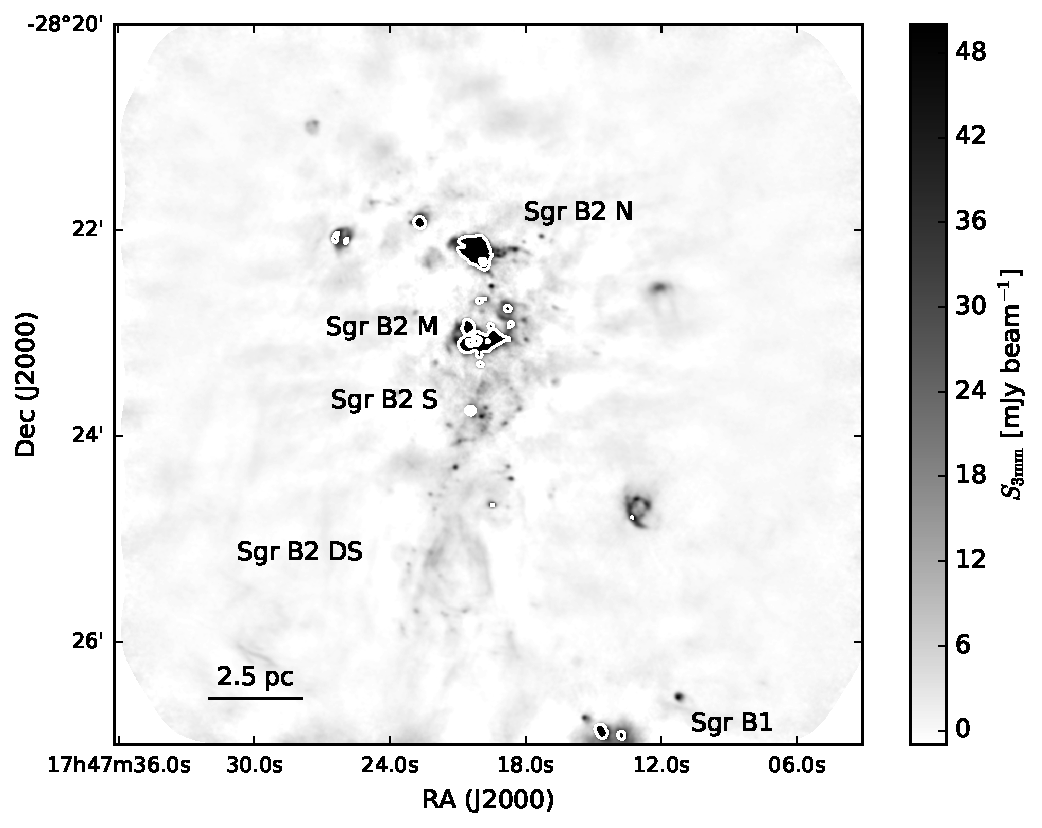
\includegraphics[scale=1,width=\textwidth]{figures/overview_figure_taper_labeled.pdf}
\caption{An overview of the Sgr B2 region, with the most prominent regions labeled.
The image shows the ALMA 3 mm observations imaged with 1.5\arcsec resolution
to emphasize the larger scale emission features.  White contours
are included at [50, 500, 1000, 1500, 2000] mJy/beam to show the flux levels
of the saturated regions.  For a cartoon version of this
figure, see \citet{Schmiedeke2016a} Figure 1.}
\label{fig:overview}
\end{figure*}


The Central Molecular Zone (CMZ) of our Galaxy appears to be overall deficient
in star formation relative to the gas mass it contains
\citep{Beuther2012a,Immer2012a,Longmore2013a,
Kauffmann2017c,Kauffmann2017b,Barnes2017b}.  This deficiency
suggests that star formation laws, i.e., the empirical relations between
the star formation rate and gas surface density, are not universal.  The gas
conditions in the Galactic center are different from those in nearby clouds,
providing a long lever arm in a few
parameters \citep[e.g., pressure, temperature, velocity
dispersion;
][]{Kruijssen2013a,Ginsburg2016a,Immer2016a,Shetty2012a,Henshaw2016a} that
facilitates measurements of the influence of environmental effects on star
formation.

The CMZ dust ridge contains most of the dense molecular material in the
Galactic center \citep{Lis1999a,Bally2010a,Molinari2011a}.  The observed star
formation deficiency comes from comparing the quantity of dense gas to  star
formation tracers such as water masers \citep{Longmore2013a}, infrared source
counts \citep{Yusef-Zadeh2009a}, or integrated infrared luminosity
\citep{Barnes2017b}. 
%The dense gas measurements used in these comparisons
%typically have resolution 10-30\arcsec (0.4-1.2 pc), and the star formation
%measurements have high resolution in the radio ($<1\arcsec$) or rel
%The observations that have demonstrated the star formation deficiency compare
%bulk tracers of star formation to $>0.1$ pc resolution gas observations
%\citep[e.g.,][]{Barnes2017b}.

Recent searches for ongoing star formation using high-resolution millimeter
observations of selected clouds in the CMZ have revealed few star-forming
cores
\citep{Johnston2014a,Rathborne2014a,Rathborne2015a,Kauffmann2017c,Kauffmann2017b}.
As summarized by \citet{Barnes2017b}, most of the dust ridge clouds contain
$<1000$ \msun of stars, or $\sim2\%$ of their mass in stars.
The Sgr B2 N (North), M (Main), and S (South) protoclusters \citep[][Figure
\ref{fig:overview}]{Schmiedeke2016a} are exceptional in that they  are actively
forming star clusters and contain high-mass protostars and many compact \hii
regions \citep[e.g.,][]{Higuchi2015a,Gaume1995a}; despite the active star formation,
the overall cloud appears to be as inefficient as the other dust ridge clouds
\citep{Barnes2017b}. 
Besides Sgr B2, a few of the dust ridge regions are forming stars at a much
lower level, including the 20 \kms and 50 \kms clouds
\citep{Lu2015b,Lu2017a}, Sgr C \citep{Kendrew2013a}, and dust ridge
Clouds C, D, and
E \citep[Walker et al, in prep;][]{Ginsburg2015b,Barnes2017b}.  These regions
contain only a small number of high-mass cores, protostars, and small \hii
regions.

Most observations of the Sgr B2 cloud focus on the ``hot cores'' Sgr B2 N and
M, which are high-mass protoclusters.  The extended cloud has been the subject
of some studies in gas tracers, but it has never been observed at high
($\lesssim10\arcsec$) resolution in the far infrared or millimeter regime.
Radio observations at $\nu<25$ GHz have revealed extended \ammonia and several
masers \citep{Martin-Pintado1999a,McGrath2004a,Caswell2010a}, but these tracers
only detect a subset of star-forming sources.  \citet{Martin-Pintado1999a}
suggested the presence of ongoing star formation in the broader Sgr B2 cloud
based on the detection of three \ammonia (4,4) `hot cores' south of Sgr B2 S.
Despite this suggestion, and the high density of gas throughout the broader Sgr
B2 cloud, an extended star formation event has not been verified.

We report the first observations of extended, ongoing star formation in the Sgr
B2 cloud.  We observed a $\sim15\times15$ pc section of the Sgr B2 cloud and
identified star formation along the entire molecular dust ridge known as Sgr B2
Deep South \citep[DS, also known as the `Southern
Complex'][]{Jones2012a,Schmiedeke2016a}.  These observations allow us to
perform one of the best star-counting based determinations of the star
formation rate within the dense molecular gas of the CMZ.

We adopt a distance to Sgr B2 $D_{\mathrm{Sgr B2}}=\dsgrb$, which is consistent
with Sgr B2 being located in the CMZ dust ridge.  While \citet{Reid2009a}
measure a closer distance of $7.9\pm0.8$ kpc, and \citet{Boehle2016a}
measure a distance to Sgr A$^*$ $7.86\pm0.14$ kpc, we use a value closer to the
IAU-recommended Galactic Center distance of 8.5 kpc, accounting for the
distance difference of $\approx100$ pc measured by
\citet{Reid2009a}\footnote{\citet{Reid2014a} also conclude that the distance to
the Galactic center is 8.34 kpc, suggesting that the direct parallax
measurement to Sgr B2 is underestimated.}.  Choosing the closer distance would
result in masses and luminosities smaller by 12\%, which would not affect any
of the conclusions of this paper.

We describe the ALMA observations and archival single-dish data in Section
\ref{sec:observations}. We focus on the continuum sources selected from the
ALMA data, which we identify in Section \ref{sec:contsources}.  In Section
\ref{sec:analysis}, we perform catalog cross-matching (\S
\ref{sec:crossmatch}), attempt to classify the sources (\S
\ref{sec:classification}), discuss the star formation rate and flux
distribution (\S \ref{sec:distributionsandsfr}), and examine star formation
thresholds.  In the discussion section (\S \ref{sec:discussion}), we discuss
the drivers of star formation in Sgr B2 (\S \ref{sec:whatdrives}) and the
relation between the clusters and the extended star forming population (\S
\ref{sec:clustersandextended}).  We conclude in Section \ref{sec:conclusions}.
Afterward, several appendices describe the single-dish combination (Appendix
\ref{sec:singledishcomb}), self-calibration (Appendix \ref{sec:selfcal}), and
the photometric catalog (Appendix \ref{sec:catalog}).  Two more appendices show
additional figures of \cyanoacetylene (Appendix \ref{sec:hc3nfigures}) and
archival VLA 1.3 cm continuum data (Appendix \ref{sec:onept3cm}).


% pointsource_overlay_deepsouth.py

\begin{figure*}[!htp]
\subfigure[]{ 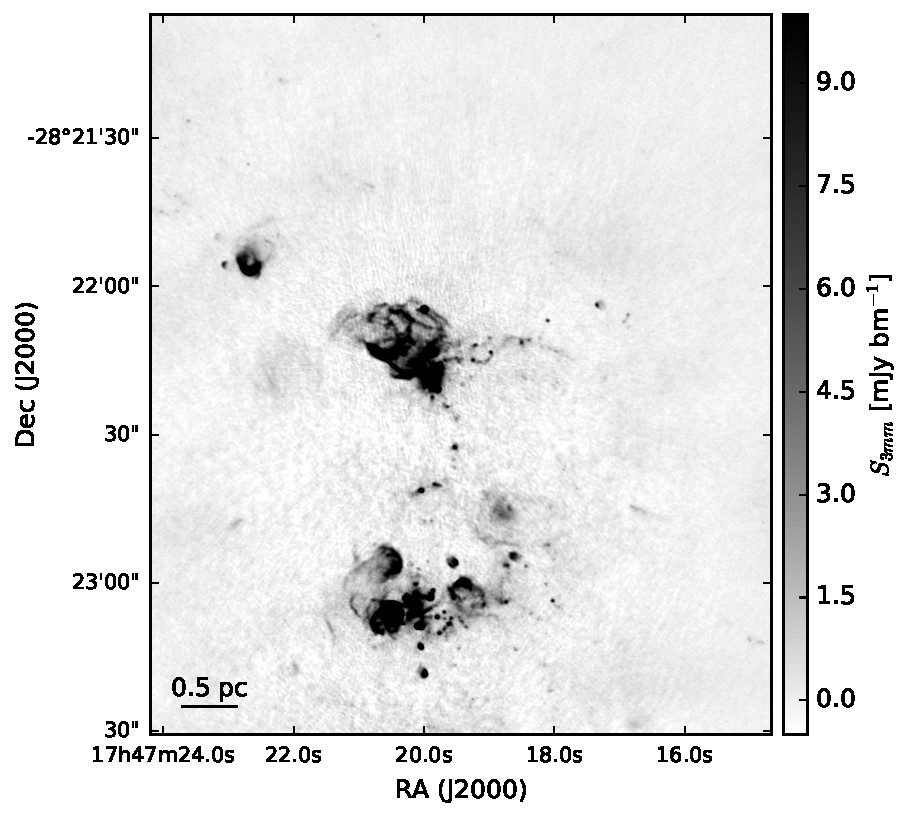
\includegraphics[scale=1,width=0.5\textwidth]{figures/continuum_peak_MandN.pdf} }
\subfigure[]{ 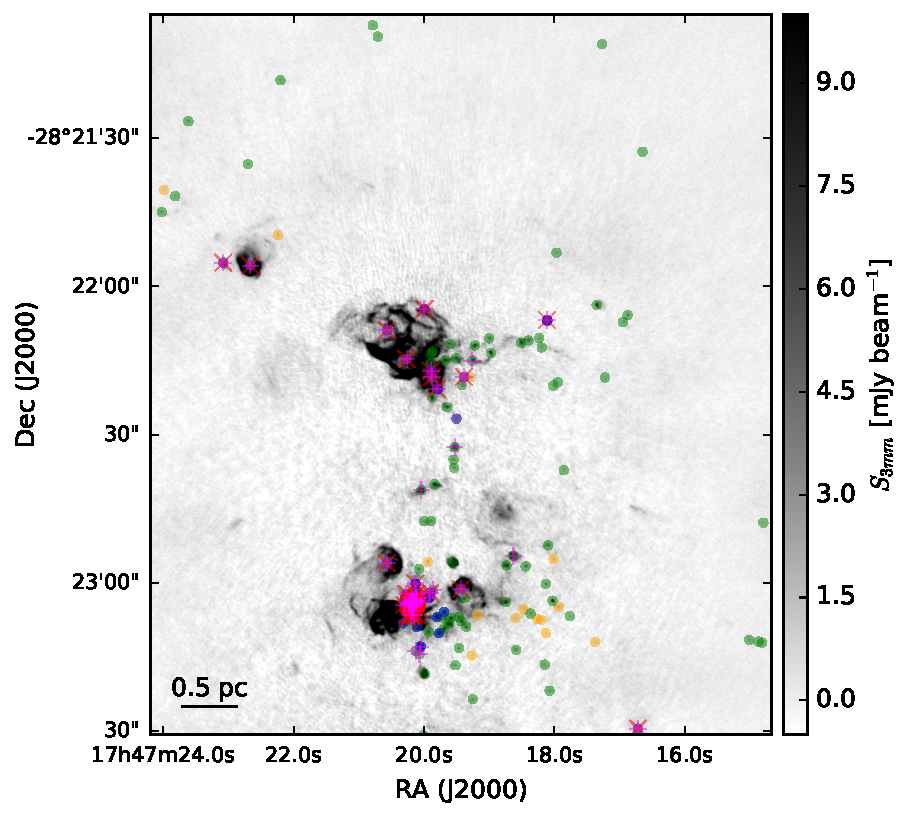
\includegraphics[scale=1,width=0.5\textwidth]{figures/cores_on_continuum_peak_MandN.pdf} }
\caption{Images of the ALMA 3 mm continuum in the Sgr B2 M and N region.  The right
figure additionally includes markers at the position of each identified
continuum pointlike source: red dots are `conservative', high-confidence
sources, orange squares are `optimistic', low-confidence sources, cyan are \hii
regions, magenta +'s are \methanol masers, blue +'s are \water masers, and
green X's are X-ray sources.  The massive
protocluster Sgr B2 M is the collection of \hii regions and compact sources in
the lower half of the image.  The other massive protocluster, Sgr B2 N, is in
the center.
The crowded parts of the images are shown with inset zoom-in panels in
Figure \ref{fig:MandNzooms}.
}
\label{fig:continuumMandN}
\end{figure*}


\section{Observation and Data Reduction}
\label{sec:observations}
\subsection{ALMA data}
Data were acquired as part of ALMA project 2013.1.00269.S (see Table
\ref{tab:observations}).  Observations were taken in ALMA Band 3 with the 12m
Total Power array, the ALMA 7m array, and in two
configurations with the ALMA 12m array.  The setup included the maximum allowed
number of channels, 30720, across 4 spectral windows in a single polarization;
the single-polarization mode was adopted to support moderate spectral
resolution ($\sim0.8$ \kms, 244 kHz channels) across the broad bandwidth.  The
basebands were centered at 89.48, 91.28, 101.37, and 103.23 GHz with bandwidth
1.875 GHz (total 7.5 GHz).  The off position used to calibrate the system
temperature for the Total Power (TP) observations was at J2000 17:52:06.461
-28:30:32.095.


\begin{table*}[htp]
\centering
\caption{Observation Summary}
\begin{tabular}{lllll}
\label{tab:observations}
Date & Array & Observation Duration &  Baseline Length Range  & \# of antennae\\
     &       & seconds              & meters                    & \\
\hline
01-Jul-2014 & 7m & 4045 & 9-49 & 10\\
02-Jul-2014 & 7m & 4043 & 9-49 & 10\\
03-Jul-2014 & 7m & 7345 & 9-48 & 8\\
06-Dec-2014 & 12m & 6849 & 15-349 & 34\\
01-Apr-2015 & 12m & 3464 & 15-328 & 28\\
02-Apr-2015 & 12m & 3517 & 15-328 & 39\\
01-Jul-2015 & 12m & 3517 & 43-1574 & 43\\
02-Jul-2015 & 12m & 10598 & 43-1574 & 42\\

\hline

25-Jan-2015 & TP & 6924  & - & 3\\
01-Apr-2015 & TP & 1986  & - & 2\\
11-Apr-2015 & TP & 6920  & - & 3\\
12-Apr-2015 & TP & 10441 & - & 3\\
25-Apr-2015 & TP & 13928 & - & 3\\
26-Apr-2015 & TP & 22562 & - & 3\\
18-May-2015 & TP & 8342  & - & 3\\
\hline
\end{tabular}
\end{table*}

% analysis/measure_dynamic_range.py
The ALMA QA2 calibrated measurement sets were combined to make a single
high-resolution, high-dynamic range data set.  We imaged the continuum jointly
across all four basebands (without excluding any spectral line regions) using
CASA (version 4.7.2-REL r39762) \texttt{tclean}, and found that the central
regions surrounding Sgr B2 M were severely affected by artifacts that could not
be cleaned out.  We
therefore ran 3 iterations of phase-only self-calibration and two iterations of
amplitude + phase self-calibration, the latter using multi-scale
multi-frequency synthesis with two Taylor terms \citep{Rau2011a}, to yield a substantially
improved image (see Appendix \ref{sec:selfcal}).  The total dynamic range,
measured as the peak brightness in
Sgr B2 to the RMS noise in a signal-free region of the combined 7m+12m image,
is 18000 (noise $\sim0.09$ mJy/beam, 0.05 K), while the dynamic range within one
primary beam ($\sim0.5$\arcmin) of Sgr B2 M is only 5300 (noise $\sim0.3$
mJy/beam, 0.16 K).  Because of the dynamic range limitations and an empirical
determination that clean did not converge if allowed to go too deep, we cleaned
to a threshold of 0.1 mJy/beam over all pixels with $S_\nu > 2.5$ mJy / beam
as determined from a previous iteration of \texttt{tclean}.
The final image used for most of the analysis in this paper was imaged with 
Briggs robust parameter 0.5, achieving a beam size $0.54\arcsec\times0.46\arcsec$.
% We performed this same
% process for both the longest-baseline data only (resolution $\sim0.5\arcsec$,
% largest angular scale theoretically 15\arcsec\ [the shortest baseline] but more
% practically $\sim7$\arcsec\ [the 5th percentile baseline length]) and the
% merged 7m + two 12m configuration data.  The merged data are more useful for
% studying extended structures but have lower dynamic range, while the
% long-baseline-only data are excellent for extracting and analyzing pointlike or
% compact sources.


% pointsource_overlay_inset.py

\begin{figure*}[!htp]
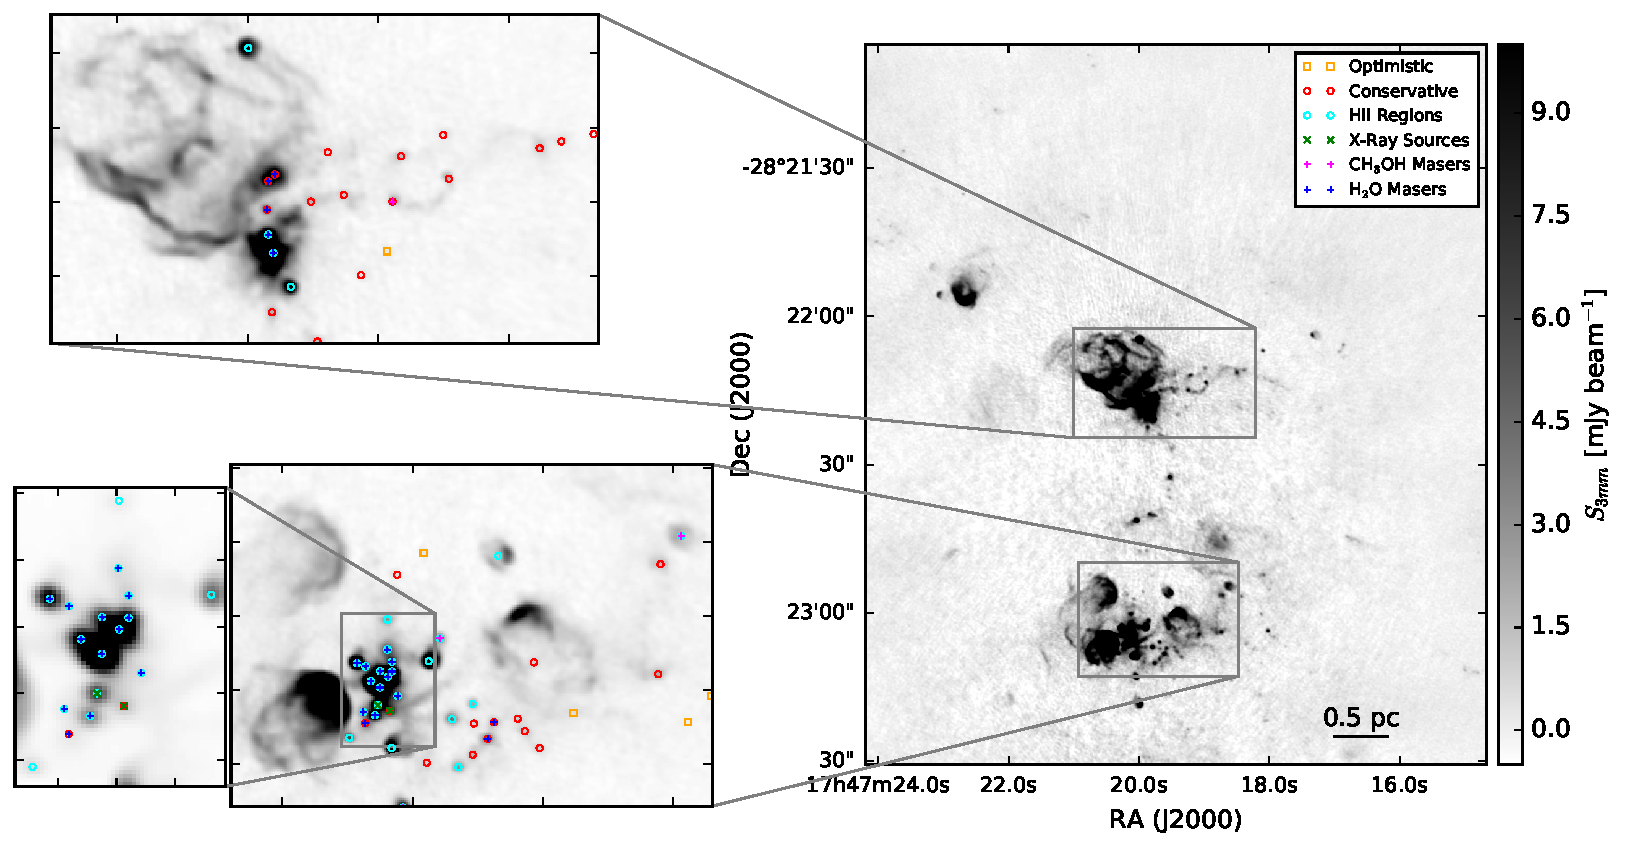
\includegraphics[scale=1,width=\textwidth]{figures/cores_on_continuum_peak_MandN_zoomin_legend.pdf}
\caption{A close-in look at the Sgr B2 M and N region.  Multiple insets show identified
sources in some of the richer sub-regions.  The points are colored as in Figure
\ref{fig:continuumMandN}.  The background image is the ALMA 3 mm continuum.
See also Figure \ref{fig:MandNzoomsVLA}.}
\label{fig:MandNzooms}
\end{figure*}


We also produced full spectral data cubes.  These were lightly
cleaned with a maximum of 2000 iterations of cleaning to a threshold of 100
mJy/beam.  The noise is typically $\approx9$ mJy \perbeam (6 K) per 0.8 \kms
channel in the robust 0.5 cubes.
No self-calibration was applied, both because the dynamic range
limitations were less significant and because the image cubes are
computationally expensive to process.
Before continuum subtraction, dynamic range related artifacts similar to those
in the continuum images were present, but these structures are nearly identical
across
frequencies, and were therefore removable in the image domain.  We use
median-subtracted cubes (i.e., spectral cubes with the median along each spectrum
treated as continuum and subtracted) for our analysis of the lines, noting that
the only location in which an error $>5\%$ on the median-estimated continuum is
expected
is the Sgr B2 North core \citep[][Sanchez-Monge et al. 2017,
submitted]{Sanchez-Monge2017a}.
While many lines were included in the spectral setup, only \cyanoacetylene
J=10-9 is discussed here; of the included lines, it is the brightest and most
widely detected.  This line has a critical density $n_{cr}\equiv A_{ij}/C_{ij}
\approx5\ee{5}$ \percc \citep{Green1978b}, so it would traditionally be
considered a high-density gas tracer.

% pointsource_overlay_deepsouth? (or pointsource_overlay)

\begin{figure*}[!htp]
\subfigure[]{ 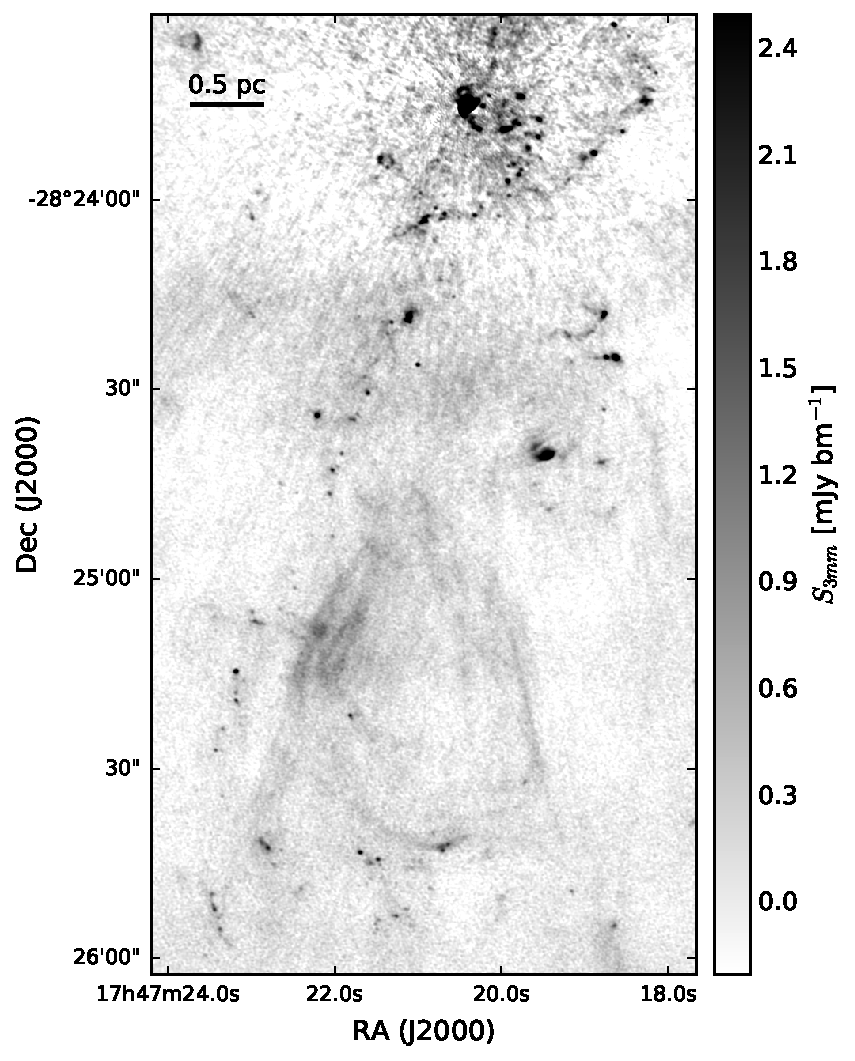
\includegraphics[scale=1,width=0.5\textwidth]{figures/continuum_peak_DeepSouth_saturated.pdf} }
\subfigure[]{ 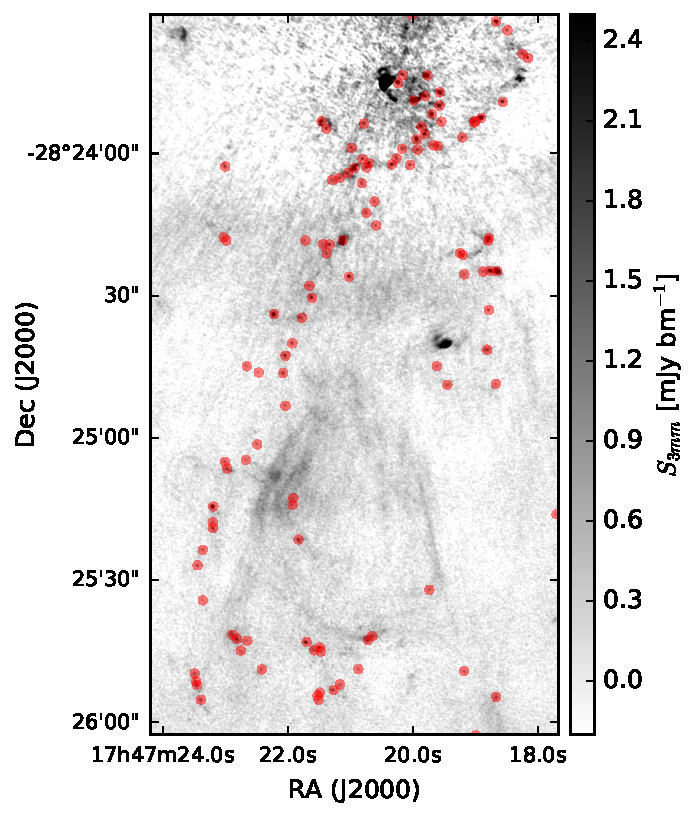
\includegraphics[scale=1,width=0.5\textwidth]{figures/cores_on_continuum_peak_DeepSouth_saturated.pdf} }
\caption{Images of the ALMA 3 mm continuum in the Sgr B2 Deep South (DS) region.  
The right figure additionally
includes markers at the position of each identified continuum pointlike
source: red dots are `conservative', high-confidence sources,
orange squares are `optimistic', low-confidence sources,
cyan are \hii regions, magenta +'s are \methanol masers, blue +'s are \water
masers, and green X's are X-ray sources.
The \hii region Sgr B2 S is the bright source at the top of the image;
imaging artifacts can be seen surrounding it.  The largest angular
scales are noisier than the small scales; the $\sim20\arcsec$-wide east-west
ridge at around -28:24:30 is likely to be an imaging artifact.  By contrast,
the diffuse components in the southern half of the image are likely to be real.
The crowded parts of the images are shown with inset zoom-in panels
in Figure \ref{fig:deepsouthzooms}.
}
\label{fig:continuumDS}
\end{figure*}


The processed data are available from \url{https://doi.org/10.11570/17.0007} in
the form of four $\sim225$ GB data cubes for the full data sets, three
continuum images at different resolutions, and two cubes of \cyanoacetylene at
different resolutions. 

\subsection{Other data - Column Density Maps}
\label{sec:colmaps}
We use archival data to create column density maps at a coarser
resolution than the ALMA data, since the ALMA data are not sensitive
enough to make direct column density measurements.   We use Herschel Hi-Gal
data \citep{Molinari2010a} to perform SED fits to each pixel (Battersby et al,
in prep).  These fits were performed at 25\arcsec resolution, using the 70, 160,
250, and 350 \um data and excluding the 500 \um channel.  The estimated 
uncertainty is $\sim25\%$, with an upper limit on the systematic uncertainty
of a factor of two (Battersby et al, in prep).  To obtain column density maps
with greater resolution, we combine the Herschel data with SHARC 450 \um and
SCUBA 350 \um images.


The CSO SHARC data were reported in \citet{Bally2010a} and have a nominal
resolution of 9\arcsec at 350 \um, however, at this resolution,
the SHARC data display a much higher surface brightness than the Herschel
data on the same angular scale.  An assumed resolution of 11.5\arcsec gives a
better surface brightness match and is consistent with the measured scale of
Sgr B2 N in the image.  This calibration difference is likely to have been a
combination of blurring by pointing errors, surface imperfections, and the
gridding process, which all increase the effective beam size, and flux
calibration errors.  In any case, the Herschel data
provide the most trustworthy absolute calibration scale, since they were taken
from space and calibrated to an absolute scale using Planck data
\citep{Bendo2013a,Bertincourt2016a}.

The JCMT SCUBA 450 \um data were reported in \citet{Pierce-Price2000a} and
\citet{di-Francesco2008a} with a resolution of 8\arcsec.  We found that the
SCUBA data had a flux scale significantly discrepant from the Herschel-SPIRE
500 \um data on 30-90\arcsec scales, even accounting for the central wavelength
difference.  We had to
scale the SCUBA data up by a factor $\approx3$ to make the data agree with
the Herschel-SPIRE images on these scales.  While such a large flux calibration
error seems implausible, it is plausible if the beam size of the ground-based data
is larger than expected.  To assess this possibility, we fit 2D Gaussians to
several sources in the SCUBA CMZ maps, measuring a FWHM toward Sgr B2 N of
approximately 14\arcsec, which means the beam area is $\approx3\times$ larger
in area than the theoretical size.  Among several other sources fit in the
SCUBA map,  the smallest FWHM measured was $\approx10.5$\arcsec.  Between the
larger beam area, flux
calibration errors \citep[quoted at 20\percent in][]{Pierce-Price2000a}, and
the dust emissivity correction (35-50\percent for $\beta=3-4$), this large flux
scaling factor is plausible. This large correction factor is consistent with
the large error beam found by \citet{di-Francesco2008a}, with effective FWHM
$\approx17.3$\arcsec, since they used additional smoothing when creating their
maps.  As with the SHARC data above, we trust the space-based calibration
over the ground-based.


To obtain higher resolution column density maps, we used the combined
Herschel-SPIRE+SHARC and Herschel-SPIRE+SCUBA maps.
%We combined the SHARC and SCUBA data with Herschel SPIRE 350 and 500 \um
%images \citep{Molinari2010a}, respectively.   
We created several column density maps, some assuming arbitrary constant
temperatures equal to the minimum and maximum expected dust temperatures (20
and 50 K), and another using the temperature measured with Herschel
interpolated onto the higher-resolution SCUBA and SHARC grids.  Because of the
interpolation and fixed temperature assumptions, the column maps are not very
accurate and should not be used for systematic statistical analysis of the
column density distribution (i.e., PDF shape analysis) without careful
attention to
the large implied
uncertainties.  However, these higher-resolution data are used in this paper
to provide the best estimates of the local column density around our sample
of compact millimeter continuum sources.
The data combination is discussed in more detail in Appendix
\ref{sec:singledishcomb}.

\section{Analysis}
\label{sec:analysis}
The analysis section includes catalog cross-matching (\S
\ref{sec:crossmatch}), source classification (\S
\ref{sec:classification}), discussion of the star formation rate and flux
distribution (\S \ref{sec:distributionsandsfr}), and examination of star formation
thresholds (\S \ref{sec:thresholds}) and relations (\S \ref{sec:gutermuth}). 

\subsection{Continuum Source Identification}
\label{sec:contsources}
We selected compact continuum  sources by eye,
scanning across images with different weighting schemes (different robust
parameters).  An automated selection is not viable across the majority of the
observed field for several reasons:
\begin{enumerate}
    \item There are many extended \hii regions that dominate the overall map
        emission.  These are clumpy and have local peaks that would dominate
        the identified source population using most source-finding algorithms.
    \item There are substantial imaging artifacts produced by the extremely
        bright emission sources in Sgr B2 M ($S_{3 \textrm{mm,max}} \approx 1.6$ Jy) and
        Sgr B2 N ($S_{3 \textrm{mm,max}} \approx 0.3$ Jy) that make automated source
        identification particularly challenging in the most source-dense
        regions.  These are `sidelobes' from the bright sources that cannot be
        entirely removed.
    \item Resolved-out emission has left multi-scale artifacts throughout the
        images.  While these can be filtered out to a limited degree by
        excluding large angular scales (short baselines), there remain
        small-scale ripples, and the noise increases when baselines are
        excluded.
\end{enumerate}
All of these features are evident in Figures \ref{fig:continuumMandN} and
\ref{fig:continuumDS}. 

Because the noise varies significantly across the map (it is higher near Sgr B2
M), and because there is extended emission, a uniform selection criterion is
not possible.  We therefore include two levels of source identification, `high
confidence' sources, which are selected conservatively in regions of
low-background, and `low-confidence' sources that are somewhat lower
signal-to-noise and are often in regions with higher background (labeled
`conservative' and `optimistic', respectively, in Figure \ref{fig:fluxhist} and
\ref{fig:alphahist}); the difference between the criteria is subjective.  
We measure the local noise for each source by taking the
median absolute deviation in an annulus 0.5 to 1.5\arcsec around the source
center; these noise measurements are reported in Table \ref{tab:photometry}.

Outside of the dense clusters, every locally 5-$\sigma$ peak was visually
inspected.  Peaks that were part of extended structures but not significantly
different from them (e.g., a 5-$\sigma$ peak sitting on a 4-$\sigma$ extended
structure) were excluded.  We excluded sources with extents $r>1\arcsec$
($r>0.04$ pc), i.e., extended \hii regions.

% %TODO: check
% All but 7 sources have signal-to-local-noise ratios $S/N>7$.  These
% sources are all in regions of particularly high background or source
% density and therefore have overestimated local noise.

Our selection criteria result in a reliable but potentially incomplete catalog;
because we did not employ an automated source identification algorithm, we
cannot readily quantify our completeness.  The regions most likely
to be incomplete near our noise threshold are Sgr B2 M and N.  In these
regions, dynamic range limitations increase the background noise and make
fainter sources difficult to detect, as described in Section
\ref{sec:observations}.  Additionally, they both contain extended structures,
including \hii regions and dust filaments, which likely obscure compact
sources.


% The majority of the sources are unresolved.  Some of these sit within regions
% of extended emission.  A small handful were moderately resolved, including some
% of the known \hii regions.

For a subset of the sources, primarily the brightest, we measured the spectral
index $\alpha$ based on CASA \texttt{tclean}'s  2-term Taylor expansion model
of the data (parameters \texttt{deconvolver=`mtmfs'} and \texttt{nterms=2}).
This measurement is over a narrow frequency range ($\approx90-100$ GHz).
\texttt{tclean} produces $\alpha$ and $\sigma(\alpha)$ (error on $\alpha$)
maps, and we used the $\alpha$ value at the position of peak intensity for each
source.  We include in the analysis only those sources with $|\alpha| > 5
\sigma(\alpha)$ or $\sigma(\alpha) < 0.1$; the latter include sources with
$\alpha\sim0$ measured at relatively high precision.  \nalphas sources met these
criteria. Several of the brightest sources did not have significant
measurements of $\alpha$ because they are in the immediate neighborhood of Sgr
B2 M or N and therefore have significantly higher background and noise,
preventing a clear measurement.  To check the calibration of the spectral index
measurement, we imaged one of our calibrators, J1752-2956, and obtained a
spectral index $\alpha=-0.62\pm0.14$, consistent with the expected
$\alpha\approx-0.7$ for an optically thin synchrotron source
\citep[e.g.,][]{Condon2007a}.  We also note that the \emph{relative} spectral
index measurements in our catalog should be accurate, since all sources come
from the same map with identical calibration.


\begin{figure*}[!htp]
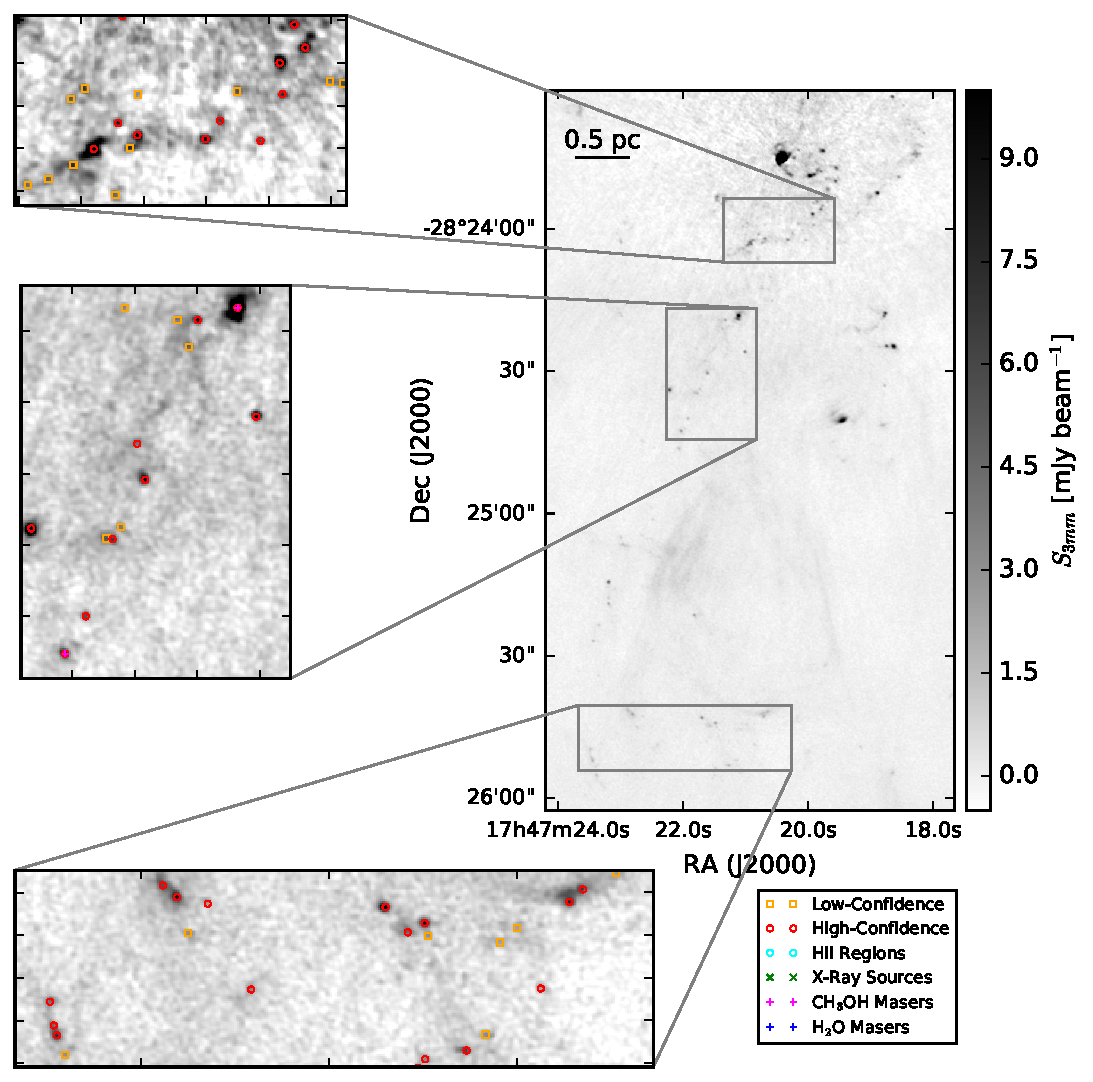
\includegraphics[scale=1,width=\textwidth]{figures/cores_on_continuum_peak_DeepSouth_zoomin_legend.pdf}
\caption{A close-in look at the Sgr B2 DS region.  Multiple insets show identified sources
in some of the richer sub-regions.  The points are colored as in Figure
\ref{fig:continuumMandN}.  The background image is the ALMA 3 mm continuum.}
\label{fig:deepsouthzooms}
\end{figure*}


We detected \ncores compact continuum sources, and they are listed
in Table \ref{tab:photometry}.  Their flux distribution is
shown in Figure \ref{fig:fluxhist}.  The distribution of their measured
spectral indices $\alpha$ is shown in Figure \ref{fig:alphahist}.
Generally, spectral indices $\alpha<0$ indicate nonthermal (e.g., synchrotron)
emission, $-0.1<\alpha<2$ may correspond to free-free sources of various
optical depths, $\alpha=2$ for any optically thick thermal source,
and $\alpha>2$ usually indicates optically thin dust emission.  These indices
will be discussed further in the next Section.

\subsection{Catalog Cross-Matching}
\label{sec:crossmatch}
We cross-matched our source catalog with catalogs of \ammonia sources, \hii
regions, X-ray sources, Spitzer sources, and methanol and water masers.
Associations with these types of sources can be used to classify the sources.

We classified sources as \hii regions if there is a corresponding 0.7 or 1.3 cm
source from one of the previous VLA surveys
\citep{Gaume1995a,Mehringer1995b,De-Pree1996a,De-Pree2015a} within one ALMA
beam (0.5\arcsec).  \nhii of our sources are classified as \hii regions; these
all have $S_{3 \textrm{mm}} > 9$ mJy.  The
majority of these are unresolved, but we have included \hii regions with radii
up to $\approx1\arcsec$ in our catalog.  Optically thick \hii regions (like any
blackbody) have a spectral index $\alpha=2$.  Optically thin \hii regions have
a nearly flat spectral index, $\alpha=-0.1$ \citep{Condon2007a}.   The observed
sources with \hii region counterparts have spectral indices consistent with the
theoretical expectation for optically thin \hii regions in Figure
\ref{fig:alphahist}.  The existing VLA data do not cover the entire area of our
observations, so we only have a lower limit on the number of \hii regions in
our sample; the sources in Sgr B2 DS have not yet been observed in the radio at
high resolution.  Sources matched with \hii regions evidently contain high-mass
(most likely $M\gtrsim20$ \msun, see Section \ref{sec:theyarehiiregions} below)
young stars.
%Several sources (\nhii) in our catalog match known \hii regions from
%\citet{Gaume1995a} to within 0.5\arcsec, most of which are associated with the
%brightest sources in our sample; these all have $S_{3 \textrm{mm}} > 9$ mJy.
%The \citet{Gaume1995a} catalog does not cover the full observed area, so the
%\hii region source association is incomplete.  These sources evidently contain
%high-mass young stars, but they are not `protostars'.


\citet{Martin-Pintado1999a} observed part of Sgr B2 DS and M in \ammonia with
the VLA.  They identified three ``hot cores'' based on \ammonia (4,4) detections.
Only their first source HC1 has an associated 3 mm continuum source, suggesting
that HC2 and HC3 are not genuine hot cores but are some other variant of
locally heated (perhaps shock-heated) gas.  However, the
association between HC1 and our source 43 suggests that it is a young stellar
object with a massive envelope.  Of the 6 \ammonia (3,3) maser sources identified
by \citet{Martin-Pintado1999a}, three are in regions with high 3 mm source
density but lack a clear one-to-one source association, one is coincident with
an \hii region not in our catalog, and two have no obvious associations; the
\ammonia (3,3) masers therefore do not appear to be unambiguous tracers of star
formation in this environment, consistent with the conclusions of
\citet{Mills2015a}.  


Class II methanol masers are exclusively associated with sites of high-mass
star formation.  The \citet{Caswell2010a} Methanol Multibeam (MMB) Survey
identified 11 sources in our observed field of view (their survey covers our
entire observed area), of which \nmasermatch have a clear match to within
1\arcsec of a source in our catalog (the MMB catalog sources have a positional
accuracy of $\approx0.4\arcsec$, but masers may have an extent up to 1\arcsec).
These sources are clearly identified as high-mass protostars.
The single maser that does not have an associated millimeter source is 5\arcsec
west of Sgr B2 S and resides near some very faint and diffuse 3 mm
emission; it is unclear why the 3 mm is so weak here, but it hints that there
are massive young stellar objects (MYSOs) with 3 mm emission below our
detection limit.


Water masers are generally associated with forming young stars.  We
also matched our catalog with the \citet{McGrath2004a} water maser catalog,
finding that 23 of our sources have a water maser within 1\arcsec.
Again, these sources are likely to contain protostars, but not necessarily
MYSOs based on their \water maser detections alone.

Some young stars exhibit X-ray emission, including some MYSOs
\citep[e.g.,][]{Townsley2014a}, so we searched for X-ray emission from our
sources.  \nxraymatch of the sources have X-ray counterparts in the
\citet{Muno2009a} Chandra point source catalog within 1\arcsec.  The
\citet{Muno2009a} catalog covers our entire observed area.  The X-ray
associated sources most likely either contain protostars or young stars.

We searched the \citet{Yusef-Zadeh2009a} catalogs of 4.5 \um excess sources and
YSO candidates and found only one source association, though there are 5 and
14, respectively, of these sources in our field of view.  Two of the 4.5 \um
excess sources and one of the YSO candidates are associated with extended \hii
regions (which we do not catalog); the single association is of a 4.5 \um source with the central region
of Sgr B2 M. By-eye comparison of the Spitzer maps and the ALMA images suggests
that the lack of associations is at least in part because of the high
extinction in the regions containing the 3 mm cores; there are overall fewer
Spitzer sources in these parts of the maps.

Finally, we searched the \citet{Mehringer1997a} sample of 44 GHz Class I \methanol
maser sources for associations, finding no matches with any
of our sources.  This methanol maser line apparently does not trace star
formation.


\subsection{Source Classification}
\label{sec:classification}
For the majority of the detected sources, we have only a continuum detection at
3 mm.    In this section, we employ a variety of arguments to classify the
sample of new sources.  Most of our sources have no match in other catalogs
(see Section \ref{sec:crossmatch}), so we discuss what types of objects they
could be given their 3 mm continuum detections.  Plausible emission mechanisms
include free-free and thermal dust emission, so we explore whether the sources
could be different classes of free-free sources: externally ionized
globules (\S \ref{sec:alt1}), \hii regions from an extended population of
OB stars (\S \ref{sec:alt2}), or \hii regions around young massive stars (\S
\ref{sec:theyarehiiregions}).  We conclude that they are
primarily dusty sources (\S \ref{sec:theyareprotostars}).

We visually inspected the spectra extracted from the full line cubes, and no
lines are detected peaking toward the majority of the sources (most sources
have emission in some lines (e.g., \cyanoacetylene), but this emission is
clearly extended and not associated with the compact source).  Given the
relatively poor line sensitivity (RMS $\approx 6$ K), the dearth of detections
is not very surprising.  We therefore cannot use spectral lines to classify
most sources.


% core_flux_distributions
%\FigureOneCol{figures/core_peak_fluxdensity_powerlawfit.png}

\begin{figure}[!htp]
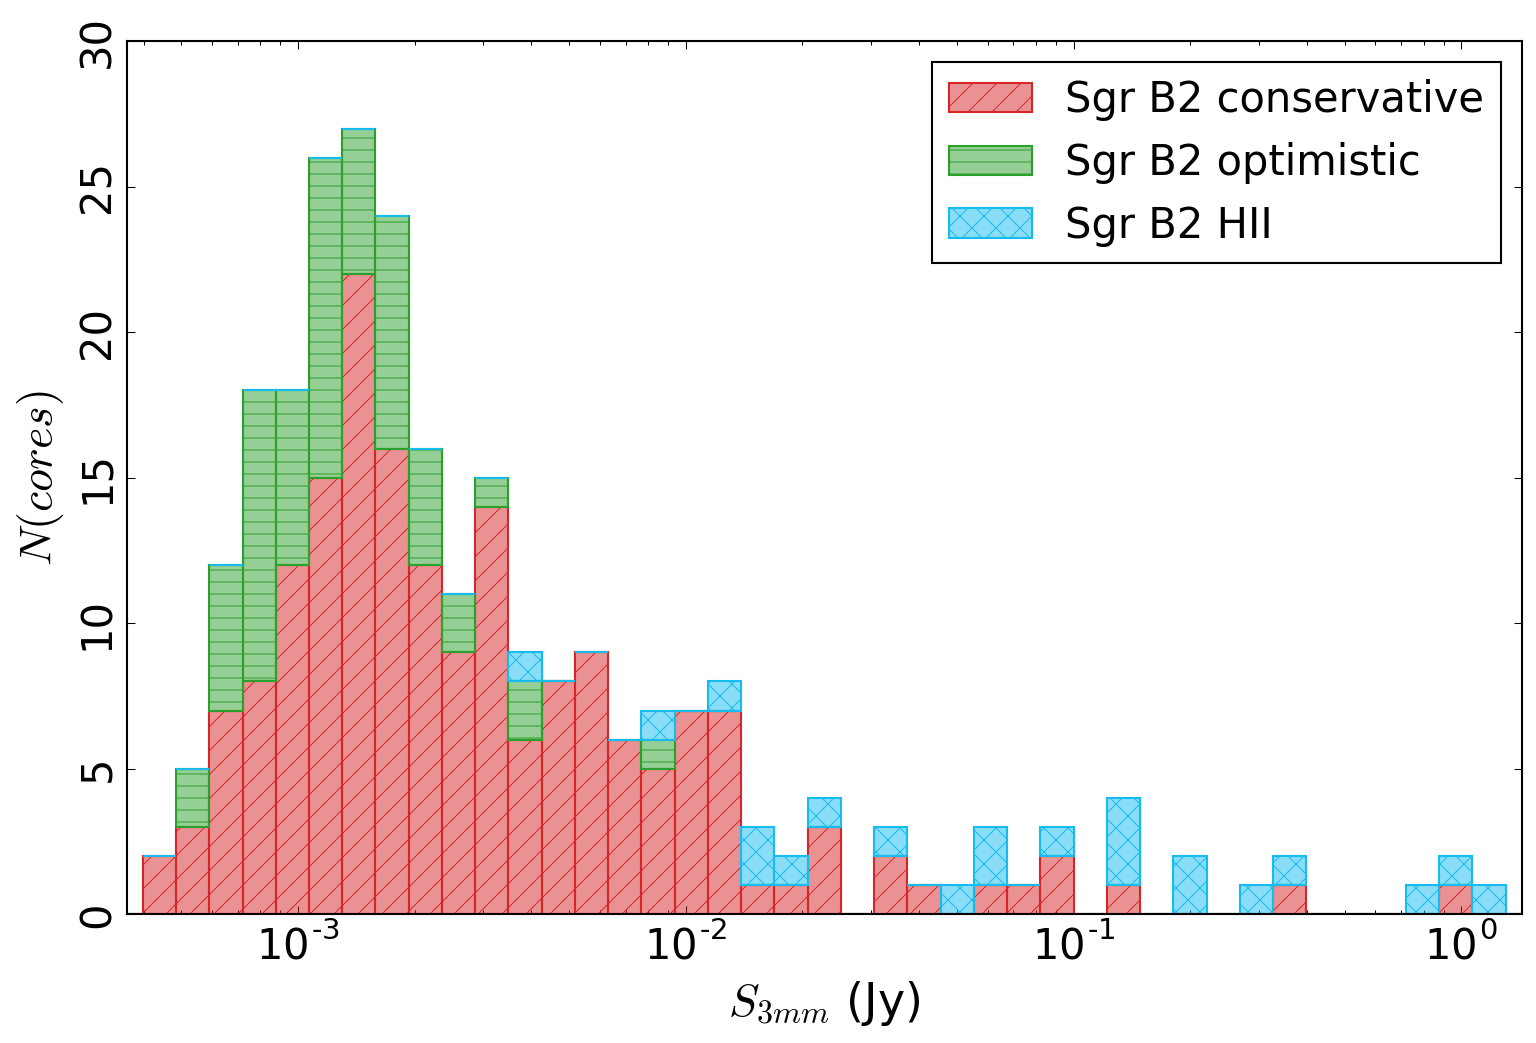
\includegraphics[scale=1,width=0.5\textwidth]{figures/core_peak_fluxdensity_coloredbyclass.png}
\caption{A histogram of the flux density (the peak intensity converted to flux density
assuming the source is unresolved) of the observed sources. 
The histograms are stacked such that there are a total of 27 sources in the
highest bin.
}
\label{fig:fluxhist}
\end{figure}


To aid in our classification, we note some properties of dust at 3 mm.  The
simplest assumption is that all sources we have detected that were not detected
at longer wavelengths are pure dust emission sources at a constant temperature.
At \dsgrb, a 1 mJy source corresponds to an optically thin gas mass\footnote{We
assume a gas-to-dust ratio of 100 throughout this work.} of
$M(40\mathrm{K})=18$ \msun or $M(20\mathrm{K})=38$ \msun assuming a dust
opacity index $\beta=1.75$ ($\alpha=3.75$ on the Rayleigh-Jeans tail) to
extrapolate the \citet[][MRN with thin ice mantles anchored at
1mm]{Ossenkopf1994a} opacity to $\kappa_{3.1 \mathrm{mm}}=0.0018$ cm$^2$
g$^{-1}$ (per gram of gas).  Our dust-only (i.e., excluding free-free emission)
5-$\sigma$ sensitivity limit at 20 K therefore ranges from $M>19$ \msun (0.5
mJy) to $M>94$ \msun (2.5 mJy) across the map.  If we were to assume that these
are all cold, dusty sources, as is typically (and reasonably) assumed for local
clouds, they would be extremely massive and dense, with the lowest measurable
density being $n(20\mathrm{K}) > 1\ee{8}$ \percc (corresponding to 19 \msun in
an $r=0.2$\arcsec$=1700$ AU radius sphere, i.e., a sphere with radius equal
to the beam $1-\sigma$ size).  Such extreme objects are possible,
but since we have detected $>100$ of these sources, we evaluate other
possibilities.

We start with a few alternatives we are able to rule out: externally
ionized gas globules, internally ionized \hii regions from an older
generation of `interloper' stars, and internally ionized \hii regions
from a newly-formed generation of massive stars.  We then discuss
why these sources are most likely embedded protostars.


\subsubsection{Alternative 1: The sources are externally ionized gas blobs}
\label{sec:alt1}
One possibility is that these sources are not dust-dominated, nor pre- or
protostellar, but are instead externally ionized, mostly neutral gas clumps
embedded within diffuse \hii regions.  They would then be analogous to the
heads of cometary clouds, externally ionized globules
\citep[``EGGs"][]{Sahai2012a}, or proplyds (externally ionized protoplanetary
disks), and their observed emission would give little clue to their nature because
the light source is extrinsic.

The majority of the detected sources have size $<4000$ AU, i.e., they are
unresolved.  By contrast, the free-floating EGGs (`frEGGs') so far observed have sizes
10,000-20,000 AU \citep{Sahai2012a,Sahai2012b}, so they would be resolved in
our observations.  Toward the brightest frEGG in Cygnus X, \citet{Sahai2012b}
measured a peak intensity $S_{8.5 GHz} \approx 1.5$ mJy/beam in a
$\approx3\arcsec$ beam.  Cygnus X is $6\times$ closer that the Galactic center,
so their beam size is the same physical scale as ours.  If the free-free
emission is thin ($\alpha=-0.1$), the brightness in our data would be $S_{95 GHz} =
(95/8.5)^{-0.1} S_{8.5 GHz} = 0.79 S_{8.5 GHz} \approx 1.2$ mJy/beam.  These
frEGGs would be detectable in our data.  Comparison to radio observations
at a similar resolution will be needed to rule out the externally ionized
globule hypothesis for the resolved regions within our sample, but the unresolved
sources are unlikely to be frEGGs.

% core_table_plots

\begin{figure}[!htp]
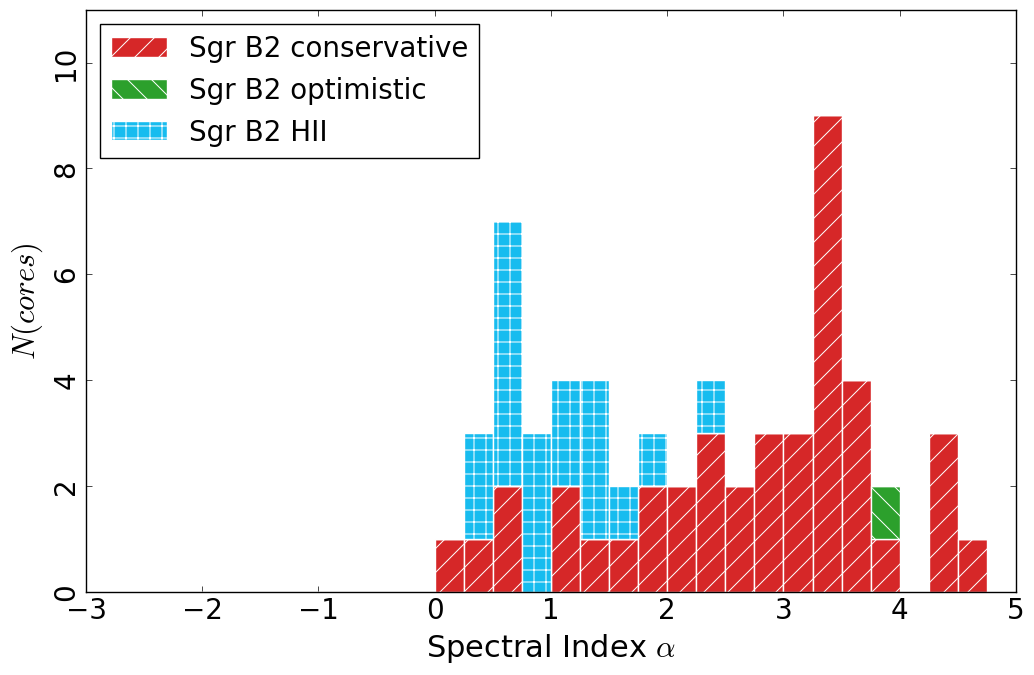
\includegraphics[scale=1,width=0.5\textwidth]{figures/core_alpha_coloredbyclass.png}
\caption{A histogram of the spectral index $\alpha$ for those sources with a statistically
significant measurement.  The \hii regions cluster around $\alpha=0$, as expected
for optically thin free-free emission, while the unclassified sources cluster
around $\alpha=3.5$, which is  consistent with dust emission.
}
\label{fig:alphahist}
\end{figure}


If the detected sources were either EGGs or cometary clouds, we would expect
them to be located within diffuse \hii regions, since that is where all other
sources of this type are seen, and since an external ionizing agent is needed
to illuminate them.  Many of the sources are near \hii regions, as seen in
Figure \ref{fig:coreson20cmandhc3n}a, but not within them.  The sources are
nearly all associated with a ridge of molecular (\cyanoacetylene) emission
(Figure
\ref{fig:coreson20cmandhc3n}b).  If they are deeply embedded within the
molecular material, they cannot be externally ionized.  
%The current data do not provide enough information on the geometry of the
%clouds to rule out the possibility that the point sources are just illuminated
%cloud edges, but 
The fact that the ionized gas is brightest nearby, rather than directly on top
of, the \cyanoacetylene suggests that the \cyanoacetylene traces a full
molecular cloud rather than a thin PDR-like layer, which would be required if
these sources are cometary clouds.  The association with dense molecular gas
implies that the sources are not externally ionized objects.

A final point against the externally ionized hypothesis is the observed
spectral indices shown in Figure \ref{fig:alphahist}.  We measured spectral
indices for \nalphas sources, of which \ngttwo have $\alpha>2$.  These \ngttwo
sources are inconsistent with free-free emission and are at least reasonably
consistent with dust emission.
%Of the 20 that are consistent with free-free emission, 11
%are known \hii regions, hinting that our sample is dominated by dusty objects,
%not externally ionized objects.

%This
%scale is consistent with that of frEGGs seen in Carina \citep[e.g.,][]{Sahai2012a}.
%The flux density of our sources is 1-2 orders of magnitude below what we would
%predict from the dust observed in the \citet{Sahai2012a} object, though the
%free-free... \todo{Look up observed free-free emission from proplyds and frEGGs.
%Could we have frEGGs?}

% The `tadpole' \citep{Sahai2012b} has $S_{22 \mathrm{GHz}} = 30$ mJy at d=1.4 kpc, resolved
% to $\sim10\times10$ arcsec.  In the CMZ... this would be visible.  Maybe compare to Zadeh's
% recent obs of "proplyds"?

% The key requirement, if these are all indeed externally ionized molecular
% blobs, is that of a strong ionizing radiation field.  Indeed, L-band
% observations \citep{Yusef-Zadeh2004a} show that many of these sources are
% located along the outer edges of a large-scale \hii region (Figure
% \ref{fig:coreson20cm}).
% 
% % However, their location poses a problem for the
% % frEGG/proplyd hypothesis: % this next sentence doesn't really make sense...
% %these sources are observed \emph{within} \hii
% %regions, not along their outskirts. 
% However, when analogous structures are present
% along the outskirts of clouds, they are usually accompanied by a larger
% contiguous cloud edge, which results in a continuous sharp-edged bright feature
% corresponding to a PDR.  Such edges are seen in the Orion Bar and M16's
% ``Pillars of Creation''.   We do not observe any such features here.
% 
% We know from our molecular line observations in HC$_3$N that most of the
% continuum sources lay along a molecular ridge (TODO: FIGURE), so it appears
% most of these sources are embedded in molecular material.

% Nice idea, but h41a is just too weak
% TODO: H41a TE peak map.  Show locations relative to confirmed HII regions

%% pointsource_overlay
%\FigureOneCol{figures/cores_on_20cm_continuum.png}
%{The location of the detected continuum sources (red points) overlaid on a 20
%cm continuum VLA map highlighting the diffuse free-free (or possibly
%synchrotron) emission in the region \citep{Yusef-Zadeh2004a}.}
%{fig:coreson20cm}{1}{0.5\textwidth}
%
%% pointsource_overlay
%\FigureOneCol{figures/cores_on_HC3N_peak.png}
%{The location of the detected continuum sources (red points) overlaid on a map
%of the HC$_3$N peak intensity.  HC$_3$N traces moderate-density molecular gas.}
%{fig:coresonhc3n}{1}{0.5\textwidth}

% pointsource_overlay.py

\begin{figure*}[!htp]
\subfigure[]{ 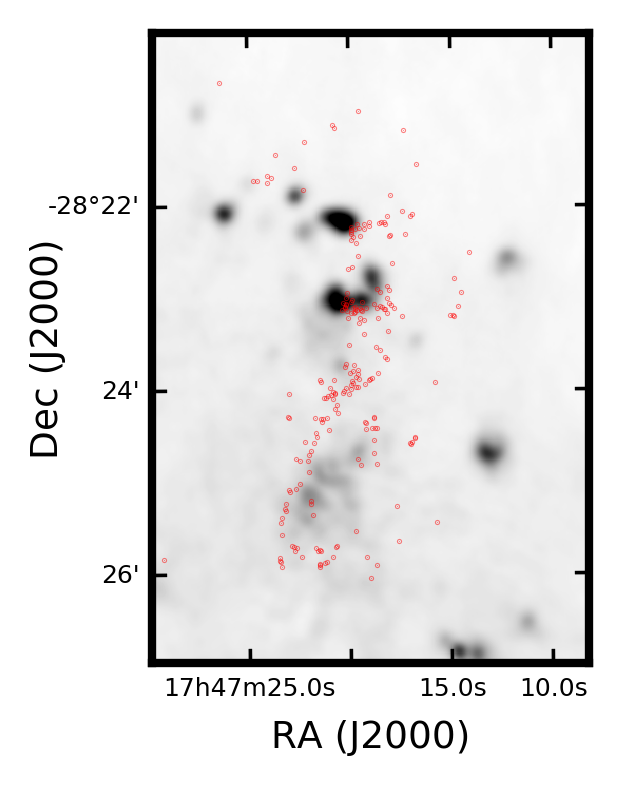
\includegraphics[scale=1,width=0.5\textwidth]{figures/cores_on_20cm_continuum.png} }
\subfigure[]{ 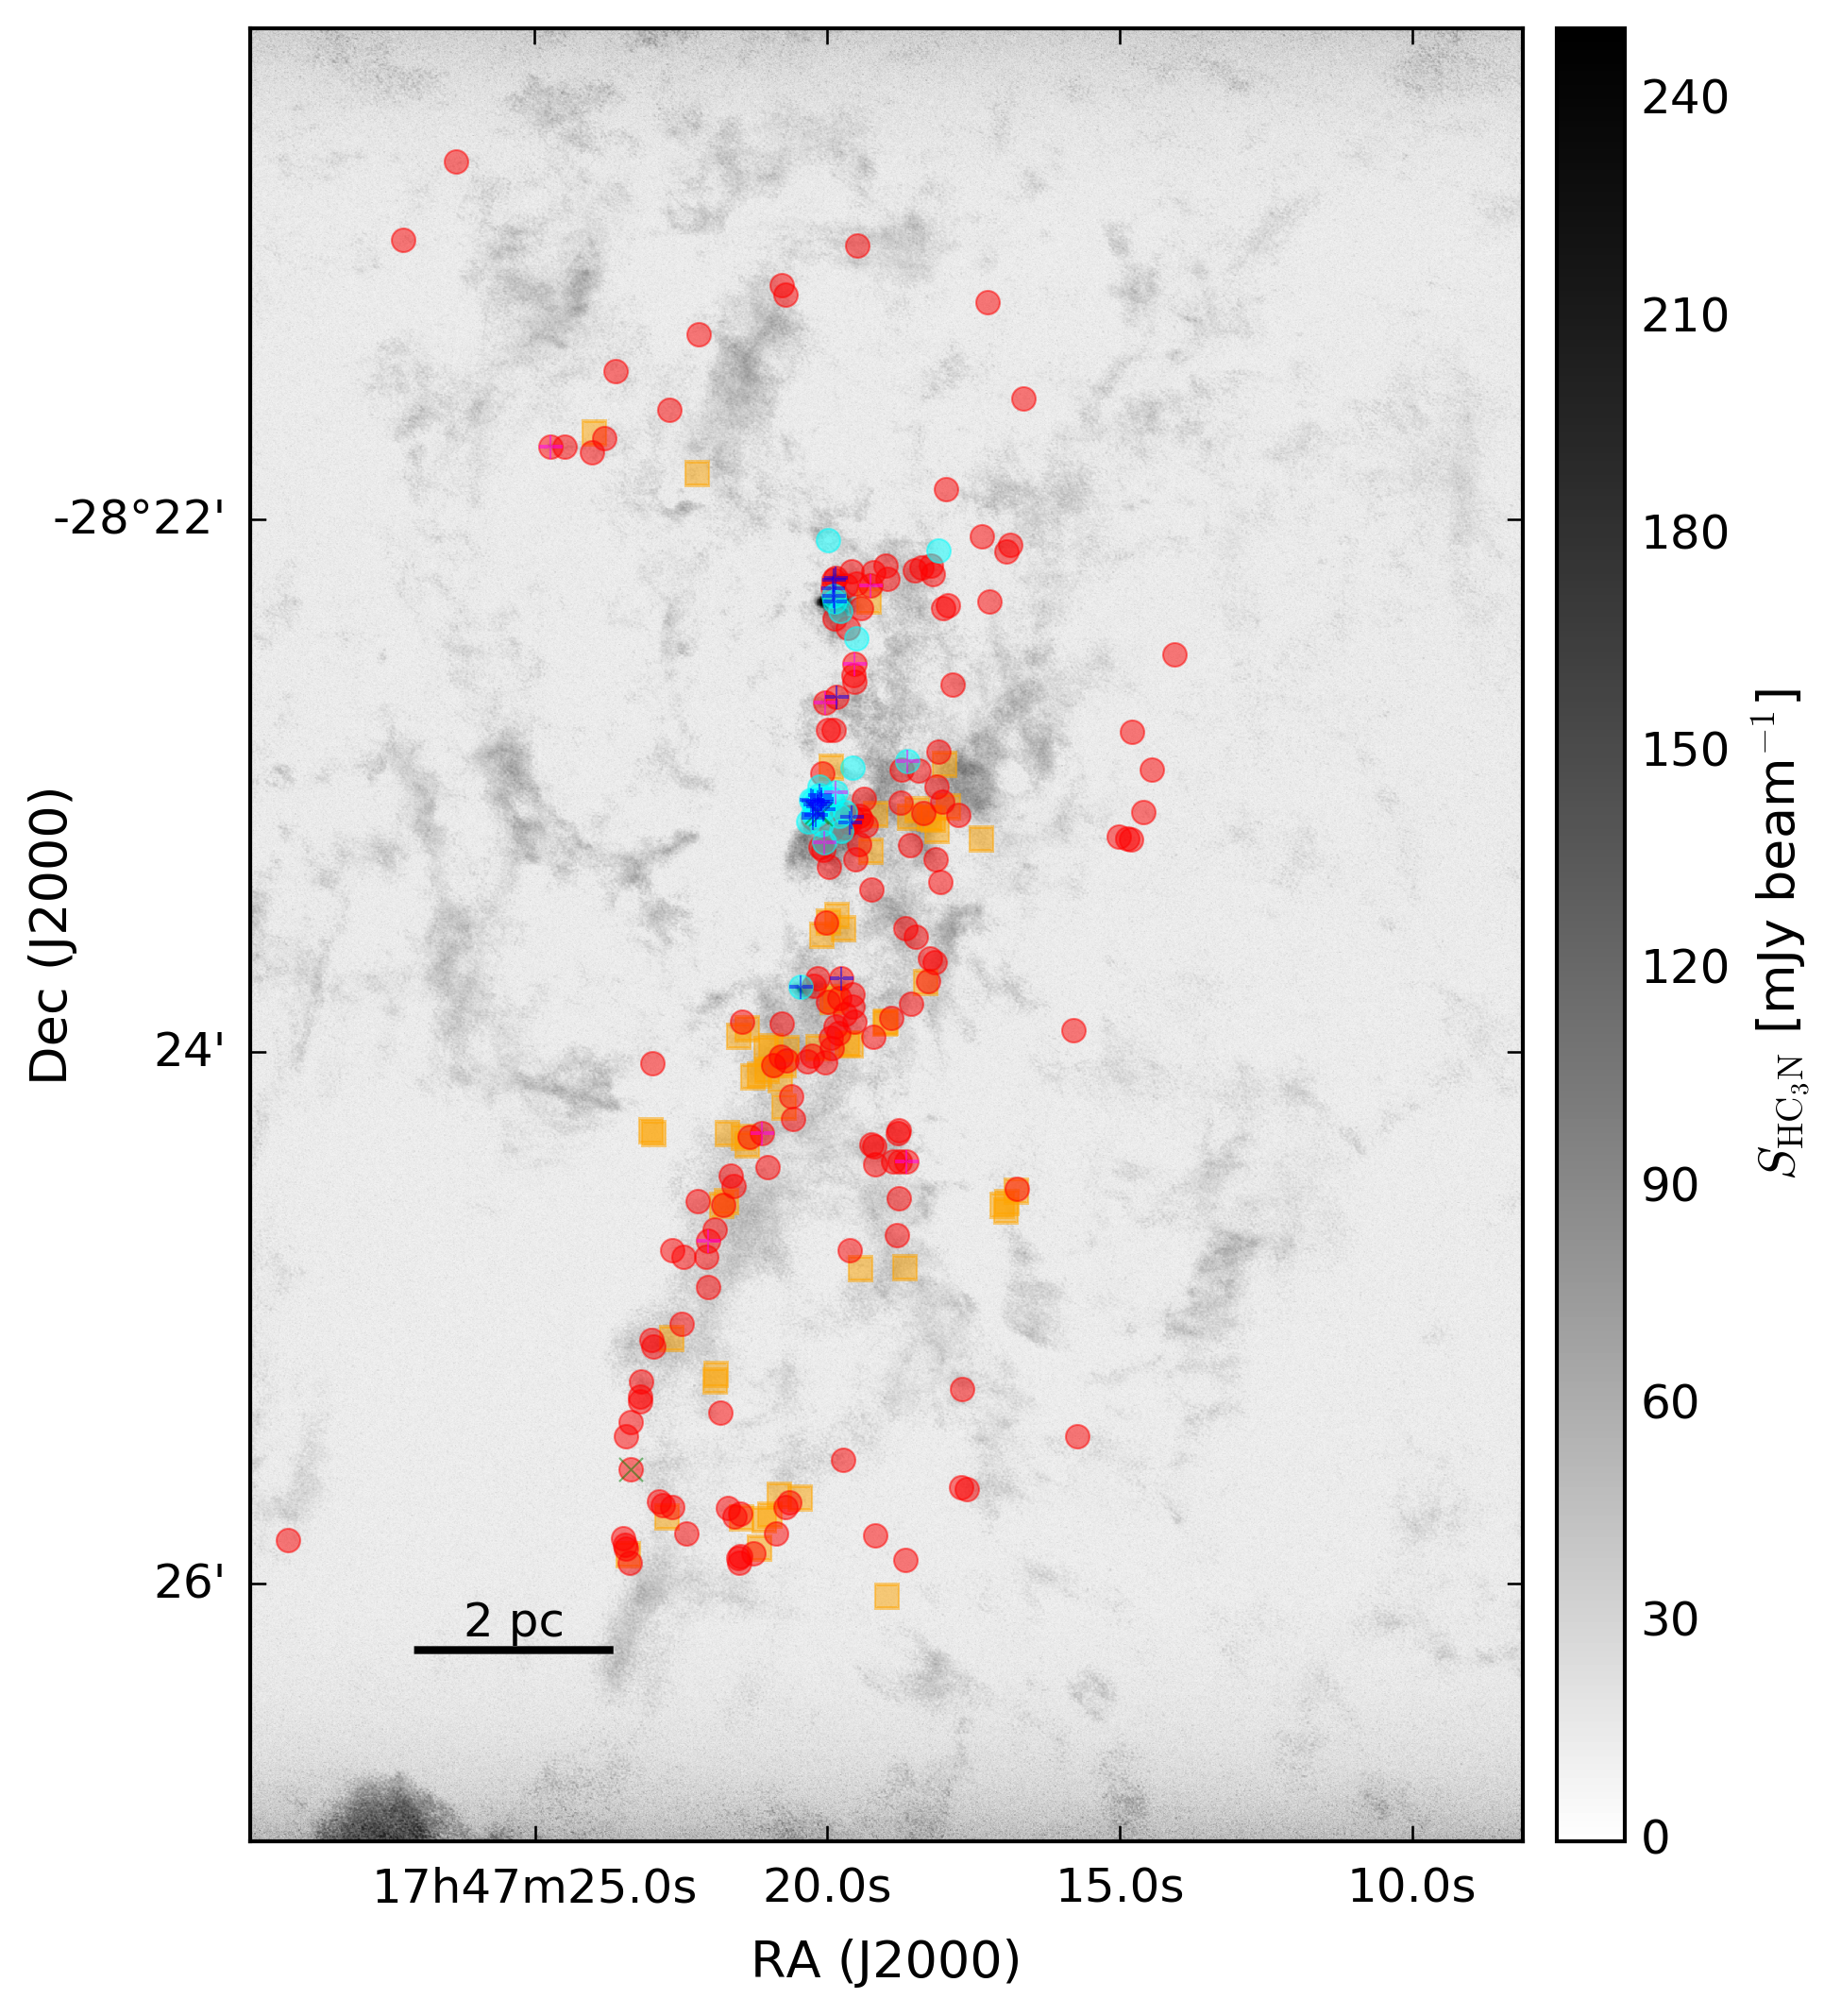
\includegraphics[scale=1,width=0.5\textwidth]{figures/cores_on_HC3N_peak.png} }
\caption{(left) The location of the detected continuum sources (red points) overlaid on a 20
cm continuum VLA map highlighting the diffuse free-free (or possibly
synchrotron) emission in the region \citep{Yusef-Zadeh2004a}.
(right) Continuum sources overlaid on a map
of the \cyanoacetylene J=10-9 peak intensity over the range [-200, 200] \kms.
  In both figures, red
dots are `conservative',
high-confidence sources, orange squares are `optimistic', low-confidence sources,
cyan are \hii regions, magenta +'s are \methanol masers, blue +'s are \water
masers, and green X's are X-ray sources.
}
\label{fig:coreson20cmandhc3n}
\end{figure*}


\subsubsection{Alternative 2: The sources are \hii regions produced by
interloper ionizing stars}
\label{sec:alt2}
If there is a large population of older (age 1-30 Myr) massive stars, they
could ignite compact \hii regions when they fly through molecular material.  In
other words, each OB star that encounters dense enough gas would create a
compact \hii region that would not have time to expand due to the star's rapid
motion.  Such sources would be bow-shaped when viewed at higher resolution.
See \ref{sec:theyarehiiregions} for calculations of stationary \hii region
properties.

The main problem with this scenario is the spatial distribution of
the observed sources.  While most of the continuum sources are associated with
dense gas and dust ridges, not all of the high-column molecular gas regions
have such sources in them (i.e., 
Figure \ref{fig:coreson20cmandhc3n}b, where molecular material is seen with no
associated millimeter sources outside of the north/south \cyanoacetylene
ridge).  If there is a free-floating population of OB
stars responsible for the 3 mm compact source population, and if we assume the
spatial distribution of the stars is uniform, the distribution of \hii regions
surrounding them should match that of the gas. 
  Also, there is no such population of sources
seen \emph{outside} of the dense gas in the infrared,
%\citep[TODO: Who has done
%infrared studies of Sgr B2?  You can infer what I have stated `by inspection'
%of 2MASS, but it would be more straightforward to quote someone else][]{},
which again we should expect if there is a uniformly distributed massive stellar
population.  Finally, the spectral indices discussed above (Figure
\ref{fig:alphahist}) suggest the previously-unidentified sources are dust
emission sources, not
free-free sources.



\subsubsection{Alternative 3: The sources are \hii regions produced by
recently-formed OB stars}
\label{sec:theyarehiiregions}

We know from previous observations
\citep[e.g.,][]{Mehringer1995b,De-Pree1996a,De-Pree2015a} that there is a
substantial population of \hii regions in the Sgr B2 clusters.  The \nhii
sources associated with these previously-identified \hii regions are among the
brightest in our catalog.  We address here whether the remaining  sources,
which are mostly fainter, could also be \hii regions.

For an unresolved spherically symmetric \hii region ($R=4000$ AU), the expected
flux density is $S_{95 \mathrm{GHz}} = 4.7$ mJy for a $Q_{lyc}=10^{47}$ \pers
source (assuming $T_e=7000$ K), and that value scales linearly with $Q_{lyc}$
as long as the source is optically thin.   We rearrange \citet{Condon2007a}
equations 4.60 and 4.61 to get the expected flux density as a function of
temperature, emission measure, and frequency:
\begin{eqnarray}
S_{\nu}(Q_{lyc})  &=& 4.67 \left[1-\exp\left(c_* T_* \nu_* EM_* \right) \right] \nonumber \\
\nu_* &=& \left(\frac{\nu}{\mathrm{GHz}}\right)^{-2.1} \nonumber \\
T_* &=& \left(\frac{T_e}{10^4 \mathrm{K}}\right)^{-1.35} \nonumber \\
c_* &=& -3.28\times10^{-7} \nonumber \\
EM_* &=& \frac{3 Q_{lyc}}{4 \pi R^2 \alpha_B} \nonumber \\
\end{eqnarray}
where the case-B recombination coefficient $\alpha_B=2\ee{-13}$ cm$^3$
s$^{-1}$, $Q_{lyc}$ is the count rate of ionizing photons in $s^{-1}$, and $R$
is the \hii region radius.  The constant $c_*$ was computed by
\citet{Mezger1967a} as an approximation to the optical depth prefactor in the
full radiative transfer equation and is never incorrect by more than
$\approx25\%$.

An extremely compact \hii region,
e.g., one with $R<100$ AU and corresponding density $n>10^6$ \percc, would be
optically thick and therefore fainter, $S_{95 \mathrm{GHz}}(R=100 \mathrm{AU},
Q_{lyc}=10^{47} \pers)=3.4$ mJy.  Even the most luminous O-stars could produce \hii
regions as faint as 0.5 mJy if embedded in extremely high density gas; above
$Q_{lyc}>10^{47}$ \pers, a 25 AU \hii region would be $\sim0.5$ mJy.

Figure \ref{fig:hiibrightness} shows the predicted brightness for various \hii
regions produced by OB stars and the density required for those \hii regions
to be the specified size.  There is a narrow range of late O/early B stars,
$10^{46} < Q_{lyc} < 10^{47}$ \pers, that could be embedded in compact \hii
regions of almost any size and produce the observed range of flux densities.
In order for the detected sources to be O-star-driven \hii regions, with $10^{47}
< Q_{lyc} < 10^{50}$ \pers, they must be optically thick and therefore
extremely compact and dense.  
Anything fainter, i.e., later than $\sim$B0 ($Q_{lyc}<10^{46}$ \pers), would be
incapable of producing the observed flux densities.
Such bright stars would have to be embedded in dust that, at 40 K, would
outshine the \hii region.  Figure \ref{fig:hiibrightness}b shows that the
highest-luminosity stars would have to be embedded in $n>10^8$ \percc gas to be
small enough to produce an \hii region with $S_{3 \textrm{mm}}<1$ mJy, which means the
dust - even if it were cold - would dominate the free-free emission.
More likely, such sources would have much hotter dust
and therefore would be much brighter (and more extended) than our observations
allow.

The luminosity function of the observed sources is apparently steep (power law
slope $\approx-2$), assuming the flux density distribution (Figure
\ref{fig:fluxhist}) represents the luminosity distribution.  The observed
distribution cuts off near our sensitivity limit, which implies that the steep
spectrum should continue to lower luminosities, and therefore there are many
more sources below our detection threshold than above.  This argument is pure
extrapolation,  but if there is a large population of sources below $<0.5$ mJy,
they are certainly too faint to be \hii regions (Figure
\ref{fig:hiibrightness}a).  Again, assuming the luminosity distribution is
continuous, that implies that we have not detected \hii regions.

This restrictive parameter space, combined with a steep luminosity function, is
evidence against the population being dominated by \hii regions.  The spectral
indices also support this conclusion, since some are steeper than $\alpha>2$
and are therefore inconsistent with free-free emission.



% HII notebook

\begin{figure*}[!htp]
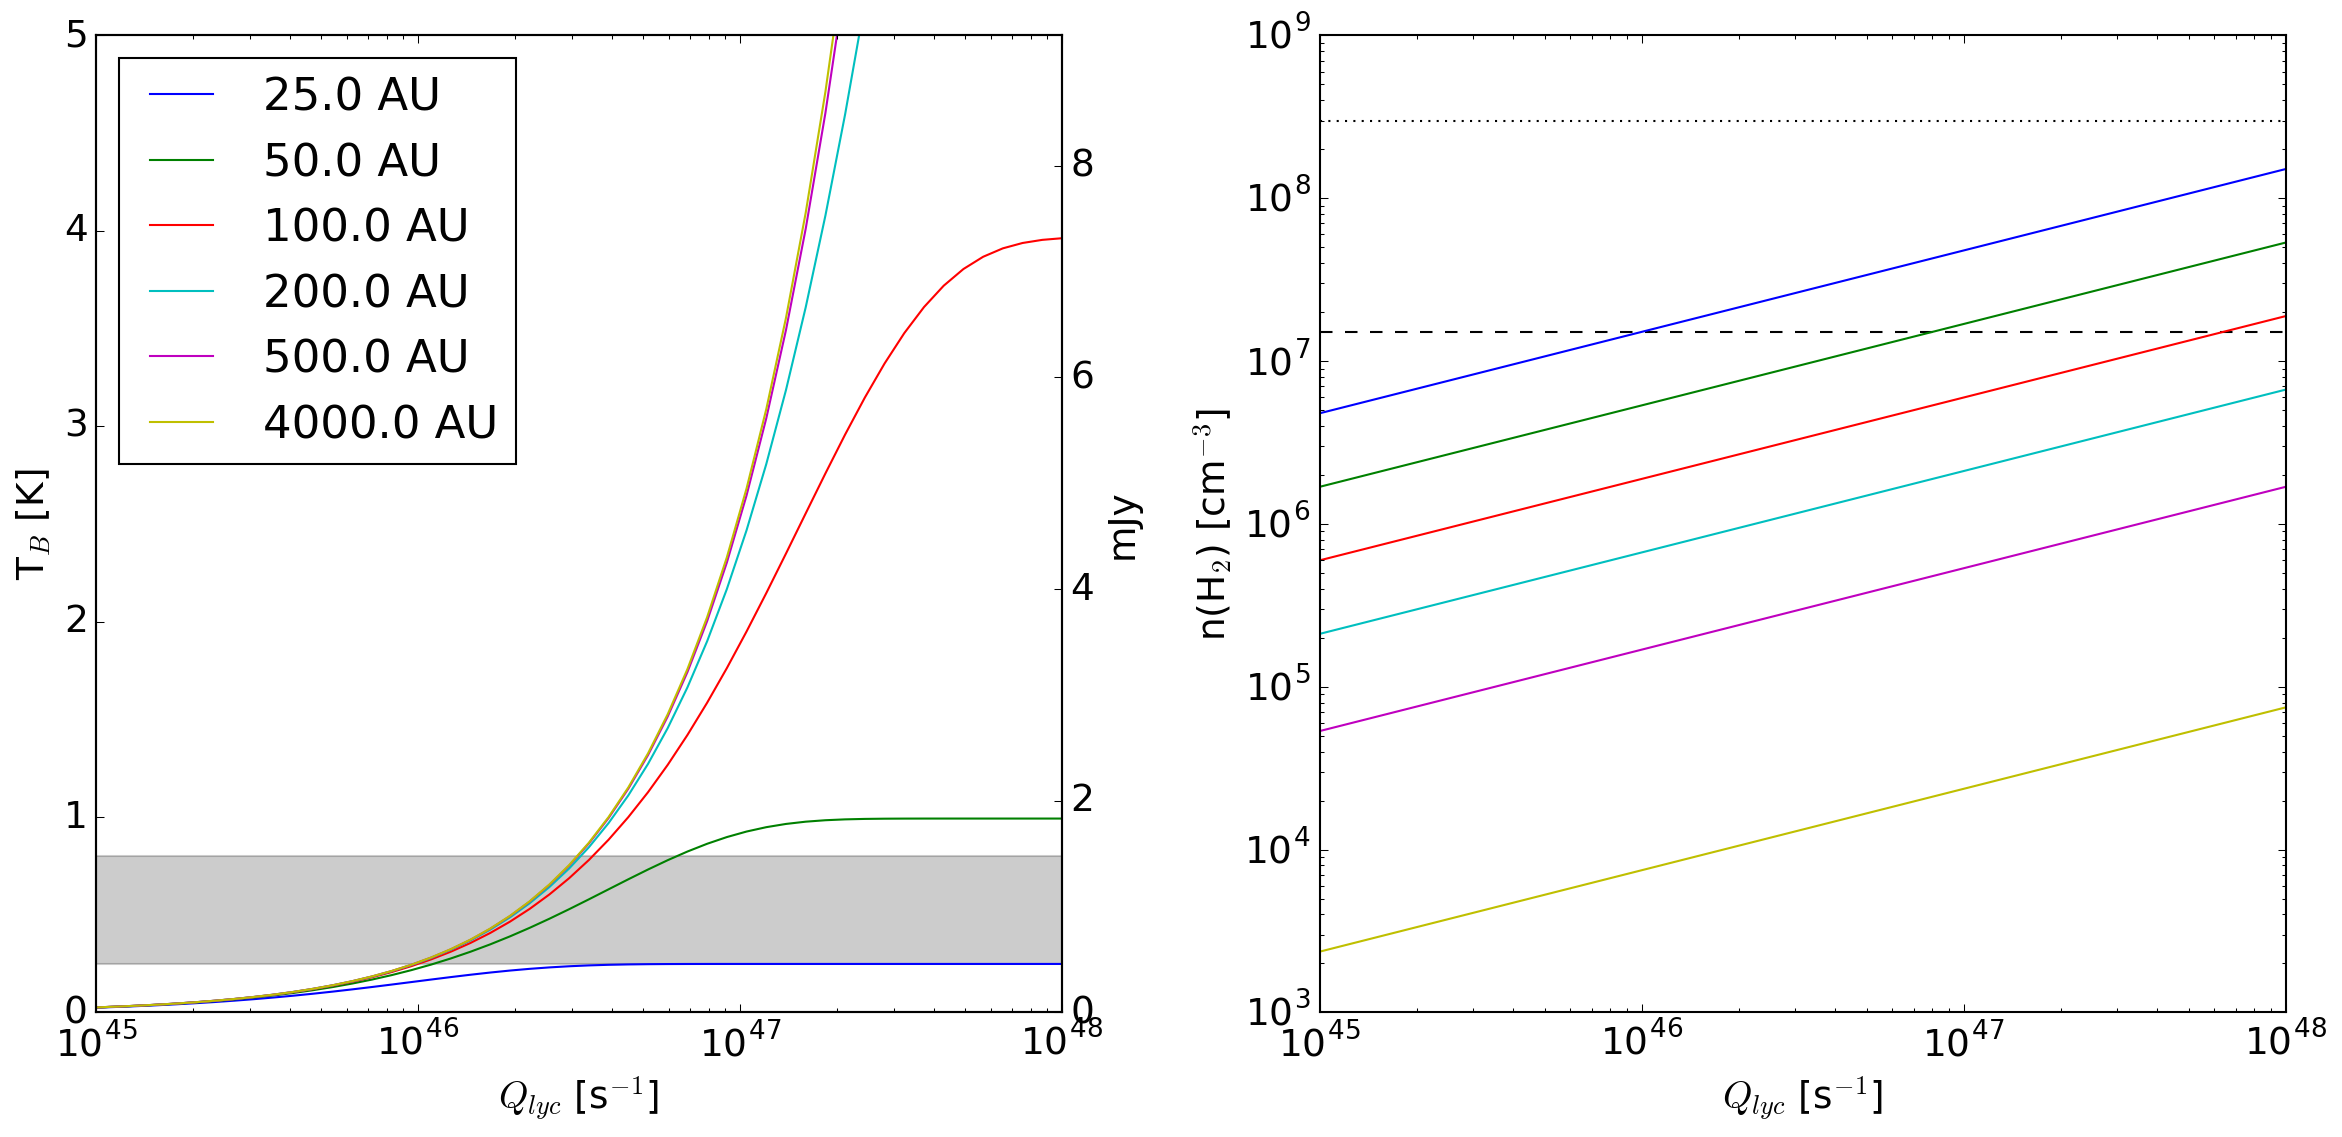
\includegraphics[scale=1,width=18cm]{figures/HII_region_brightness.png}
\caption{Simple models of spherical \hii regions to illustrate the observable
properties of such regions.  The \hii region size is shown by line color; the
legend in the left plot applies to both figures.  (left) The expected
brightness temperature (left axis) and corresponding flux density at 95 GHz
within a FWHM=0.5\arcsec beam (right axis) as a function of the Lyman continuum
luminosity for a variety of source radii.  The grey filled region shows the
range of our 5-sigma sensitivity limits,
which vary with location from 0.25 to 0.8 K.
(right) The density required to produce an \hii region of that radius.  The
horizontal dashed line shows the density corresponding to an unresolved dust
source ($r<0.2\arcsec=1700$ AU) at the 5-$\sigma$ detection limit ($\approx0.5$
mJy, or about 10 \msun of dust,
assuming $T=40$ K).    Above this line, dust emission would dominate over
free-free emission.  The dotted line shows the density required for dust
emission to produce a 10 mJy source at $T=40$ K.
The density has been scaled by a factor of two,
assumine $n_e = 2 n(\hh)$.
As seen in the left plot, for
any moderate-sized \hii region, $R>100$ AU, a high-luminosity star ($Q_{lyc} >
10^{47}$ \pers) would produce an \hii region brighter than the majority of our
sample, which includes only a few sources brighter than 10 mJy.  The electron
densities required to produce \hii regions within our observed range
($1<S_\nu<10$ mJy) are fairly extreme, $n_e\gtrsim10^6$ \percc, for O-stars.}
\label{fig:hiibrightness}
\end{figure*}



\subsubsection{Our hypothesis: The sources are (mostly) protostellar}
\label{sec:theyareprotostars}
After ruling out the other possibilities, we test and validate the hypothesis
that most or all of the sources are protostellar in this section.


\emph{General calculations:}
As noted at the top of this section, a cold `prestellar core' at our detection
limit would have $M(20\mathrm{K})\approx20$ \msun ($M(40\mathrm{K})\approx10$
\msun).  At these high densities ($n(20 \mathrm{K})\gtrapprox10^8$ \percc), it
is unlikely any such cores are unbound.  The high density required for our
sources results in a very short free-fall timescale, $t_{ff}\lessapprox6000$
yr, which suggests that the cores are unlikely to be prestellar cores and
instead, even if their emission is dominated by cold dust, they contain
protostars.  Their emission is likely dust-dominated, but is probably warmer
than the cloud average $T_D\sim20-40$ K.  

If we assume higher dust temperatures, the inferred gas mass is lower, but an
internal heating source - i.e., a protostar - is required.  For example,
if we assume $T_D=80$ K\footnote{At these dust temperatures,
we should be concerned about the assumed opacity, since ices
will begin to evaporate  \citep[e.g.,][]{Bergin1995a}, reducing the 3 mm
opacity and correspondingly increasing the required mass
required to produce the observed flux
\citep{Ossenkopf1994a}.  }, our detection limit is only $M(80\mathrm{K}) = 4
\msun$.  Heating that much dust well above the cloud average requires a
high-luminosity central heating source.

To constrain the required heating source, we examine the protostellar model
grid of \citet[][specifically, the \texttt{spubhmi} and \texttt{spubsmi}
models]{Robitaille2017a}.  The models that produce $S_{3 \mathrm{mm}} > 0.5$
mJy within a 5000 AU aperture uniformly have $L>10^4$ \lsun.  Such luminosities
imply either that an high-mass ($M\gtrsim8$ \msun) star has already formed and is still
surrounded by a massive envelope, or a high-mass YSO is present and accreting.
The models of \citet{Zhang2015f}, for example, generally only exhibit $L>10^4$
\lsun once a star has reached $M\approx10$ \msun as it continues to accrete to
a higher mass.  Similarly, pre-main-sequence stellar evolution models
\citep[e.g.,][]{Haemmerle2013a} only reach $L>10^4$ \lsun for stars with
final mass $M\gtrsim8$ \msun.  In the \citet{Robitaille2017a} model grid,
all sources with $L>10^5$ \lsun produce $S_{3 \textrm{mm}}>0.5$ mJy,
so our survey should be nearly complete to such sources, but in the range $10^4
\lsun < L < 10^5 \lsun$, a substantial fraction may be below our sensitivity
limit.





\emph{Comparison to similar data:}
We compare our detected sample to that of the Herschel Orion Protostar Survey
\citep[HOPS;][]{Furlan2016a} in order to get a general empirical sense of what
types of
sources we have detected.  We selected this survey for comparison because it is
one of the largest protostellar core samples with well-characterized bolometric
luminosities available.
Figure \ref{fig:hopshist} shows the HOPS source
flux densities at 870\um (from LABOCA on the APEX telescope) scaled to
$d=d_{Sgr B2}$ and 3 mm assuming a dust opacity index $\beta=1.5$,
which is shallower than usually inferred, so the extrapolated
fluxes may be slightly overestimated\footnote{\label{footnote:beta}
We err on the shallower side,
implying that the extrapolated 3 mm fluxes are brighter, since this approach
gives a more conservative view of the detectability of the Orion sources.
In reality, such sources are likely even fainter than predicted here.}.  The
870\um data
were acquired with a $\sim20\arcsec$ FWHM beam, which translates to a
resolution $\sim1\arcsec$ at $d_{Sgr B2} = $\dsgrb assuming $d_{Orion}=415$ pc,
so our beam size is somewhat smaller than theirs.

The HOPS sources are all fainter than the Sgr B2 sources.  The most luminous
and brightest HOPS source, with $L_{tot}<2000$ \lsun, would only be 0.2 mJy in
Sgr B2, or about a 2-$\sigma$ source - below our detection threshold even in
the noise-free regions of the map.  We  conclude that the Sgr B2 sources are
much more luminous than any in the Orion sample, which is consistent with all
of the sources in our sample being MYSOs.

% HOPS_core_plots

\begin{figure}[!htp]
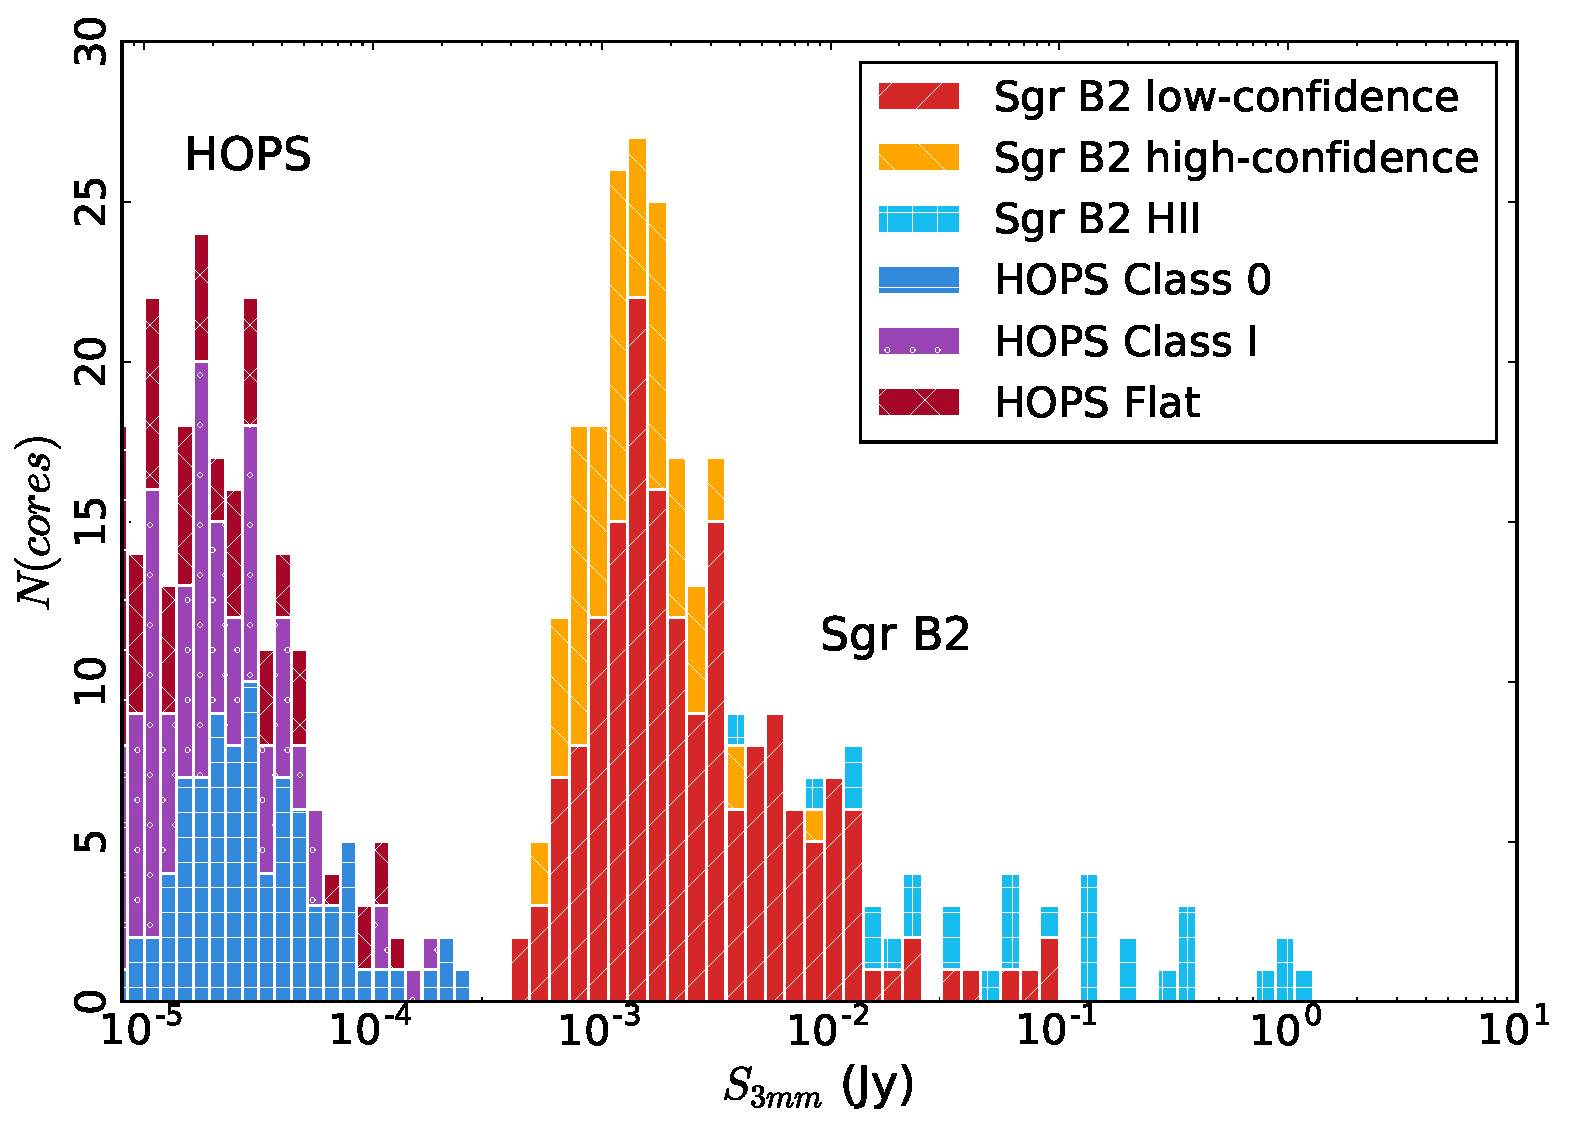
\includegraphics[scale=1,width=0.5\textwidth]{figures/core_peak_intensity_histogram_withHOPS.pdf}
\caption{A histogram combining the detected Sgr B2 cores with predicted flux densities
for sources at $d=\dsgrb$ and $\lambda=3$ mm
based on the HOPS \citep{Furlan2016a} survey.  The sources are labeled by their
infrared (2-20 \um) spectral index: Class 0 and I have positive spectral index
and flat spectrum sources have $-0.3 < \alpha_{IR} < 0.3$. The HOPS histogram
shows the 870 \um data from that survey scaled to 3 mm
assuming $\beta=1.5$ (see footnote \ref{footnote:beta}).
Every HOPS source is well below the detection threshold for our observations.}
\label{fig:hopshist}
\end{figure}


This conclusion is supported by a more direct comparison with the Orion nebula
as observed at 3 mm with MUSTANG \citep[][Figure
\ref{fig:orioncompare}]{Dicker2009a}.  Their data were taken at
9\arcsec FWHM resolution, corresponding to 0.48\arcsec at $d_{Sgr B2}$.  The
peak flux density measured in that map is toward Source I, $S_{90 GHz}(d_{Sgr
B2}) = 3.6$ mJy.  Source I\footnote{This source includes Source I, BN, and a few
other objects at this resolution, and at 3 mm Source I and BN are comparably
bright \citep{Plambeck2013a}.  This source is not part of the HOPS sample.}
would therefore  be detected and would be
somewhere in the middle of our sample.  It resides on a background of
extended emission, and the
extended component would be readily detected (and resolved) in our data. 
Source I is the only known high-mass YSO in the Orion cloud, and it would
be detectable in our survey while no other compact sources in the Orion cloud
would be.  This comparison supports the interpretation that most of the
non-\hii region sources are massive protostars.
%it appears
%safe to conclude that most of the detected sources that are not \hii regions
%are MYSOs.
%The M42 nebula would
%also be readily detectable, and is very similar in size and surface brightness
%to the \hii region Sgr B2 \hii T.

% Bontemps+ 2010: 3.5mm flux of N63 ~ 36 mJy, -> 1 mJy @ Sgr B2


\begin{figure}[!htp]
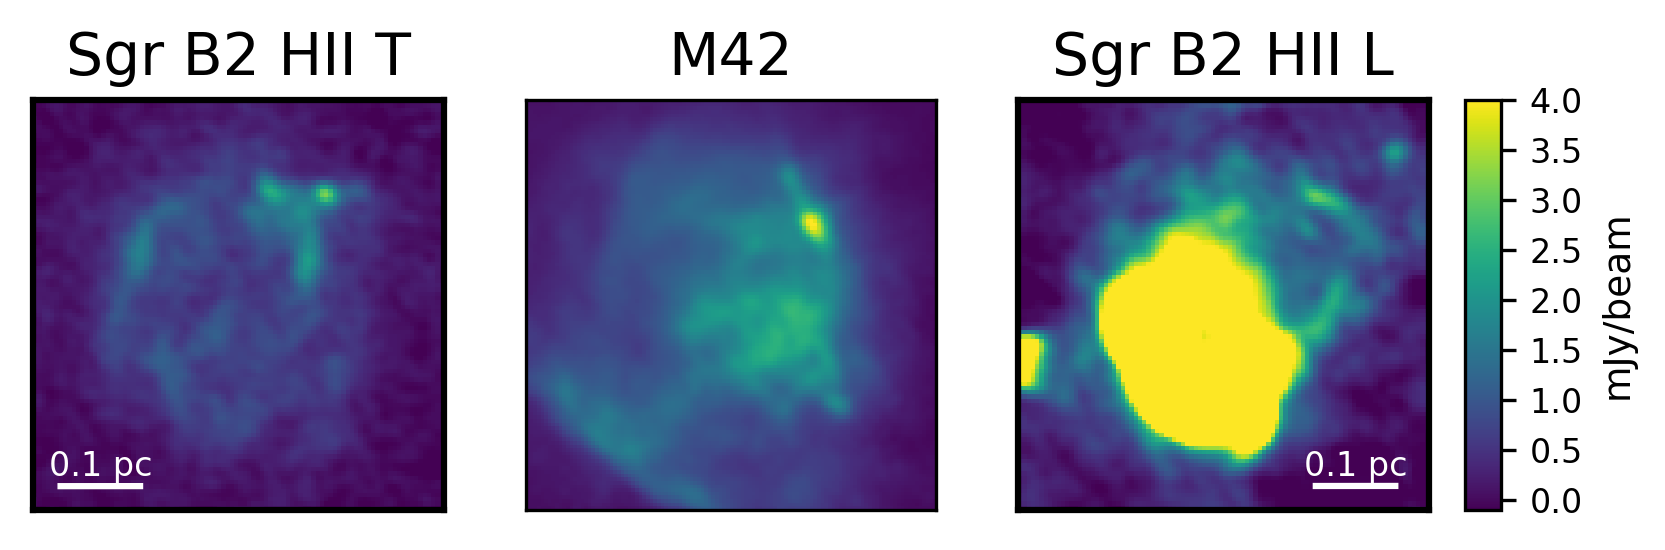
\includegraphics[scale=1,width=0.5\textwidth]{figures/Orion_SgrB2HII_side_by_side.png}
\caption{Comparison of two extended \hii regions in Sgr B2 (ALMA 3 mm continuum) to the
M42 \citep[GBT MUSTANG 3 mm continuum;][]{Dicker2009a} nebula in Orion.
The three panels are shown on the same physical and color scale assuming
$d_{Orion} = 415$ pc and $d_{Sgr B2} = $\dsgrb and that the ALMA and MUSTANG
data have the same continuum bandpass.  Sgr B2 \hii T is comparable in
brightness and extent to M42; Sgr B2 \hii L is much brighter and is saturated
on the displayed brightness scale.  The compact source to the top right of the
M42 image is Orion Source I; the images demonstrate that Source I and the entire
M42 nebula would be easily detected in our data.
}
\label{fig:orioncompare}
\end{figure}


While we have concluded that the sources are dusty, massive protostars, the
spectral indices we measured are somewhat surprising.  Typical dust clouds in
the Galactic disk have dust opacity indices $\beta\sim1.5-2$
\citep{Schnee2010a,Shirley2011a,Sadavoy2016a}.  Our spectral index measurements
are lower
than these, with only 3 sources (out of 62 with significant $\alpha$
measurements) having $\beta=\alpha-2 > 1.5$ (at the
$2\sigma$ level, up to 11 sources are consistent with $\beta=1.5$, but this is
primarily because of their high measurement error).  A shallower $\beta$
implies free-free contamination, large dust grains, or optically thick surfaces
are present within our sources.  Since the above arguments suggest that the
sources are high-mass protostars, the free-free contamination and optically
thick inner region models are both plausible.

\subsection{Source distribution functions and the star formation rate}
\label{sec:distributionsandsfr}

In this section we examine the distribution of observed flux densities and the
implied total stellar masses.  

% The flux density distribution of the non-\hii region sources follows a powerlaw
% with slope $\alpha=1.94\pm0.07$ \citep[fitted with the MLE method
% of][]{Clauset2007a}.  If we assume (incorrectly) that the stellar mass is linearly
% proportional to the 3 mm continuum flux density, this measurement implies a
% slope shallower than the $\alpha\sim2.35$ expected for a normal IMF.  It is
% possible that the IMF is genuinely different from Salpeter here, but it is more
% likely that the more massive stars are surrounded by warmer gas, implying that
% the source mass distribution is steeper than the source flux distribution.

If we make the very simplistic, but justified (Section
\ref{sec:theyareprotostars}), assumption that the sources we detect all contain
protostars with $L_{bol}\gtrsim10^4$ \lsun, and in turn make the related
assumption that each source either currently contains or will form into an
$M\gtrsim8 \msun$ star, we can infer the total (proto)stellar mass in the
observed region.

% Since we are assuming
% each star is at least a certain minimum mass, the values we derive here are
% most likely to be upper limits.  However, the additional caveat
% that our survey is not complete means that the estimates presented here are not
% strict limits in either direction, they are just approximate guesses.

We assume the
stellar masses based on the arguments in Section \ref{sec:theyareprotostars}:
in order to be detected, the sources must either be active OB stars
illuminating \hii regions, very compact cores with
$M>10$ \msun of warm dust within $R<4000$ AU, or
at least moderately-massive protostars within warm envelopes.  Note that the
mass estimates in this section are for the resulting stars, not their
envelopes.  The cluster affiliation for each source is reported in Table
\ref{tab:photometry}.

%Using a \citet{Kroupa2001a} mass function with $M_{max}=200$ \msun, 23\% of the
%mass is contained in $M>8\msun$ stars.  Using the lower-limit mass
%of $M=8\msun$ as the mass of each of our \ncores identified sources, we
%obtain a total mass $M(>8)=2100$ \msun.  The total stellar mass implied is
%$M_{tot} = 9\ee{3}$ \msun.  If instead we assume each source has a mass equal
%to the mean stellar mass over the IMF for $M>8$ \msun, $\bar{M}=21.1$ \msun,
%then the total inferred stellar mass is $M_{tot}=2.5\ee{4}$ \msun. 

%These are
%lower limits in the Sgr B2 N and M regions because our catalog is incomplete
%due to confusion and dynamic range limitations.  Additionally, we are using a
%single-star IMF and our resolution is only $\sim4000$ AU, so it is likely that
%we have undercounted by $\gtrsim2\times$, since high-mass stars have a high
%multiplicity fraction \citep{Mason2009a}.

% COMPARE TO SCHMIEDEKE

For each subcluster identified in \citet[][see Figure
\ref{fig:overview}]{Schmiedeke2016a}, we count the number of \hii regions
identified in our survey plus those identified in previous works
\citep{Gaume1995a,De-Pree1996a}, and we count the number of protostellar cores
not associated with \hii regions.  The distributions of source flux densities
associated with each cluster are shown in Figure \ref{fig:fluxhistclusters}.


\begin{figure}[!htp]
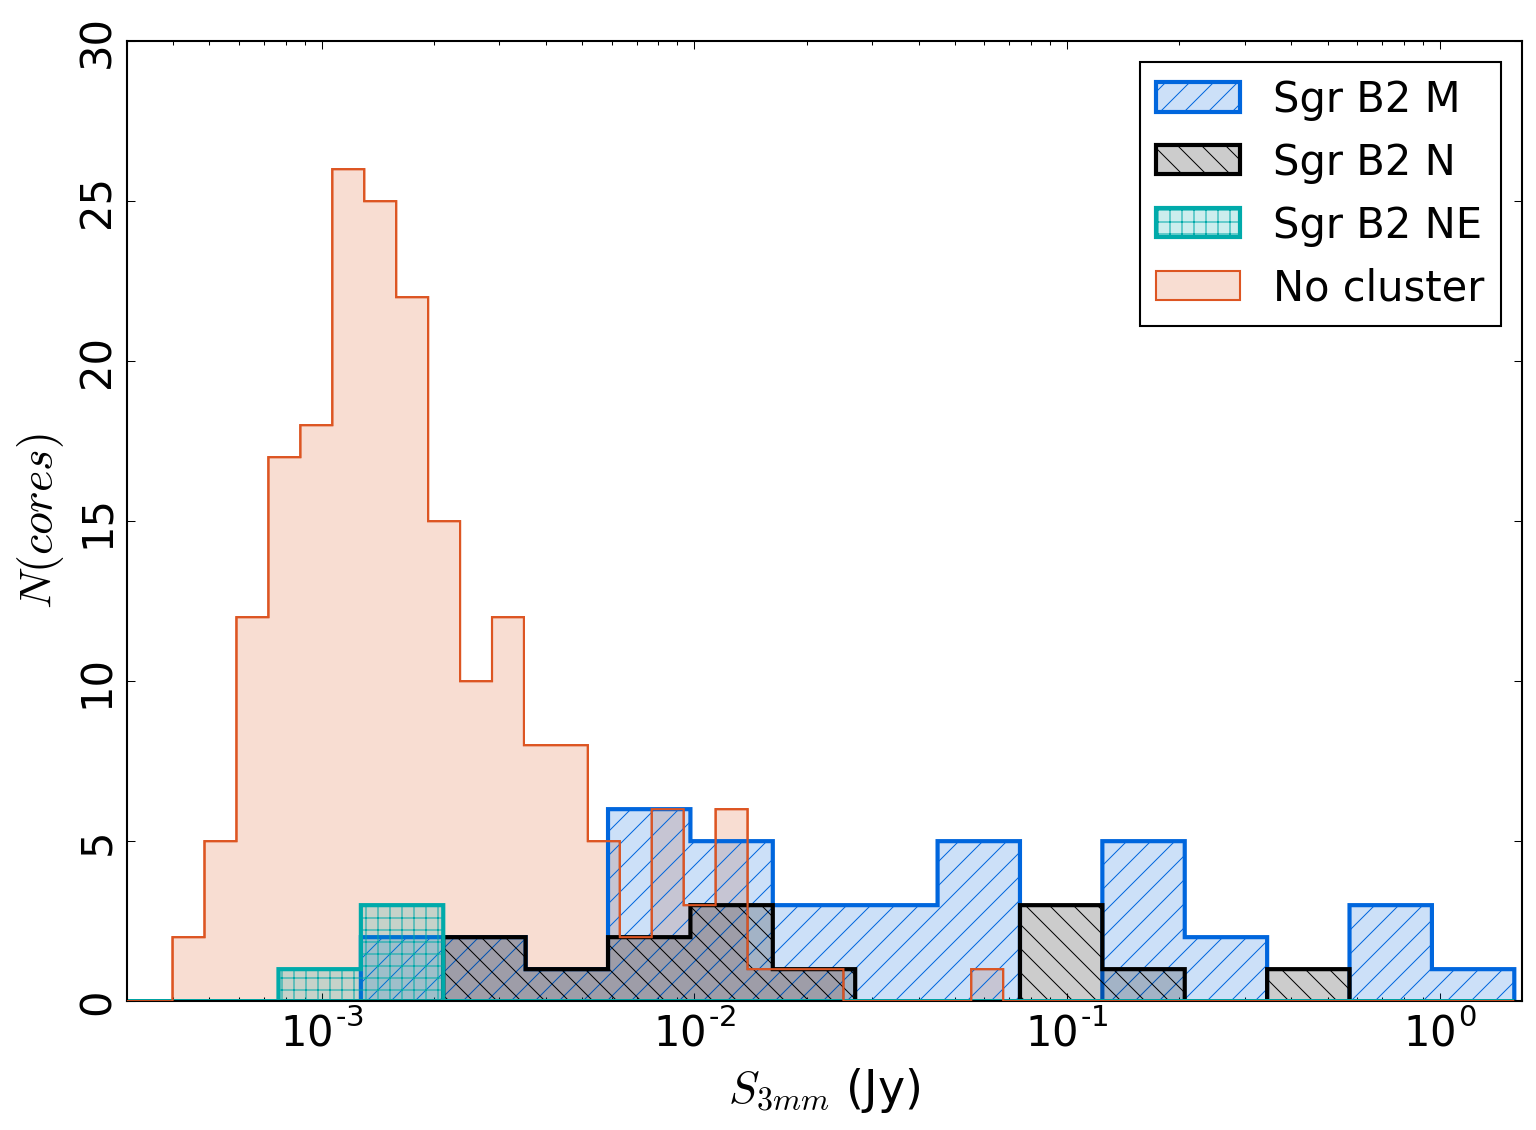
\includegraphics[scale=1,width=0.5\textwidth]{figures/core_peak_fluxdensity_coloredbycluster.png}
\caption{Histograms showing the flux density (the peak intensity converted to flux density
assuming the source is unresolved) of the observed sources classified by their
cluster association.  Unlike Figure \ref{fig:fluxhist}, the histograms are
overlapping, not stacked.  The bin widths for the clusters are wider than
for the unassociated sources.}
\label{fig:fluxhistclusters}
\end{figure}



We assume each source not associated with an \hii region contains or will form
a star with mass equal to
the average over the range 8-20 \msun assuming a \citet{Kroupa2001a} initial
mass function, $\bar{M}(8-20) = 12$ \msun (in this section, we refer
to these objects as ``cores'').  Based on the arguments in Section
\ref{sec:theyarehiiregions}, we assume each \hii region contains a star that is
B0 or earlier, and therefore that they each have a mass equal to the
average $\bar{M}(>20) = 45$ \msun.  In Table
\ref{tab:clustermassestimates}, the total counted mass estimate is shown as
$M_{count} = N \bar{M}$.

We also compute the \emph{total} stellar mass (i.e., the extrapolated mass
including low-mass stars) using the mass fractions $f(M>20)
= 0.14$ and $f(8<M<20)=0.09$.  The total mass is then $M_{inferred} =
M_{count}(M>20) / f(M>20) =
M_{count}(8<M<20) / f(8<M<20)$.  The inferred masses computed from \hii region
counts and from core counts are shown in columns $M_{inferred,\hii}$ and
$M_{inferred,cores}$ respectively. $M_{inferred}$ is the average of these two
estimates; it is also what would be obtained if all stars were assumed to be
average stars with $M>8$ \msun (and no upper limit).  If our mass range
classifications are
correct and the mass distribution is governed by a power-law IMF, we expect
$M_{inferred,\hii} = M_{inferred,cores}$.  In Sgr B2 N and S, the core-based
and \hii-region based estimates agree to
within a factor of 2, which is about as good as expected from Poisson noise in
the counting statistics.  

Sgr B2 M contains the largest source sample, and it has a factor of nine
discrepancy between the `core' and \HII-region based counts. The discrepancy
may arise from the combined effects of source
confusion at our 0.5\arcsec resolution and the increased noise around the
extremely bright central region that makes detection of $<2$ mJy sources
difficult.  The majority of pixels within the cluster region have significant
detections at 3 mm, but we do not presently have the capability to distinguish
between extended dust emission, free-free emission, or a confusion-limited
point source population.  While it is possible that this discrepancy
is driven by observational limitations, we also explore in Section
\ref{sec:clustersandextended} the possibility that it is a real physical
effect.

We compare our mass estimates to those of \citet{Schmiedeke2016a}, who inferred
stellar masses from \hii region counts.  The  two columns of Table
\ref{tab:clustermassestimates} with superscript $S$ show the observed and
estimated masses based on
\hii region counts.  For Sgr B2 M and N, our results are similar, as expected
since our catalogs are similar.  For S and NE, we differ by a large factor,
primarily because \citet{Schmiedeke2016a} assumed that $M_{min,YSO}$ and $M_{max}$
were the smallest and largest observed masses in the cluster, while we assumed
$M_{min,MYSO}=8$ \msun and $M_{max}=200$ \msun; i.e., we assumed a spatially
invariant IMF.

% cluster mass estimates table
% stellar_mass_estimates.py
\begin{table*}[htp]
\centering
\caption{Cluster Masses}
\begin{tabular}{cccccccccc}
\label{tab:clustermassestimates}
Name & $N(cores)$ & $N(H\textsc{ii})$ & $M_{count}$ & $M_{inferred}$ & $M_{inferred, H\textsc{ii}}$ & $M_{inferred, cores}$ & $M_{count}^s$ & $M_{inf}^s$ & SFR \\
 &  &  & $\mathrm{M_{\odot}}$ & $\mathrm{M_{\odot}}$ & $\mathrm{M_{\odot}}$ & $\mathrm{M_{\odot}}$ & $\mathrm{M_{\odot}}$ & $\mathrm{M_{\odot}}$ & $\mathrm{M_{\odot}\,yr^{-1}}$ \\
\hline
M & 17 & 47 & 2300 & 8800 & 15000 & 2300 & 1295 & 20700 & 0.012 \\
N & 11 & 3 & 270 & 1200 & 980 & 1500 & 150 & 2400 & 0.0017 \\
NE & 4 & 0 & 48 & 270 & 0 & 540 & 52 & 1200 & 0.00037 \\
S & 5 & 1 & 110 & 500 & 330 & 680 & 50 & 1100 & 0.00068 \\
Total & 240 & 57 & 5500 & 26000 & 19000 & 33000 & 1993 & 33400 & 0.035 \\
\hline
\end{tabular}
\par
$M_{count}$ is the mass of directly counted protostars, assuming each millimeter source is 12.0 \msun, or 45.5 \msun if it is also an \hii region.  $M_{inferred,cores}$ and $M_{inferred,\hii}$ are the inferred total stellar masses assuming the counted objects represent fractions of the total mass 0.09 (cores) and 0.14 (\hii regions).  $M_{inferred}$ is the average of these two.  $M_{count}^s$ and $M_{inf}^s$ are the counted and inferred masses reported in \citet{Schmiedeke2016a}.  The star formation rate is computed using $M_{inferred}$ and an age $t=0.74$ Myr, which is the time of the last pericenter passage in the \citet{Kruijssen2015a} model.  The \emph{total} column represents the total over the whole observed region.    The clusters sum to much less than the \emph{total} because the Deep South region is not included, and it dominates the overall core count.
\end{table*}
 
Finally, we estimate the star formation rate using the above mass estimates.
To determine the star formation rate, we need to know the age of the current
star forming burst.  We use the dynamical model of \citet{Kruijssen2015a} to
get an age of the Sgr B2 cloud $t=0.74$ Myr \citep{Longmore2013a}.  We divide
the inferred stellar mass by this age; the results
are shown in Table \ref{tab:clustermassestimates}.  This rate assumes that star
formation was initiated at the cloud's most recent pericenter passage.  Our
estimated total inferred SFR of the Sgr B2 cloud is 0.038 \msun \peryr, between
one quarter and one half of the total for the CMZ
\citep{Longmore2013a,Barnes2017b}.  Because of the large number of assumptions
above, there is at least a factor-of-two uncertainty on this number.


% While we identified \ncores sources from the continuum data, since we have only
% a single continuum band available, it is difficult to classify most of these
% except to say that they are certainly forming or recently formed stars.
% However, for a small subset, we have spectral line detections in either
% molecular or ionized species that tell us qualitatively whether a source is
% ionizing an \hii region or is surrounded by interesting molecular species.
% 
% \todo{Continue here - give the subset of sources with good line IDs (which is
% probably a by-hand process) and show example spectra of something not Sgr B2 M
% or N}

\subsection{An examination of star formation thresholds}
\label{sec:thresholds}
Several authors \citep[e.g.,][]{Lada2010a,Heiderman2010a} have proposed that star
formation can only occur above a certain density or column density
threshold\footnote{Column density is commonly used as a proxy for volume
density because of its observational convenience, but volume density is the
more meaningful physical parameter for most relevant processes in star formation
(e.g., gravity and pressure).}.  \citet{Kruijssen2014c} suggested that the
column density threshold in the CMZ should be higher than that in local clouds
based on predictions from turbulence-based star formation theories
\citep{Krumholz2005c,Padoan2011b}.
We therefore discuss our measurements of column density thresholds in this
section.



\subsubsection{Comparison to Lada, Lombardi, and Alves 2010}
\label{sec:ladathreshold}
In this section, we compare the star formation threshold in Sgr B2 to that in
local clouds performed by \citet{Lada2010a}.  They determined that all star
formation in local clouds occurs above a column density threshold $M_{thresh} >
116$ \msun pc$^{-2}$, or $N_{thresh}(\hh) > 5.2\ee{21}$ \persc assuming the
mean particle mass is 2.8 amu \citep{Kauffmann2008a}.  We first note, then,
that \emph{all pixels} in our column density maps (Section \ref{sec:colmaps},
Battersby et al, in prep) are above this threshold by \emph{at least} a factor
of 10.

However, Sgr B2 is \dsgrb away from us in the direction of our Galaxy's
center, meaning there is a potentially enormous amount of material unassociated
with the Sgr B2 cloud along the line of sight.  This material may have column
densities as low as
5\ee{21} \persc or as high as 5\ee{22} \persc, as measured from relatively
blank regions in the Herschel column density map \citep[][and in
prep]{Battersby2011a}.  The
former value corresponds to
the background at high latitudes, $b\sim0.5$, while the latter  is
approximately the lowest seen within our field of view. 
%If the higher value is the 
%correct foreground, there must be a perfect vacuum surrounding the dense gas in
%the Sgr B2 cloud - the `hole' seen in Fig...TODO: show a hole figure.
Even with the very aggressive foreground value of 5\ee{22} \persc subtracted,
nearly the whole Sgr B2 cloud exists above the \citet{Lada2010a} threshold.
%We can therefore
%immediately rule out the possibility that there is a universal star formation
%column threshold, since a large fraction of the observed volume exhibits
%no hint at all of star formation activity.
%-What kind of stars are we sensitive to?  Are they?
%(this is now handled above)

To directly compare our observations to the star formation thresholds reported
in \citet{Lada2010a}, we examined the column density associated with each
millimeter continuum source.  The \citet{Lada2010a} data used a variable
resolution for the column density measurements toward their sample, ranging from
0.06-0.35 pc (equivalent to 1.5 to 9.2\arcsec at a distance of \dsgrb).  The
Herschel data we have available with per-pixel SED fits lack the resolution
needed to make a direct comparison to the Lada et al data set, but the SHARC
and SCUBA data have resolution approximately equivalent to that used in the
Orion molecular cloud in their survey (see Section \ref{sec:colmaps}).

Because the higher-resolution images only cover a narrow range of wavelengths
and cannot be used to directly measure the dust temperature, we adopt two
approaches to approximate the dust temperature.  First, we use a two fixed
temperatures bracketing the observed range in the Herschel maps ($\sim20-50$ K)
to produce column density maps from the SCUBA and SHARC data.  Second, we
interpolated the Herschel-derived temperature map on to the SHARC and SCUBA
grids and used the SHARC and SCUBA intensities with the interpolated
temperature to infer the higher-resolution column density.

Figure \ref{fig:corebackgroundcdf} shows the cumulative distribution function
of the column density associated with each identified continuum source; the
column density used is the nearest-neighbor pixel to the source in the column
density maps.  Even using the conservative maximum temperature $T_{dust}=50$ K
(resulting in the minimum column density), all of the sources exist at a column
density an order of magnitude higher than the Lada threshold, and they exist
above that threshold even if the foreground is assumed to be an extreme
$5\ee{22}$ \persc.  While all of the sources exist above this threshold, not
all pixels above this threshold contain protostars or protostellar cores; the
threshold is therefore a necessary, but not a sufficient, condition for
high-mass star formation.


The \citet{Lada2010a} sample used Spitzer observations of nearby clouds that
were nearly complete to stars at least as small as 0.5 \msun.  By contrast, as
discussed in Section \ref{sec:theyareprotostars}, our survey is sensitive only
to stars with $M\gtrsim8$ \msun.  The apparently higher column threshold either
means that there is a genuinely higher threshold for star formation in the CMZ
or that there is a higher threshold for high-mass star formation that may still
be universal.  

\subsubsection{Other Thresholds}
\label{sec:otherthresholds}

A theoretical threshold for high-mass star formation, $\Sigma > 1$ g \persc
($N(\hh) > 2\ee{23}$ \persc) was developed by \citet{Krumholz2008a}.   Nearly
all of the sources we have detected reside above this threshold (independent of
the assumed foreground contamination), and we determined our sources are all
likely to be massive protostars in Section \ref{sec:theyareprotostars}.
However, not all pixels with $\Sigma > 1$ g \persc are forming high-mass stars
(Figure \ref{fig:coldistributionwithoutstarformation}).  Again, we have
inferred the presence of a necessary but not sufficient star formation
threshold

However, there is another threshold in our data, $N(\hh)>1\ee{24}$ \persc,
above which the majority of the gas is associated with ongoing high-mass star
formation (Figure \ref{fig:coldistributionwithoutstarformation}).  This
threshold suggests that any gas reaching a column density $N(\hh)>10^{24}$
\persc over a $\approx0.5$ pc size scale (the resolution of our column density
maps) has more likely than not begun to form high-mass stars.  This column
density corresponds to a volume density $n(\hh)\approx10^5$ \percc assuming
spherical symmetry.


% non-column-density (i.e., cloud-based) thresholds cannot be examined here.
% {\color{red} Can this discussion be expanded by examining other thresholds?
% Diederik suggested Krumholz HMSF threshold, Kauffmann and Pillai threshold should
% be examined.}

% core_local_brightness

\begin{figure}[!htp]
\includegraphics[scale=1,width=0.5\textwidth]{figures/core_background_column_cdf.png}
\caption{
Cumulative
distribution functions of the background column density associated
with each identified 3 mm continuum source.  The column densities are computed
from a variety of maps with different resolution and assumed temperature.
The Herschel maps use SED-fitted temperatures (Battersby et al. in prep) at
25\arcsec resolution (excluding the 500 \um data point) and 36\arcsec resolution.
The SHARC 350 \um and SCUBA 450 \um maps both have higher resolution ($\sim10\arcsec$)
but no temperature information; we used an assumed $T_{dust}=20$ and $T_{dust}=50$ K
to illustrate the range of possible background column densities (hatched
red and blue).  The thick solid red and blue lines show the SHARC and SCUBA column
density images using Herschel temperatures interpolated onto their grids: these
curves are closer to the 20 K than the 50 K curve and serve as the best estimate
column density maps.  The SHARC data fail to go to a cumulative fraction of 1
because the central pixels around Sgr B2 M and N are saturated (the lower temperature
assumptions result in optical depths $>1$, which cannot be converted to column
densities using the optically thin assumption).  The vertical
dashed line shows the $N(\hh)=5.2\ee{21}$ \persc column density threshold from
\citet{Lada2010a}, and the vertical dotted line shows the the $N(\hh)=2\ee{23}$
\persc \citet{Krumholz2008a} threshold for high-mass star formation.}
\label{fig:corebackgroundcdf}
\end{figure}


% TODO: find someplace to include this figure?
% % plot_codes/pointsource_overlay_scuba_column.py
% \FigureOneCol{figures/cores_on_SCUBA_column_saturated.png}
% {Overlay of the core and \hchii region locations on the SCUBA column density map
% created by interpolating the Herschel-measured temperatures onto the SCUBA grid
% and assuming the dust is optically thin at 450 \um.  The square grid at the center
% shows a region affected by saturation in the Herschel data.
% Contours are shown at $N(\hh) = 2\ee{23}$ \persc (green dashed lines)
% and $N(\hh) = 5,10,50,100\ee{23}$ \persc (blue lines).
% As shown in Figure \ref{fig:corebackgroundcdf}, the threshold above which nearly
% all cores are found is high, but this figure shows that the core density is not
% well-correlated with the column density: there is a relative dearth of cores
% in the high-column north region and an overabundance in the moderate-column deep
% south region.
% }
% {fig:coresonscubacol}{1}{0.5\textwidth}

% \Figure{figures/flux_histograms_with_core_location_CDF.png}
% {Histograms of the brightness measured with a variety of instruments at
% different submillimeter bands with the cumulative distribution function (CDF)
% of the \emph{background} brightness surrounding each core superposed.  The
% X-axis units are arbitrary (because right now I don't know the units of all of
% these) except for column, which is in units of cm$^{-2}$ of \hh as derived from
% SED fits to Herschel data (Battersby+).  The grey line is of the observed
% region in Sgr B2 and the blue line is of G0.253+0.016.  The thick grey line is
% the CDF of core background brightness, and is labeled by the right axis.}
% {fig:fluxhist}{1}{\textwidth}

\subsubsection{Comparison to G0.253+0.016}
In G0.253+0.016 (The Brick, G0.253), very little star formation
has been observed
\citep{Longmore2013a,Johnston2014a,Rathborne2014a,Rathborne2015a} despite most
of the cloud existing above the locally measured \citet{Lada2010a} column
density threshold.  The column density distribution function for G0.253
is shown in Figure \ref{fig:bricksgrb2colcompare}.

The \citet{Rathborne2014a} and \citet{Rathborne2015a} ALMA 3 mm data are the
deepest observations of G0.253 in the millimeter regime to date, with a
sensitivity about $4\times$ better than ours, but a beam of 1.7\arcsec (similar
to that shown in Figure \ref{fig:overview}; compare to Figure 2 in both
Rathborne et al papers).  Despite the higher sensitivity of their data,
they detected only 3 compact continuum sources.  Similarly,
\citet{Kauffmann2013a} detected only one compact continuum source in their
(less sensitive) SMA.  By contrast, even in our coarse resolution data, which
have a worse sensitivity (RMS $\approx 0.25$ mJy beam$^{-1}$, $10\times$ worse
than Rathborne et al), dozens of compact sources are evident.  Our better
resolution was critical for identifying the hundreds of sources we have
identified, but it is nonetheless clear that the star formation activity is
much higher in Sgr B2 than G0.253.


Comparing Sgr B2 to G0.253, the majority of the Sgr B2 cloud is at higher
column than G0.253.  Star formation in Sgr B2 nearly all occurs
at a higher column than exists within G0.253 (Figure
\ref{fig:bricksgrb2colcompare}).  The dearth of observed cores in G0.253 is
therefore easily explained if there is a column density threshold for star
formation that is not reached in G0.253.  Given that the G0.253 observations
were deeper than our own, yet still identified almost no forming stars, it
appears more likely that there is a lack of star formation rather than simply a
lack of high-mass star formation.  Nonetheless, robust verification of this
hypothesis will require much deeper observations sensitive to low-mass stars
in both regions.

% core_local_brightness

\begin{figure}[!htp]
\includegraphics[scale=1,width=0.5\textwidth]{figures/compare_brick_sgrb2_colPDF.png}
\caption{Histograms of the column density of G0.253+0.016 (blue) and Sgr B2 (gray)
using the combined SCUBA 450 \um and Herschel 500 \um intensity with the
interpolated Herschel dust temperatures.  The cumulative distribution of core
`background' column densities in Sgr B2 is shown as a thick gray line, showing
that the densities at which stars are forming in Sgr B2 are barely
reached in G0.253.  The vertical dotted line is the \citet{Krumholz2008a}
threshold for high-mass star formation at $N(\hh)=2\ee{23}$ \persc, while
the \citet{Lada2010a} threshold is below the minimum value plotted here (see
Section \ref{sec:thresholds}).}
\label{fig:bricksgrb2colcompare}
\end{figure}


% \subsection{Cloud edge features - bubbles}
% The most prominent feature of our catalog is the spatial distribution of the
% sources.  The majority trace a long, linear feature aligned approximately
% north-south.  In this section, we identify the edges of clouds seen in
% \cyanoacetylene as candidate bubbles.  They will be discussed
% further in Section \ref{sec:expandingshells}.
% 
% We display a series of figures showing the peak intensity over a velocity range
% selected to highlight the bubble edges.  In each figure, an ellipse shows
% the approximate location of the bubble.  The bubbles are \emph{not} ellipses,
% but the ellipses generally encompass the relatively empty region within the
% purported bubbles.
% 
% \Figure{figures/channelmaps/hc3n_channelmap_bubble_DeepSouthBubble_max.png}
% {A peak intensity map of the \cyanoacetylene J=10-9 line over the velocity
% range 48 to 90 \kms with ...}

\section{Surface density relations: comparison to Gutermuth et al. 2011}
\label{sec:gutermuth}
Unlike \citet{Lada2010a}, who invoke a threshold followed by a linear star
formation law relating the gas to the stellar surface density,
\citet{Gutermuth2011a} concluded that star formation was best represented as
power-law relations between the stellar and gas mass surface densities.

We adopt the same approach used in \citet{Gutermuth2009a} and
\citet{Gutermuth2011a} to compare gas and stellar mass surface densities.  We
computed both the star-centric mass surface density using the 11th nearest
neighbor density and a gridded surface density.  We assume a mean mass per
source $\bar{M}(M>8~\msun)=21.8$ \msun, and that each such star represents 23\%
of the total stellar mass (see Section \ref{sec:distributionsandsfr}), i.e.,
each 3 mm source is treated as a ``cluster'' containing 95 \msun of stellar
mass\footnote{In previous
sections, we assigned different masses to different source classes, i.e., we
assigned higher masses to \hii regions than non-\hii regions.  For consistency
with \citet{Gutermuth2011a}, we assume a constant mass per source here, which
may result in a systematic underestimation of the stellar mass surface density
at the highest densities (since the \hii regions are preferentially
concentrated in clusters).}. The correlation is similar whether we use the
Herschel column density directly or the SCUBA or SHARC-based column density
maps (see Section \ref{sec:colmaps}).  

There are a few key differences between our data and those of
\citet{Gutermuth2011a}.  First, our \emph{minimum} detected column density is
$N(\hh)\approx10^{23}$ \persc, while in their sample, the \emph{maximum}
observed was $A_V=38$, or $N(\hh)=3.8\ee{22}$ \persc.  Even if we subtract
our upper-limit foreground estimate $N(\hh)=5\ee{22}$ from the entire
Sgr B2 map, nearly all of the detected sources reside in regions with column
densities well above the maximum reached in the local cloud sample.
Second, our 3 mm source sample is sensitive to only the youngest sources, either
the high-mass equivalent of Class 0/I sources (`hot cores' or HMYSOs), or
deeply embedded hypercompact \hii regions.  The Spitzer sample included both
Class I sources, with estimated ages $t\lesssim0.5$ Myr, and Class II sources, with
ages $0.5 < t < 5$ Myr.  Our sample is therefore biased young.  If the
age estimate for Sgr B2 from the dynamical models
\citep{Longmore2013a,Kruijssen2015a} is accurate, there should be about as many
Class II sources as Class I, given the standard ages, meaning our total mass
estimate may be as much as a factor of 2 underestimated.
Third, as noted above, we are sensitive to only high-mass sources, so we infer
a significant population that is not directly observed.

Despite the differences in method, the Sgr B2, Mon R2, and Ophiucus clouds have
similar instantaneous star formation efficiencies (SFE), $\epsilon =
M_*/(M_*+M_{gas})$.  Sgr B2 has $\epsilon=0.016$ or $0.018$ (without and with
the foreground subtracted), Mon R2 $\epsilon=0.019$, and Ophiucus $\epsilon
= 0.04$.  SFEs ranging from 0.01-0.08 are observed throughout Galactic center
clouds \citep{Barnes2017b}, so in terms of overall efficiency, these clouds
appear similar to local low-mass clouds.


% core_local_brightness.py
% surface_density_maps.py

\begin{figure*}[!htp]
\subfigure[]{ \includegraphics[scale=1,width=0.5\textwidth]{figures/stellar_vs_gas_column_density_gridNN11_herschel.pdf} }
\subfigure[]{ \includegraphics[scale=1,width=0.5\textwidth]{figures/stellar_vs_gas_column_density_starcentered_herschel.pdf} }
\caption{Plots of the protostellar mass surface density vs the gas mass surface density
as derived from Herschel SED fitting (Section \ref{sec:colmaps}).  The stellar
mass surface densities are computed using the 11th
nearest-neighbor distance assuming that each star represents
a mass of 95 \msun, extrapolated assuming a uniform IMF.  (a) shows the
densities computed on a 0.25 pc grid, with column density lower limits
indicated where the Herschel data are saturated,
while (b) shows
the protostar-centric surface densities; no lower limits are included in this
figure because interpolated mass surface densities are used instead.  The
shaded regions
show the extrapolations of the relations derived by \citet{Gutermuth2011a}
for Ophiucus (blue) and Mon R2 (green); their data cut off below a mass
surface density $\Sigma < 10^3$ \msun pc$^{-2}$. 
The blue dotted line shows the Ophiucus relation scaled down by
$50\times$ to overlap with our data.
The thick orange lines show realizations of the \citet{Gutermuth2011a} $\alpha=2$ star
formation relation at times 0.01, 0.1, and 0.74 Myr, from bottom to top.
Similarly, the thick red lines show realizations of the $\alpha=1$ star
formation relation at the same ages.
The arrows along
the bottom show the effect of subtracting a uniform foreground column
density of $N(\hh)=5\ee{22}$ \persc (1100 \msun pc$^{-2}$).
}
\label{fig:stellarvsmasscolumn}
\end{figure*}


Figure \ref{fig:stellarvsmasscolumn} shows the stellar mass surface density
$\Sigma_*$ plotted against the gas mass surface density $\Sigma_{gas}$.
Our data show a large scatter and are plausibly compatible with a
power-law index in the range 1-2, and therefore may be consistent with the
steep slopes ($\alpha\approx2$) \citet{Gutermuth2011a} derived.


Figure \ref{fig:stellarvsmasscolumn}  shows in orange three curves from the
\citet{Gutermuth2011a} $\alpha=2$ star formation relation, their Equation 7,
with $k=10^{-4}$ pc$^{2}$ \msun$^{-1}$ Myr$^{-1}$ and $\alpha=2$, at times
$t=0.01$, 0.1, and 0.74 Myr .  Only the youngest curve, with age 0.01 Myr,
overlaps with our data.  The three red curves, which are essentially lines in
this figure, show the $\alpha=1$ relation with $k=0.1$ Myr$^{-1}$ at the same
three ages, and it achieves reasonable agreement with our data for the $t=0.74$
Myr line ($k=0.1$ \permyr implies the 50\% depletion time $t_{sf}=7$ Myr).  The
$\alpha=2$ star formation relation  is only consistent with our
data for times earlier than $t<0.1$ Myr.  This inconsistency is due to the very
fast depletion time for this form of star formation relation, which decreases
with gas surface density.  Indeed, the $\alpha=2$ star formation relation used
by \citet{Gutermuth2011a} is completely implausible for the gas surface density
regime we observe, as it implies that gas with an initial surface density of
$\Sigma_{gas}=10^4$ \msun \perspc would achieve a star formation efficiency
$\epsilon>1$ in $t<0.1$ Myr.  Our data are clearly incompatible with the
$\alpha=2$ relation but are reasonably compatible with a linear $\alpha=1$
relation with the same normalization used by \citet{Gutermuth2011a}.
%The relation we observe (Figure \ref{fig:stellarvsmasscolumn}) is several
%orders of magnitude lower than that extrapolated from \citet{Gutermuth2011a}.


%{\color{red} todo: move or summarize this in discussion/conclusion/abstract?}
%Our data are consistent with the slopes, but not the amplitude, of the
%\citet{Gutermuth2011a} results. 
Figure \ref{fig:stellarvsmasscolumn} also shows that the extrapolated relation
from the low-mass clouds exceeds our observations by at least $50\times$
(Ophiucus) or closer to $10^3\times$ (Mon R2).   The discrepancy between our
observations and theirs indicates either that there is a systematic tendency to
overestimate $\Sigma_*$ at high $\Sigma_{gas}$ in the Spitzer observations,
which seems unlikely, or that there is a different star formation relation in
Sgr B2 than in local clouds.


While a linear relation $\Sigma_* \propto \Sigma_{gas}$ can approximately
account for both local clouds and Sgr B2 as a whole, we have not yet explained
why the extrapolation of the observed $\Sigma_* - \Sigma_{gas}$ relation from
local clouds does not match Sgr B2.  We evaluate several possibilities here:

\begin{itemize}
    \item \emph{Could we be missing an older generation?}
        \citet{Gutermuth2011a} were sensitive to, and included in their sample,
        an older generation of Class II sources, which we cannot detect.
        However, they typically found a Class II / Class I ratio of only
        $\approx4\times$ \citep{Gutermuth2009a} (and they found that this
        ratio \emph{decreased} at higher gas surface densities), so the
        discrepancy cannot be exclusively due to our insensitivity to older
        YSOs unless the star formation rate within Sgr B2 was an order of
        magnitude higher 1-5 Myr ago.  Such an enhanced SFR is implausible
        since such a large population of massive stars would still be alive and
        very easily detectable in our survey and previous VLA surveys. 

    \item \emph{Could we be overestimating the gas mass?}
        The surface densities we measure cannot be substantially incorrect.
        Even if we assume the maximum plausible foreground cloud surface
        density of $N(\hh)=5\ee{22}$ \persc, the measured gas surface densities
        only shift by a small fraction (at most $50\%$, but typically $<10\%$
        for the star-centered measurements; see the arrows in Figure
        \ref{fig:stellarvsmasscolumn}).
        If the dust opacity or dust-to-gas ratio were substantially wrong,
        e.g., if the dust-to-gas ratio is 10 instead of 100, some of
        our data would begin to overlap with the local cloud data.
        If we have overestimated the gas mass by the required amount to
        bring out data into agreement with the local clouds, the star
        formation efficiency would be close to 50\% (i.e., $M_*\sim M_{gas}$),
        which is unlikely given the many signs of youth observed.

    \item \emph{Could there be high multiplicity in our sample?} 
        A possible explanation is that each of the detected sources in our
        sample is a high-number multiple system, such that each 3 mm source
        represents $\approx5000$ \msun instead of $\approx100$ \msun.  The
        multiplicity of the Orion Source I system suggests this interpretation
        is qualitatively plausible, but the factor of 50 required to match the
        \citet{Gutermuth2011a} extrapolation strains credibility.
        Additionally, the luminosity constraints from our observed data
        rule this possibility out unless the stellar IMF is bottom-heavy
        (see below for more IMF discussion).

    \item \emph{Could the sources be much more massive than we have inferred?}
        Another possibility is that each source we detect has a higher minimum
        mass than we have assumed, $M\gg8 \msun$, but again the required
        threshold is absurd, requiring each star to be $>100$ \msun to match
        the local cloud extrapolation.  Such massive stars are incompatible
        with the observed 3 mm luminosities for any plausible dust envelope
        or \hii region model (see Section \ref{sec:classification}).

    \item \emph{Could our sample be incomplete?}
        If our sample were incomplete by a factor of 100-1000, our results
        would match those extrapolated from Gutermuth et al.  While Section
        \ref{sec:contsources} concedes that the catalog may be incomplete, it
        is unlikely we are $<1\%$ complete, and the catalog is almost certainly
        complete to $>90\%$ for very massive and luminous sources ($L>10^5$
        \lsun, see Section \ref{sec:theyareprotostars}).  Additionally, if
        we were to include a factor of $100-1000\times$ more stellar mass, the 
        implied total stellar mass would be absurd, reaching $10^6-10^7$ \msun,
        exceeding the cloud mass.

    \item \emph{Could Sgr B2 consist of several Mon R2-like clouds stacked
        along the line of sight?}
        If there were $\sim50-100$ clouds of the same physical scale and
        surface density stacked along the line of sight, the data in Figure
        \ref{fig:stellarvsmasscolumn} would shift left, providing a possible
        explanation of the difference.  However, besides the extreme
        unlikeliness of having so many clouds along the line of sight, this
        explanation would require that the majority are non-star-forming, i.e.,
        they would have to be extremely young.  Also, the observations do not
        favor this scenario, as most of the star formation appears associated
        with a single velocity component in the \cyanoacetylene data (e.g., 
        Figure \ref{fig:coreson20cmandhc3n}, Appendix \ref{sec:hc3nfigures}).
        Finally, the elongation of the cloud on the sky hints that it is not
        multiple clouds, since they would have to all have similar elongations.

    \item \emph{Is the stellar IMF spatially nonuniform?}
        Our stellar mass surface density measurements are predicated on the
        assumption that each MYSO represents a fully-sampled initial mass
        function at the same location.  If there is any spatial non-uniformity
        in the IMF, e.g., if massive stars preferentially form at the bottoms
        of large potential wells (``primordial mass segregation''), the massive
        stars will have a different spatial distribution than the low-mass
        stars.  This effect would result in a higher measured stellar surface
        density at the highest gas surface densities and a lower measured
        stellar surface density at the lowest gas surface densities, i.e., it
        would result in a steeper slope in Figure
        \ref{fig:stellarvsmasscolumn}.  Therefore, unless there is inverse mass
        segregation, a spatially nonuniform IMF cannot explain our
        observations.

    \item \emph{Is the stellar IMF temporally nonuniform?}
        If high-mass stars form first, we would overestimate the stellar mass
        surface density.  However, if low-mass stars form first, we could
        underestimate the stellar mass surface density.  Given our survey's
        insensitivity to low-mass YSOs, the stellar mass surface density could
        be over an order of magnitude higher if it consists only of low-mass
        protostars.  Such a dramatic time sequencing effect in star formation
        would have profound implications for star formation studies, implying
        that any or all clouds currently forming low-mass stars may eventually
        form higher-mass stars, so testing this possibility with
        high-sensitivity observations should be a priority.

    \item \emph{Is the \emph{local} star formation efficiency lower at a fixed surface
        density in the Galactic center?}
        The overall star formation rate in the Galactic center is lower than
        expected given predictions from local clouds.  Changing the
        normalization of the star formation relation, i.e., reducing the prefactor
        $c=0.3$ to $c=0.01$, where $c$ is the fraction of gas in a core that
        makes it onto a star (the local efficiency), would allow our results to
        be consistent.  However, there is no evidence for any difference in the
        star formation process in the Galactic center once a core has formed;
        most evidence currently points to inefficient \emph{core} formation in
        the CMZ.

    \item \emph{Could the high star-formation threshold in the CMZ explain the
        difference?}
        As noted in Sections \ref{sec:ladathreshold} and
        \ref{sec:otherthresholds} above, forming stars only begin to appear
        above a threshold significantly higher than in local neighborhood
        clouds.  A simplistic model in which star formation simply does not
        occur below a fixed threshold does not explain the difference between
        our data and Gutermuth's, however, because the disagreement occurs at
        the high column densities in which we do observe star formation.
        However, a higher volume density threshold is plausible.  Such a threshold
        would imply a lower stellar density at fixed surface density, and would
        also permit variations in the stellar surface density based on how
        much dense gas is present.


%    \item \emph{Is the \emph{global} star formation efficiency lower at a fixed surface
%        density in the Galactic center?}
%        The linear relation that fits our data and (somewhat poorly) fits the
%        \citet{Gutermuth2011a} data has a constant $k=0.1$ \permyr, which
%        implies a star formation timescale, defined to be the time at which
%        half the initial gas is depleted by star formation,  $t_{sf} = 7$ Myr.

\end{itemize}

Of the items above, only the final, which suggests that a surface-density-based
star formation law is inviable, satisfactorily explains the discrepancy between
our data and the extrapolation from \citet{Gutermuth2011a}.

% In order to reconcile our measurements with
% theirs, either there must be a $\approx100\times$ larger population of more
% evolved stars (Class II equivalent, age 1-10 Myr) than young forming stars
% (Class 0/I equivalent), or the Sgr B2 cloud must be at a significantly earlier
% evolutionary stage than Mon R2 and the other clouds in their sample.
% A deep infrared observation in the high-extinction regions of the cloud,
% e.g., with JWST, would readily distinguish these possibilities.



\section{Discussion}
\label{sec:discussion}
We have reported the detection of a large number of point sources and inferred
that they are most likely all high-mass protostars.  These sources exclusively
reside in gas above $N(\hh)\gtrsim2\ee{23}$ \persc and are distributed along an
elongated  feature spanning the Sgr B2 cloud.

% \subsection{Thresholds}
% The column density threshold of $N(\hh)\gtrsim2\ee{23}$ \persc appears
% to be a necessary, but not sufficient, condition for high-mass star formation.  
% Above $N(\hh)>10^{24}$ \persc on scales of $\sim0.5$ pc, gas is more likely to
% have formed a high-mass star than not.
% 
% {\color{red}
% TODO: expand
% }

% In this section, we discuss
% the implications of this apparent threshold for high-mass star formation in the
% CMZ.



%While there is an apparent column density threshold required for high-mass
%stars to form, that threshold clearly forms only a necessary, not a sufficient,
%condition for star formation.  Figure
%\ref{fig:coldistributionwithoutstarformation} shows that there is abundant
%material within our observed region at $N>1$ g \persc that is not associated
%with ongoing high-mass star formation.  These high-column-density, low
%star-formation regions are also evident in Figure \ref{fig:coresonscubacol},
%which shows that the northern and western regions of the cloud are the
%deficient zones.

% nonstarforming_regions.py

\begin{figure}[!htp]
\includegraphics[scale=1,width=0.5\textwidth]{figures/column_density_distribution_with_and_without_SF.pdf}
\caption{Histograms of the column density measured with the combined SCUBA and Herschel
data using the interpolated Herschel temperatures covering only the region
observed with ALMA.  The black histogram shows the whole observed region,
the blue solid line shows the SCUBA pixels that do not contain an ALMA source,
and the red thick line shows those pixels that are within one beam
FWHM of an ALMA source.  While the ALMA sources (high mass protostars and young
stars)
clearly reside in high-column gas, there is abundant high-column material
that shows no signs of ongoing star formation.}
\label{fig:coldistributionwithoutstarformation}
\end{figure}


\subsection{What drives star formation in the greater Sgr B2 complex?}
\label{sec:whatdrives}
We have shown that, in addition to the known forming massive clusters,
star formation is ongoing in an extended and elongated region to the north
and south.  Why are the sources aligned?  Was star formation in Sgr B2
triggered by a single event?

There are a few different possible triggers that have been considered in the
literature: pericenter passage \citep[\S\ref{sec:pericenter};][]{Longmore2013a,Kruijssen2015a},
cloud-cloud collision
\citep[\S\ref{sec:ccc};][]{Hasegawa1994a,Mehringer1997a,Sato2000a}, and
expanding shells driven by
massive stars \citep[\S \ref{sec:expandingshells};][]{Martin-Pintado1999a}.
These scenarios are distinct and
apply to different scales.  The pericenter passage model assumes that gas is
fed into a $\sim100$ pc radius non-circular orbit and experiences significant
tidal compression at closest approach to the bottom of the gravitational
potential.  The compression leads to progressively increasing star formation
along the CMZ dust ridge.  Cloud-cloud collision models assume that independent
clouds on different orbits are interacting.  The expanding shell model assumes
the shells are driven by feedback from a previously formed generation of
high-mass stars.

We examine these three possibilities but reach no definitive conclusion about
which process is dominant.

\subsubsection{Pericenter Triggering}
\label{sec:pericenter}
Our observations are reconcilable with a star formation event triggered
at pericenter passage.  If the entire cloud was stable prior to pericenter
passage, at closest approach it would have been simultaneously crushed and
stretched by shear \citep{Kruijssen2015a}.  This event would have driven
collapse of the whole cloud, with the densest regions collapsing fastest and
possibly forming the clusters we observe today.  This model accounts for the
relative ages of the extended star formation event and the clustered starbursts
(discussed further in Section \ref{sec:clustersandextended}), but provides no
direct explanation for the morphology of the star formation event.

\subsubsection{Cloud-cloud collision}
\label{sec:ccc}
There are no definitive signs of `cloud-cloud collision' or `colliding flows'
in our line or continuum data, though that is largely because all possible
evidence for such flows is highly ambiguous. For example, \citet{Haworth2015c}
show some of the best cases for cloud-cloud collision using the `extended bridge'
in position-velocity between two colliding clouds, but these signatures can be 
completely hidden when multiple clouds exist along a line of sight or when
the clouds' intrinsic line widths are of the same magnitude as their impact velocity,
as in Sgr B2.  While multiple line components have been invoked as evidence
for cloud-cloud collision \citep{Hasegawa1994a,Corby2015a}, such multiple
components are also expected in turbulent cloud models.
We cannot strictly rule out cloud-cloud collision, but neither
can we provide evidence to support it; the kinematic features in our data are
compatible with multiple interpretations \citep[see also][who argued
that the multiple components cited as cloud-cloud collision evidence
could also be produced by opacity effects]{Henshaw2016a}.

Additionally, most of the notable kinematic features evident in the dense gas
images can be attributed to expanding \hii regions or otherwise feedback-driven
flows (see Section \ref{sec:expandingshells}).  While interacting independent
gas streams are a possible agent affecting Sgr B2, their effects are not
obvious in our core catalog or in the gas data cubes.

We note that some `colliding flows' are expected in almost any collapse
scenario.  For example, simulations of a cloud passing through Galactic
pericenter (Kruijssen et al. in prep.; Dale et al. in prep.) show that some
material is ejected during this passage that later collapses back onto the
original cloud.  It is possible that any apparent colliding flows
\citep[e.g.,][]{Sato2000a} are a component of this process.

\subsubsection{Expanding Shells}
\label{sec:expandingshells}
There is some evidence of expanding shells (bubbles) in Sgr B2
\citep{de-Vicente1997a,Martin-Pintado1999a}.  We compare the location of the
molecular gas traced by \cyanoacetylene and the location of the identified 3 mm
continuum sources to plausible bubble locations to evaluate whether the bubbles
may be responsible for driving the observed star formation.

% but these shells are not uniformly
% sites of star formation.
% There are four shell examples we consider: Sgr B2 DS, Sgr B2 N/NE,
% Sgr B2 E, and Sgr B2 W.  Two of these (N/NE and DS) show signs
% of star formation, two (E and W) do not.

There is extended ionized emission in Sgr B2 Deep South that appears to be a
bubble surrounded by the millimeter continuum sources.  While this region looks
like a normal \hii region in the 12\arcsec resolution 20 cm
VLA data in Figure \ref{fig:coreson20cmandhc3n}, the 3 mm continuum reveals long
filamentary features reminiscent of the Galactic center nonthermal filaments.  By
analogy, they may be magnetically dominated regions
\citep[e.g.,][]{LaRosa2004a}, but there must be some
central source of ionizing radiation or energetic particles.
\citet{Jones2011a} and \citet{Protheroe2008a} reported nonthermal
emission from this region, which they called Sgr B2 SC (``Southern Complex''),
supporting the idea that it is magnetically dominated. 
%They concluded that the nonthermal emission is not from secondary electrons
%from cosmic ray interactions, but did not provide an alternative hypothesis.
Whatever the
driver, it is possible that an expanding bubble of hot gas has compressed the
molecular material along the ridge where we observe star formation.
\citet{Martin-Pintado1999a} identified their bubbles B and F in this region,
and suggested that they are driven by Wolf-Rayet stellar winds, which is
consistent with both our continuum and line observations.  However, the ridge
of millimeter sources extends well above the apparent bubble edge, so it is
unlikely that the entire DS ridge was driven by a single coherent expanding
bubble.

By contrast, the Sgr B2 North bubble, which can be seen as arcs of
\cyanoacetylene emission in the top-left of Figure
\ref{fig:coreson20cmandhc3n}b, does not contain any ionized emission.  It
contains fewer total sources than DS, and these sources may trace the edge of
an expanding bubble previously noted by \citet{de-Vicente1997a}.  However,
unlike in DS, the sources are not well-correlated with the \cyanoacetylene
emission peaks, suggesting that the present bubble expansion is halting rather
than driving star formation in Sgr B2 N.

There are other regions within our map that have morphology suggestive of
expanding bubbles, but they cannot be definitively identified as bubbles.  In
Figure \ref{fig:coreson20cmandhc3n}b, there are several sharp-edged
\cyanoacetylene features, some of which are rounded and hint at the presence of
a central driving source. Figure \ref{fig:hc3nonscuba} shows that these ridges
are generally associated with high-column density dusty regions.  However, none
of these regions are associated with identified millimeter sources.  If they
are expanding shells, these shells are not driving star formation.

% Shell-like features in Sgr B2 E can be seen in Figure \ref{fig:hc3nonscuba}.
% The molecular gas, as traced by \cyanoacetylene in this case, outlines bubble edges to
% the east of Sgr B2 M: the \cyanoacetylene outlines a cavity in the column density map.
% The edge of this eastern bubble has a lower average column density than either
% the northern Sgr B2 NE or the Sgr B2 DS regions, and it shows no signs of
% ongoing star formation. 
% 
% In Sgr B2 W, there is a secondary ridge of \cyanoacetylene emission paralleling
% the central ridge.  No MYSOs are detected in this ridge.


%We observe that some sources appear to be associated with shells, but there are
%some shells that have no associated ongoing star formation.  Most of the
%observed star formation is not along shell edges.  We therefore conclude that,

While there may be expanding shells that have some effect on where MYSOs are
forming, it appears that in general, shells do not provide a sufficient
condition to drive star forming bursts.


% contour_overlays.py
%\FigureOneCol{figures/HC3N_contours_on_SCUBA_column.png}

\begin{figure*}[!htp]
\subfigure[]{ \includegraphics[scale=1,width=0.5\textwidth]{figures/HC3N_contours_on_SCUBA_column.png} }
\subfigure[]{ \includegraphics[scale=1,width=0.5\textwidth]{figures/HC3N_contours_on_SCUBA_column_withcores.png} }
\caption{ALMA \cyanoacetylene peak intensity contours (red) overlaid on the derived SCUBA
column density
image using Herschel Hi-Gal interpolated temperatures. The HC$_3$N was
shown in grayscale in Figure \ref{fig:coreson20cmandhc3n}.
Contours are at levels [3,7,11,15,19,23] K.  The  HC$_3$N bubble edges can be
seen surrounding cavities in the SCUBA column density map on the east side of
the main ridge.  To the north, the \cyanoacetylene also traces bubbles, but these are
less evident in this velocity-integrated view.  The important feature discussed
in Section \ref{sec:whatdrives} is the differing column density around each of
the bubbles.  The right figure has the cores overlaid as green dots,
showing that the 3 mm sources closely trace the molecular gas, but not all
dense molecular gas contains cores or protostars.}
\label{fig:hc3nonscuba}
\end{figure*}


\subsection{The clusters and the extended population}
\label{sec:clustersandextended}
We noted in Section \ref{sec:distributionsandsfr} that the \hii-region-inferred
protostellar mass matches the core-inferred protostellar mass to within a
factor of 2 in the whole Sgr B2 cloud and the individual clusters excepting Sgr
B2 M.  In Sgr B2 M, the \hii-region inferred mass is $\sim9\times$ greater than
the core-inferred mass.  While the lack of faint sources in Sgr B2 M could
be an observational limitation, it may be a real effect signifying an evolutionary
difference.

Sgr B2 M has more \hii regions and is more centrally condensed than any of the
other clusters and the distributed star forming population.  Assuming that \hii
regions represent a later stage in protostellar evolution than the dusty
protostellar core stage, the \hii region excess in Sgr B2 M implies that it is
older than Sgr B2 N and the distributed protostar population.  By contrast,
along the Sgr B2 DS ridge, there are no \hii regions, but there are $\sim100$
high-mass protostars, which implies that these protostars began their formation
nearly simultaneously.  Figure \ref{fig:fluxhistclusters} shows this difference
graphically; Sgr B2 M has an overall source flux distribution marginally higher
than Sgr B2 N but dramatically higher than the unclustered sources.

The large number of probable protostars observed along an elongated ridge
allows us to estimate an upper limit on their age.  Assuming all of these
forming stars are bound to the cloud and/or central clusters, they should
approach a spherical distribution within about one crossing time
\citep{Efremov1998a}.  If we assume the turbulent velocity dispersion is
$\sigma_{1D}\approx10$ \kms \citep[e.g.,][]{Henshaw2016a}, and the length of
the DS ridge is $L\approx10$ pc, the upper limit on the formation time of the
protostars is $L/\sigma_{1D}<1$ Myr.  Given the tight alignment of the
protostars with the gas ridge (Figures \ref{fig:coreson20cmandhc3n} and
\ref{fig:hc3nonscuba}), it is  possible to establish a stricter upper limit.  Most
of the sources are within $r<0.5$ pc of the `ridge', which, assuming they
formed in the ridge, suggests an upper age limit $t<r/\sigma_{1D}=5\ee{4}$ yr.
The DS ridge sources appear to be recently formed.

The expanding \hii regions observed around Sgr B2 M and N (and assumed to be
associated with them) give a lower limit on their ages \citep[assuming steady
expansion, which may not be a correct model][]{Peters2010b,De-Pree2014a}.  The
HII regions I, J, A1, and K4 have radii $r\approx0.1$ pc \citep{Gaume1995a},
suggesting their ages are at least $t>10^5$ yr assuming they are expanding into
a density $n\gtrsim10^5$ \percc \citep{De-Pree1995a,Schmiedeke2016a}.  The
clusters therefore appear to be somewhat older than the ridge sources.

% This argument doesn't work for me.
% If we assume the turbulent velocity dispersion is $\sigma_{1D}\approx10$ \kms
% \citep{Henshaw2016a}, and the crossing time is an upper limit on the age spread
% \citep[e.g.,][]{Efremov1998a}, we can infer the age spread in the clusters
% compared to that in the whole cloud.   The total size scale of the Sgr B2 cloud
% is $\sim10$ pc, which yields an ag spread upper limit $\lesssim 1$ Myr.  The
% clusters are much more compact, with $r<1$ pc, implying an age spread $<0.1$
% Myr.  

The relative ages of M and the rest of the region (i.e., Sgr B2 M is apparently
older) suggest two possibilities for their formation history.  If we take the
ages at face value, Sgr B2 M must have collapsed first to form stars in an
early event, then the DS ridge began forming stars in a
subsequent event.  A second possibility is that the overall collapse of both Sgr B2
M and DS began at the same time, but the Sgr B2 M region was denser and
therefore had a shorter collapse time, which is predicted by hierarchical
cluster formation models to lead to higher star formation efficiencies
\citep{Kruijssen2012a}.  Our catalog does not allow us to distinguish these
possibilities.  However, the latter scenario would predict that the cloud
should be in a state of global collapse, with the least dense regions
collapsing most slowly.  This collapse has been suggested to be ongoing in CMZ
clouds by \citet{Walker2015a,Walker2016a} and may leave detectable kinematic
signatures (e.g., self-absorption in moderately optically thick lines) in the
dense gas.


\citet{Yusef-Zadeh2009a} noted the presence of some Spitzer 4.5 \um excess
sources and 24 \um sources in the southern part of Sgr B2, and from these
detections concluded that star formation had proceeded outside-in in the Sgr B2
cloud.  Our data have revealed a much larger population of what are most likely
younger sources (dust-dominated protostars) in this region, which is
inconsistent with the previous interpretation.  Instead, it seems that the
central clusters are the oldest sites of star formation.  The excess of 4.5 \um
and 24 \um sources in DS may be because the cloud's envelope of opaque material
is thinner along those lines-of-sight.  We conclude that existing infrared
observations of the Sgr B2 cloud lack both the depth and resolution to detect
the significant ongoing star formation we report here.

\section{Conclusions}
\label{sec:conclusions}
We have reported the detection of \ncores 3 mm point sources in the extended
Sgr B2 cloud and determined that the majority are high-mass protostellar
cores.  This survey represents the first large population of protostars
detected in the Galactic center and represents the largest sample yet reported
of high-mass protostars.

The large population of high-mass protostellar cores indicates that an extended
region spanning the entire Sgr B2 cloud, not just the well-known clusters N, M,
and S, is undergoing a burst of star formation.  More than half of the
currently forming generation of stars is not associated with any of the
clusters but is instead part of the extended burst.

Using Herschel, SCUBA, and SHARC data, we have inferred a threshold for
high-mass star formation analogous to that inferred in local clouds by
\citet{Lada2010a}.  We find that there are no high-mass protostars in gas below
$N(\hh)<10^{23}$ \persc at a resolution of $\approx10\arcsec=0.4$ pc, and half
of the detected sources are found above $N(\hh)>10^{24}$ \persc.  However,
there is abundance material above $N(\hh)>10^{23}$ \persc that has no
associated protostars, indicating that this is a necessary, but not sufficient,
criterion for high-mass star formation.  These measurements imply either the
existence of a higher threshold for high-mass star formation than for low-mass,
as predicted by several theories, or a higher threshold for star formation in
the Galactic center as compared to local clouds \citep[e.g., as proposed
by][]{Kruijssen2014c,Rathborne2014a}.  Deeper observations, recovering the
low-mass sources, are required to distinguish these possibilities.

Comparing the protostellar mass surface density to the gas mass surface density
revealed a correlation compatible with the slopes observed by
\citet{Gutermuth2011a}, but with an amplitude significantly inconsistent with
theirs.  A star formation relation of the form $\Sigma_* \propto
\Sigma_{gas}^\alpha$ with $\alpha=2$ favored by \citet{Gutermuth2011a} cannot
explain our observations, though an $\alpha=1$ (linear) relation is consistent
with our data, and the $\alpha=1$ relation implies an age $t\sim1$ Myr that is
consistent with the \citet{Kruijssen2015a} dynamical model age for the Sgr B2
cloud $t=0.74$ Myr.

The extrapolation of the surface density relations from local clouds
in \citet{Gutermuth2011a} does not agree with our data.  We explored
a wide variety of possible explanations for the difference, and concluded
that the most likely is that a surface density relation is incapable
of explaining both local and CMZ clouds.  Instead, a volume-density
based model may be viable.


The large detected population of high-mass protostars implies a much larger
population of as-yet undetectable lower-mass protostars.  Future ALMA and JWST
programs to probe this population would provide the data needed to directly
compare star formation thresholds in the most intensely star-forming cloud in
our Galaxy to those in nearby clouds.

\software{
The software used to make this version of the paper is available from github at
\url{https://github.com/keflavich/SgrB2_ALMA_3mm_Mosaic/} with hash \githash
(\gitdate).  The tools used include \texttt{spectral-cube} and the \texttt{radio-astro-tools}
package (\url{https://github.com/radio-astro-tools/spectral-cube} and \url{radio-astro-tools.github.io}),
\texttt{astropy} \citep{Astropy-Collaboration2013a}, \texttt{astroquery}
(\url{astroquery.readthedocs.io}) and \texttt{CASA} \citep{McMullin2007a}.
}

\textit{Acknowledgements}
% reading these acknowledgements, you'd think this is the best-funded project
% ever...
The National Radio Astronomy Observatory is a facility of the National Science
Foundation operated under cooperative agreement by Associated Universities,
Inc.
This paper makes use of the following ALMA data: ADS/JAO.ALMA\#2013.1.00269.S.
ALMA is a partnership of ESO (representing its member states), NSF (USA) and
NINS (Japan), together with NRC (Canada), NSC and ASIAA (Taiwan), and KASI
(Republic of Korea), in cooperation with the Republic of Chile. The Joint ALMA
Observatory is operated by ESO, AUI/NRAO and NAOJ.
This work is partly supported by a grant from the National Science Foundation
(AST-1615311, De Pree).  JMDK gratefully acknowledges funding from the German
Research Foundation (DFG) in the form of an Emmy Noether Research Group (grant
number KR4801/1-1), from the European Research Council (ERC) under the European
Union's Horizon 2020 research and innovation programme via the ERC Starting
Grant MUSTANG (grant agreement number 714907), and from Sonderforschungsbereich
SFB 881 ``The Milky Way System'' (subproject P1) of the DFG.
RGM acknowledges support from UNAM-PAPIIT program IA102817.
JC acknowledges support for this work provided by the NSF through the Grote
Reber Fellowship Program administered by Associated Universities, Inc./National
Radio Astronomy Observatory.
ASM, PS and FM are partially supported by Deutsche Forschungsgemeinschaft
through grant SFB956 (subproject A6).



\bibliographystyle{aasjournal}
\bibliography{extracted} 
\appendix

\section{Single Dish Combination}
\label{sec:singledishcomb}
To measure the column density at a resolution similar to \citet{Lada2010a}, we
needed to use ground-based single-dish data with resolution $\sim10\arcsec$.
We combined these images with Herschel data, which recover all angular
scales, to fill in the missing `short spacings' from the ground-based data.

Specifically, we combine the SHARC 350 \um \citep{Dowell1999a} and 
SCUBA 450 \um \citep{Pierce-Price2000a,di-Francesco2008a} with Herschel 350 and
500 \um data \citep{Molinari2016a}, respectively.

Combining single-dish with `interferometer' data, or data that are otherwise
insensitive to large angular scales, is not a trivial process.  The standard
approach advocated by the ALMA project is to use the `feather' process, in
which two images are fourier-transformed, multiplied by a weighting function,
added together, and fourier transformed back to image space \citep[see
equations in \S 5.2 of][]{Stanimirovic2002a}.  This process is subject to
substantial uncertainties, particularly in the choice of the weighting
function.  

Two factors need to be specified for linear combination: the beam size of the
`single-dish', or total power, image, and the largest angular scale of the
`interferometer' or filtered image.  While the beam size is sometimes
well-known, for single dishes operating at the top of their usable frequency
range (e.g., the CSO at 350 \um or GBT at 3 mm), there are uncertainties in the
beam shape and area and there are often substantial sidelobes.  In
interferometric data, the largest angular scale is well-defined in the
originally sampled UV data, but is less well-defined in the final image because
different weighting factors change the recovered largest angular scale.  For
ground-based filtered data, the largest recoverable angular scale is difficult
to determine 
\citep[e.g.,][]{Ginsburg2013a,Chapin2013a}.

To assess the uncertainties in image combination, particularly on the
brightness distribution \citep[e.g.,][]{Ossenkopf-Okada2016a}, we have performed
a series of experiments combining the Herschel with the SCUBA data using
different weights applied to the SCUBA data.  As discussed in Section
\ref{sec:observations}, we empirically determined the scale factor required for
the best match between SCUBA and Herschel data was $3\times$, which is
 large but justifiable.  In the experiment shown in Figure
\ref{fig:feathercompare}, we show the images and resulting histograms when we
combine the Herschel data with the SCUBA data scaled by a range of factors from
$0.5\times$ to $10\times$.  The changes to the high end of the histogram are
dramatic, but the middle region containing most of the pixels (and most
relevant to the discussion of thresholds in the paper) is not substantially affected.
Additionally, we show the cumulative distribution function of core background
surface brightnesses (as in Figure \ref{fig:corebackgroundcdf}), showing again
that only the high end is affected. 


\begin{figure*}[!htp]
\includegraphics[scale=1,width=\textwidth]{figures/scuba_feather_scalefactor_comparison.pdf}
\caption{A demonstration of the effects of using different calibration factors when
combining the SCUBA data with the Herschel data using the `feather' process.
The numbers above each panel show the scale factor applied to the SCUBA data
before fourier-combining it with the Herschel data.  The factor of 3 was used
in this paper and shows the most reasonable balance between the high-resolution
of the SCUBA data and the all-positive Herschel data.  In the lower panels, the
fiducial scale factor of 3 is shown in black in all panels.  The solid lines
show histograms of the images displayed in the top panels.  The dashed lines
show the cumulative distribution of the background surface brightnesses of the
point sources in this sample; they are similar to the distributions shown in
Figure \ref{fig:corebackgroundcdf}.}
\label{fig:feathercompare}
\end{figure*}


\section{Self-calibration}
\label{sec:selfcal}
We demonstrate the impact of self-calibration in this section.  The adopted approach
used three iterations of phase-only self-calibration followed by two iterations of
phase and amplitude self-calibration.  Each iteration involved slightly
different imaging parameters.  The final, deepest clean used a threshold mask
on the previous shallower clean. The script used to produce the final images is
available at
\url{https://github.com/keflavich/SgrB2_ALMA_3mm_Mosaic/blob/\githash/script_merge/selfcal_continuum_merge_7m.py}.
The effects are shown with a cutout centered on the most affected region around
Sgr B2 M in Figure \ref{fig:selfcalprogression}.

% selfcal_progression

\begin{figure*}[!htp]
\includegraphics[scale=1,width=\textwidth]{figures/selfcal_progression_TCTE7m_try2_SgrB2M.pdf}
\caption{Progression of the self-calibration iterations.  The images show, from left to
right, the initial image, one, two, and three iterations of phase-only self
calibration, two iterations of phase and amplitude self-calibration,  a
reimaging of the 5th iteration with a deeper 0.1 mJy threshold using a mask at
the 2.5 mJy level, and finally, a sixth iteration of phase and amplitude
self-cal cleaned to 0.1 mJy over a region thresholded at 1.5 mJy.  All imaging
was done using two Taylor terms and multiscale clean.  The second row shows the
corresponding residual images.}
\label{fig:selfcalprogression}
\end{figure*}


\section{Photometric Catalog}
\label{sec:catalog}
We include the full catalog in digital form
(\url{https://github.com/keflavich/SgrB2_ALMA_3mm_Mosaic/blob/master/tables/continuum_photometry_withSIMBAD_andclusters.ipac}).
Table \ref{tab:photometry} shows
the brightest 35 sources; the rest are included in a digital-only catalog.
Sources are labeled based on an arbitrary source
number plus any pre-existing catalog name.  If a source is associated with a cluster,
it has an entry corresponding to that cluster in the \texttt{Cluster} column;
association is determined by checking whether a source is within a particular distance
of the cluster center as defined by \citet{Schmiedeke2016a}.  A source
\texttt{Classification} column is included, which states whether the source
is a strong or weak detection, whether it has an X-ray association, whether it
has a maser association, and its SIMBAD classification if it has one.
Measurements reported include the peak flux density $S_{\nu,max}$, the
corresponding brightness temperature $T_{B,max}$, the integrated flux density
within a beam (0.5\arcsec) radius, the background RMS flux level $\sigma_{bg}$
as an estimate of the local noise, the spectral index $\alpha$ and the error on
that $E(\alpha)$.  Mass and column density estimates are given for an assumed
temperature $T=40$ K ($M_{40K}$ and $N(\hh)_{40K}$).  For sources with
$T_{B,max}\gtrsim20$ K, these estimates are unlikely to be useful since the
assumed temperature is probably lower than the true temperature.
For sources with $T_{B,max}>40$ K, it is not possible to measure a mass
assuming $T=40$ K, so those entries are left empty.

\begin{table}[htp]
\caption{Continuum Source IDs and photometry}
\resizebox{\textwidth}{!}{
\begin{tabular}{llllllllllll}
\label{tab:photometry}
ID & Cluster & Classification & Coordinates & $S_{\nu,max}$ & $T_{B,max}$ & $S_{\nu,tot}$ & $\sigma_{bg}$ & $\alpha$ & $E(\alpha)$ & $M_{40K}$ & $N(\hh)_{40 K}$ \\
 &  &  &  & mJy bm$^{-1}$ & $\mathrm{K}$ & $\mathrm{mJy}$ & mJy bm$^{-1}$ &  &  & $\mathrm{M_{\odot}}$ & $\mathrm{cm^{-2}}$ \\
\hline
174 f3 & M & S\_\_W HII & 17:47:20.167 -28:23:04.809 & 1600 & 860 & 2400 & 46 & 0.89 & 0.002 & - & - \\
234 f4 & M & S\_\_W HII & 17:47:20.214 -28:23:04.379 & 1100 & 570 & 900 & 23 & 0.83 & 0.001 & - & - \\
176 f1 & M & S\_\_W HII & 17:47:20.127 -28:23:04.082 & 920 & 480 & 1400 & 30 & 1.2 & 0.006 & - & - \\
236 f10.303 & M & S\_\_W HII & 17:47:20.106 -28:23:03.729 & 890 & 460 & 800 & 19 & 1.1 & 0.015 & - & - \\
235 f2 & M & S\_\_W HII & 17:47:20.166 -28:23:03.714 & 820 & 430 & 670 & 33 & 1.3 & 0.002 & - & - \\
172 K2 & N & S\_\_W HII & 17:47:19.869 -28:22:18.466 & 370 & 200 & 650 & 49 & 2.5 & 0.018 & - & - \\
265 H & S & S\_\_W HII & 17:47:20.461 -28:23:45.404 & 360 & 190 & 580 & 3.9 & 0.65 & 0.019 & - & - \\
175 G & M & S\_\_W HII & 17:47:20.285 -28:23:03.162 & 340 & 180 & 390 & 5.6 & 0.68 & 0.03 & - & - \\
237 G10.44 & M & S\_\_W HII & 17:47:20.241 -28:23:03.387 & 280 & 140 & 160 & 15 & 0.69 & 0.006 & - & - \\
178 f10.37 & M & SX\_W HII & 17:47:20.178 -28:23:06 & 200 & 100 & 270 & 18 & 1.5 & 0.039 & - & - \\
171 K3 & N & S\_\_W HII & 17:47:19.895 -28:22:17.221 & 190 & 97 & 280 & 25 & 1.4 & 0.023 & - & - \\
177 B & M & S\_\_\_ HII & 17:47:19.918 -28:23:03.039 & 150 & 77 & 240 & 3.9 & 0.47 & 0.011 & - & - \\
241 f10.30 & M & S\_\_W HII & 17:47:20.106 -28:23:03.066 & 140 & 73 & 120 & 15 & 1.4 & 0.05 & - & - \\
179 f10.38 & M & S\_\_W HII & 17:47:20.193 -28:23:06.673 & 130 & 66 & 180 & 9.3 & 1.6 & 0.013 & - & - \\
180 E & M & S\_\_\_ HII & 17:47:20.108 -28:23:08.894 & 130 & 66 & 190 & 4 & 0.38 & 0.014 & - & - \\
173 K1 & N & S\_\_\_ HII & 17:47:19.78 -28:22:20.743 & 92 & 48 & 150 & 4.4 & 0.58 & 0.034 & - & - \\
170 & N & S\_\_W PartofCloud & 17:47:19.895 -28:22:13.621 & 92 & 48 & 160 & 23 & 1.7 & 0.082 & - & - \\
252 & N & S\_\_W denseCore & 17:47:19.862 -28:22:13.168 & 82 & 43 & 160 & 15 & 1.9 & 0.078 & - & - \\
225 f10.33b & M & SX\_W denseCore & 17:47:20.116 -28:23:06.374 & 69 & 36 & 100 & 14 & 1.9 & 0.21 & 1200 & 3.6\ee{26} \\
264 k4 & -- & S\_\_\_ HII & 17:47:19.997 -28:22:04.648 & 65 & 34 & 140 & 3.5 & 0.57 & 0.034 & 1100 & 2.6\ee{26} \\
96 Z10.24 & -- & S\_MW Maser & 17:47:20.039 -28:22:41.25 & 64 & 33 & 75 & 1.5 & 0.68 & 0.37 & 1100 & 2.5\ee{26} \\
181 D & M & S\_M\_ HII & 17:47:20.051 -28:23:12.91 & 59 & 31 & 94 & 1.3 & 0.64 & 0.088 & 990 & 2\ee{26} \\
240 f10.44b & M & S\_\_W HII & 17:47:20.252 -28:23:06.463 & 57 & 30 & 51 & 11 & 1.8 & 0.015 & 960 & 1.8\ee{26} \\
233 f10.27b & M & S\_\_W HII & 17:47:20.077 -28:23:05.383 & 50 & 26 & 78 & 18 & 2.3 & 0.18 & 840 & 1.4\ee{26} \\
239 & M & S\_\_W denseCore & 17:47:20.242 -28:23:07.222 & 45 & 24 & 46 & 8.6 & 2.3 & 0.091 & 760 & 1.1\ee{26} \\
244 C & M & S\_\_\_ - & 17:47:19.981 -28:23:18.437 & 35 & 19 & 67 & 0.49 & 0.47 & 0.081 & 600 & 7.8\ee{25} \\
242 f10.318 & M & S\_\_W HII & 17:47:20.129 -28:23:02.247 & 32 & 17 & 63 & 8.5 & 2.2 & 0.099 & 540 & 6.8\ee{25} \\
92 I10.52 & M & S\_\_\_ HII & 17:47:20.324 -28:23:08.2 & 32 & 17 & 45 & 5.3 & 0.63 & 0.061 & 530 & 6.6\ee{25} \\
245 A2 & -- & S\_\_\_ HII & 17:47:19.562 -28:22:55.916 & 25 & 13 & 32 & 2.1 & 0.54 & 0.025 & 410 & 4.8\ee{25} \\
109 & N & S\_\_W - & 17:47:19.901 -28:22:15.54 & 24 & 13 & 41 & 13 & 3.6 & 0.3 & 410 & 4.7\ee{25} \\
87 B9.99 & M & S\_\_\_ HII & 17:47:19.798 -28:23:06.942 & 23 & 12 & 37 & 1.9 & 0.89 & 0.042 & 390 & 4.4\ee{25} \\
88 & M & S\_\_W - & 17:47:19.617 -28:23:08.26 & 23 & 12 & 34 & 2.9 & 3.1 & 0.18 & 380 & 4.3\ee{25} \\
151 B10.06 & M & S\_M\_ HII & 17:47:19.86 -28:23:01.5 & 21 & 11 & 31 & 1.3 & 0.19 & 0.79 & 350 & 3.8\ee{25} \\
98 & -- & S\_M\_ Maser & 17:47:19.53 -28:22:32.55 & 18 & 9.5 & 29 & 0.36 & 3.2 & 1.1 & 300 & 3.3\ee{25} \\
\hline
\end{tabular}
}\par
The Classification column consists of three letter codes as described in Section \ref{sec:classification}.  In column 1, \texttt{S} indicates a strong source, \texttt{W} indicates weak or low-confidence source. In column 2, an \texttt{X} indicates a match with the \citet{Muno2009a} Chandra X-ray source catalog, while an underscore indicates there was no match.  In column 3, \texttt{M} indicates a match with the, \citet{Caswell2010a} Methanol Multibeam Survey \methanol maser catalog, while an underscore indicates there was no match.  Finally, we include the SIMBAD \citep{Wenger2000a} source object type classification if one was found.  The full electronic version of this table is available at \url{https://github.com/keflavich/SgrB2_ALMA_3mm_Mosaic/blob/master/tables/continuum_photometry_withSIMBAD_andclusters.ipac} and will be made available via the journal at the time of publication.
\end{table}
 
\section{Additional figures showing \cyanoacetylene}
\label{sec:hc3nfigures}
The \cyanoacetylene line was discussed at various points in the paper.  Because
the data are extremely rich and complex,  we include some additional figures
showing the detailed
structure of the lines here.


\begin{figure*}[!htp]
\includegraphics[scale=1,width=\textwidth]{figures/SgrB2_HC3N_channelmaps.pdf}
\caption{Channel maps of the \cyanoacetylene J=10-9 line.  Each panel shows the integrated
intensity over a 5 \kms velocity range as indicated on the figures.
The data shown here are 
12m+7m images made excluding the long-baseline data sets to emphasize
large angular scales
combined with total power
data by feathering the images.
The `ridge' feature  discussed in the text is most evident in the 50-55 \kms
channel, and these images show that it is dominated by a single velocity
component.
}
\label{fig:hc3nchannelmaps}
\end{figure*}



\begin{figure*}[!htp]
\subfigure[]{ \includegraphics[scale=1,width=0.5\textwidth]{figures/HC3N_peaktp.png} }
\subfigure[]{ \includegraphics[scale=1,width=0.5\textwidth]{figures/HC3N_peaktp05.png} }
\caption{Peak intensity maps of \cyanoacetylene J=10-9.
The left image shows the 12m short-baseline data combined with 7m and total
power data; by excluding the long-baseline data, the large angular scales are
emphasized.  The right image shows the robust 0.5-weighted 12m+7m data combined
with total power data;
it reaches a substantially higher peak intensity in the compact regions, but
the lower-intensity diffuse emission is relatively hidden.  In the right image,
the negative bowls seen near Sgr B2 M and N in this peak-intensity image
indicate that intermediate size scales were not well-recovered.  The bright
feature on the bottom-left of both images may be an imaging artifact.}
\label{fig:hc3npeakintensity}
\end{figure*}


\section{Additional figure showing Sgr B2 M and N}
\label{sec:onept3cm}
We show the Sgr B2 M and N source identifications overlaid on VLA 1.3 cm
continuum \citep{De-Pree2014a} in Figure \ref{fig:MandNzoomsVLA}.  This figure
highlights the differences between the wavelengths and provides a visual
verification that our classification of sources as \hii regions is reasonable.


\begin{figure*}[!htp]
\includegraphics[scale=1,width=\textwidth]{figures/cores_on_1.3cm_peak_MandN_zoomin_legend.pdf}
\caption{A close-up of Sgr B2 M and N similar to Figure \ref{fig:MandNzooms}, but with
VLA 1.3 cm continuum \citep{De-Pree2014a} in the background instead of the ALMA 3 mm
continuum.  Many of the features that appear in the 3 mm image do not appear
in the 1.3 cm image and are likely to be from dust emission, but the poorer sensitivity
of the 1.3 cm data also suggests that some of these features are simply 
free-free emission undeteted at 1.3 cm.}
\label{fig:MandNzoomsVLA}
\end{figure*}


\end{document}
